\documentclass[a4paper, 10pt]{report}

\usepackage[right=1in, left=1in, top=1in, bottom=1in]{geometry}
\linespread{1.5}
\usepackage{amsmath, amsthm, amssymb, amsfonts} %math's packages
\usepackage[utf8]{inputenc} %document encoding

\usepackage{enumerate}
\usepackage{verbatim}
%\usepackage{indentfirst}
\usepackage{graphicx}
\usepackage{algorithm}
\usepackage{algpseudocode}
\usepackage{listings}
\usepackage{color}
\usepackage{subcaption}
\usepackage{hyperref}
\usepackage{float}
\usepackage[T1]{fontenc}
\usepackage{makecell}
\usepackage{colortbl}
\usepackage{booktabs}
%\usepackage{babel}
\usepackage{array,multirow,graphicx}
\usepackage{pgfplots} %plots
\usepackage{standalone} %including other files without preambule
\usepackage{setspace}
\usepackage{tabu}
\usepackage{pdfpages}
\usepackage[round]{natbib}

\setlength{\parindent}{0pt}
\setlength{\parskip}{1ex}
% \setcounter{secnumdepth}{4}

% theorem
\theoremstyle{plain}
\newtheorem{theorem}{Theorem}[chapter]
\newtheorem{lemma}[theorem]{Lemma}
\newtheorem{proposition}[theorem]{Proposition}
\newtheorem{remark}[theorem]{Remark}
\newtheorem{corollary}[theorem]{Corollary}
\newtheorem{example}[theorem]{Example}


\renewcommand{\baselinestretch}{1.5}

%%%%% NEW MATH DEFINITIONS %%%%%

\usepackage{amsmath,amsfonts,amssymb,bm}

% independent sign
\newcommand{\indep}{\perp \!\!\! \perp}

% Mark sections of captions for referring to divisions of figures
\newcommand{\figleft}{{\em (Left)}}
\newcommand{\figcenter}{{\em (Center)}}
\newcommand{\figright}{{\em (Right)}}
\newcommand{\figtop}{{\em (Top)}}
\newcommand{\figbottom}{{\em (Bottom)}}
\newcommand{\captiona}{{\em (a)}}
\newcommand{\captionb}{{\em (b)}}
\newcommand{\captionc}{{\em (c)}}
\newcommand{\captiond}{{\em (d)}}

\newcommand{\iid}{\overset{\scriptstyle{\text{i.i.d.}}}{\sim}}

% Highlight a newly defined term
\newcommand{\newterm}[1]{{\bf #1}}


% Figure reference, lower-case.
\def\figref#1{figure~\ref{#1}}
% Figure reference, capital. For start of sentence
\def\Figref#1{Figure~\ref{#1}}
\def\twofigref#1#2{figures \ref{#1} and \ref{#2}}
\def\quadfigref#1#2#3#4{figures \ref{#1}, \ref{#2}, \ref{#3} and \ref{#4}}
% Section reference, lower-case.
\def\secref#1{section~\ref{#1}}
% Section reference, capital.
\def\Secref#1{Section~\ref{#1}}
% Reference to two sections.
\def\twosecrefs#1#2{sections \ref{#1} and \ref{#2}}
% Reference to three sections.
\def\secrefs#1#2#3{sections \ref{#1}, \ref{#2} and \ref{#3}}
% Reference to an equation, lower-case.
\def\eqref#1{equation~(\ref{#1})}
% Reference to an equation, upper case
\def\Eqref#1{Equation~(\ref{#1})}
% A raw reference to an equation---avoid using if possible
\def\plaineqref#1{\ref{#1}}
% Reference to a chapter, lower-case.
\def\chapref#1{chapter~\ref{#1}}
% Reference to an equation, upper case.
\def\Chapref#1{Chapter~\ref{#1}}
% Reference to a range of chapters
\def\rangechapref#1#2{chapters\ref{#1}--\ref{#2}}
% Reference to an algorithm, lower-case.
\def\algref#1{algorithm~\ref{#1}}
% Reference to an algorithm, upper case.
\def\Algref#1{Algorithm~\ref{#1}}
\def\twoalgref#1#2{algorithms \ref{#1} and \ref{#2}}
\def\Twoalgref#1#2{Algorithms \ref{#1} and \ref{#2}}
% Reference to a part, lower case
\def\partref#1{part~\ref{#1}}
% Reference to a part, upper case
\def\Partref#1{Part~\ref{#1}}
\def\twopartref#1#2{parts \ref{#1} and \ref{#2}}

\def\ceil#1{\lceil #1 \rceil}
\def\floor#1{\lfloor #1 \rfloor}
\def\1{\bm{1}}
\newcommand{\train}{\mathcal{D}}
\newcommand{\valid}{\mathcal{D_{\mathrm{valid}}}}
\newcommand{\test}{\mathcal{D_{\mathrm{test}}}}

\def\eps{{\epsilon}}

\newcommand{\ppx}[1]{\frac{\partial}{\partial #1}}
\newcommand{\pypx}[2]{\frac{\partial #1}{\partial #2}}
\newcommand{\ddx}[1]{\frac{d}{d #1}}
\newcommand{\dydx}[2]{\frac{d #1}{d #2}}

% Random variables
\def\reta{{\textnormal{$\eta$}}}
\def\ra{{\textnormal{a}}}
\def\rb{{\textnormal{b}}}
\def\rc{{\textnormal{c}}}
\def\rd{{\textnormal{d}}}
\def\re{{\textnormal{e}}}
\def\rf{{\textnormal{f}}}
\def\rg{{\textnormal{g}}}
\def\rh{{\textnormal{h}}}
\def\ri{{\textnormal{i}}}
\def\rj{{\textnormal{j}}}
\def\rk{{\textnormal{k}}}
\def\rl{{\textnormal{l}}}
% rm is already a command, just don't name any random variables m
\def\rn{{\textnormal{n}}}
\def\ro{{\textnormal{o}}}
\def\rp{{\textnormal{p}}}
\def\rq{{\textnormal{q}}}
\def\rr{{\textnormal{r}}}
\def\rs{{\textnormal{s}}}
\def\rt{{\textnormal{t}}}
\def\ru{{\textnormal{u}}}
\def\rv{{\textnormal{v}}}
\def\rw{{\textnormal{w}}}
\def\rx{{\textnormal{x}}}
\def\ry{{\textnormal{y}}}
\def\rz{{\textnormal{z}}}

% Random vectors
\def \rvalpha{{\bm{\alpha}}}
\def \rvbeta{{\bm{\beta}}}
\def\rvepsilon{{\mathbf{\epsilon}}}
\def\rvtheta{{\mathbf{\theta}}}
\def\rva{{\mathbf{a}}}
\def\rvb{{\mathbf{b}}}
\def\rvc{{\mathbf{c}}}
\def\rvd{{\mathbf{d}}}
\def\rve{{\mathbf{e}}}
\def\rvf{{\mathbf{f}}}
\def\rvg{{\mathbf{g}}}
\def\rvh{{\mathbf{h}}}
\def\rvu{{\mathbf{i}}}
\def\rvj{{\mathbf{j}}}
\def\rvk{{\mathbf{k}}}
\def\rvl{{\mathbf{l}}}
\def\rvm{{\mathbf{m}}}
\def\rvn{{\mathbf{n}}}
\def\rvo{{\mathbf{o}}}
\def\rvp{{\mathbf{p}}}
\def\rvq{{\mathbf{q}}}
\def\rvr{{\mathbf{r}}}
\def\rvs{{\mathbf{s}}}
\def\rvt{{\mathbf{t}}}
\def\rvu{{\mathbf{u}}}
\def\rvv{{\mathbf{v}}}
\def\rvw{{\mathbf{w}}}
\def\rvx{{\mathbf{x}}}
\def\rvy{{\mathbf{y}}}
\def\rvz{{\mathbf{z}}}
\def\rvE{{\mathbf{E}}}

% Elements of random vectors
\def\erva{{\textnormal{a}}}
\def\ervb{{\textnormal{b}}}
\def\ervc{{\textnormal{c}}}
\def\ervd{{\textnormal{d}}}
\def\erve{{\textnormal{e}}}
\def\ervf{{\textnormal{f}}}
\def\ervg{{\textnormal{g}}}
\def\ervh{{\textnormal{h}}}
\def\ervi{{\textnormal{i}}}
\def\ervj{{\textnormal{j}}}
\def\ervk{{\textnormal{k}}}
\def\ervl{{\textnormal{l}}}
\def\ervm{{\textnormal{m}}}
\def\ervn{{\textnormal{n}}}
\def\ervo{{\textnormal{o}}}
\def\ervp{{\textnormal{p}}}
\def\ervq{{\textnormal{q}}}
\def\ervr{{\textnormal{r}}}
\def\ervs{{\textnormal{s}}}
\def\ervt{{\textnormal{t}}}
\def\ervu{{\textnormal{u}}}
\def\ervv{{\textnormal{v}}}
\def\ervw{{\textnormal{w}}}
\def\ervx{{\textnormal{x}}}
\def\ervy{{\textnormal{y}}}
\def\ervz{{\textnormal{z}}}

% Random matrices
\def\rmA{{\mathbf{A}}}
\def\rmB{{\mathbf{B}}}
\def\rmC{{\mathbf{C}}}
\def\rmD{{\mathbf{D}}}
\def\rmE{{\mathbf{E}}}
\def\rmF{{\mathbf{F}}}
\def\rmG{{\mathbf{G}}}
\def\rmH{{\mathbf{H}}}
\def\rmI{{\mathbf{I}}}
\def\rmJ{{\mathbf{J}}}
\def\rmK{{\mathbf{K}}}
\def\rmL{{\mathbf{L}}}
\def\rmM{{\mathbf{M}}}
\def\rmN{{\mathbf{N}}}
\def\rmO{{\mathbf{O}}}
\def\rmP{{\mathbf{P}}}
\def\rmQ{{\mathbf{Q}}}
\def\rmR{{\mathbf{R}}}
\def\rmS{{\mathbf{S}}}
\def\rmT{{\mathbf{T}}}
\def\rmU{{\mathbf{U}}}
\def\rmV{{\mathbf{V}}}
\def\rmW{{\mathbf{W}}}
\def\rmX{{\mathbf{X}}}
\def\rmY{{\mathbf{Y}}}
\def\rmZ{{\mathbf{Z}}}

% Elements of random matrices
\def\ermA{{\textnormal{A}}}
\def\ermB{{\textnormal{B}}}
\def\ermC{{\textnormal{C}}}
\def\ermD{{\textnormal{D}}}
\def\ermE{{\textnormal{E}}}
\def\ermF{{\textnormal{F}}}
\def\ermG{{\textnormal{G}}}
\def\ermH{{\textnormal{H}}}
\def\ermI{{\textnormal{I}}}
\def\ermJ{{\textnormal{J}}}
\def\ermK{{\textnormal{K}}}
\def\ermL{{\textnormal{L}}}
\def\ermM{{\textnormal{M}}}
\def\ermN{{\textnormal{N}}}
\def\ermO{{\textnormal{O}}}
\def\ermP{{\textnormal{P}}}
\def\ermQ{{\textnormal{Q}}}
\def\ermR{{\textnormal{R}}}
\def\ermS{{\textnormal{S}}}
\def\ermT{{\textnormal{T}}}
\def\ermU{{\textnormal{U}}}
\def\ermV{{\textnormal{V}}}
\def\ermW{{\textnormal{W}}}
\def\ermX{{\textnormal{X}}}
\def\ermY{{\textnormal{Y}}}
\def\ermZ{{\textnormal{Z}}}

% Vectors
\def\vzero{{\bm{0}}}
\def\vone{{\bm{1}}}
\def\vmu{{\bm{\mu}}}
\def\vtheta{{\bm{\theta}}}
\def\va{{\bm{a}}}
\def\vb{{\bm{b}}}
\def\vc{{\bm{c}}}
\def\vd{{\bm{d}}}
\def\ve{{\bm{e}}}
\def\vf{{\bm{f}}}
\def\vg{{\bm{g}}}
\def\vh{{\bm{h}}}
\def\vi{{\bm{i}}}
\def\vj{{\bm{j}}}
\def\vk{{\bm{k}}}
\def\vl{{\bm{l}}}
\def\vm{{\bm{m}}}
\def\vn{{\bm{n}}}
\def\vo{{\bm{o}}}
\def\vp{{\bm{p}}}
\def\vq{{\bm{q}}}
\def\vr{{\bm{r}}}
\def\vs{{\bm{s}}}
\def\vt{{\bm{t}}}
\def\vu{{\bm{u}}}
\def\vv{{\bm{v}}}
\def\vw{{\bm{w}}}
\def\vx{{\bm{x}}}
\def\vy{{\bm{y}}}
\def\vz{{\bm{z}}}

% Elements of vectors
\def\evalpha{{\alpha}}
\def\evbeta{{\beta}}
\def\evepsilon{{\epsilon}}
\def\evlambda{{\lambda}}
\def\evomega{{\omega}}
\def\evmu{{\mu}}
\def\evpsi{{\psi}}
\def\evsigma{{\sigma}}
\def\evtheta{{\theta}}
\def\eva{{a}}
\def\evb{{b}}
\def\evc{{c}}
\def\evd{{d}}
\def\eve{{e}}
\def\evf{{f}}
\def\evg{{g}}
\def\evh{{h}}
\def\evi{{i}}
\def\evj{{j}}
\def\evk{{k}}
\def\evl{{l}}
\def\evm{{m}}
\def\evn{{n}}
\def\evo{{o}}
\def\evp{{p}}
\def\evq{{q}}
\def\evr{{r}}
\def\evs{{s}}
\def\evt{{t}}
\def\evu{{u}}
\def\evv{{v}}
\def\evw{{w}}
\def\evx{{x}}
\def\evy{{y}}
\def\evz{{z}}

% Matrix
\def\mA{{\bm{A}}}
\def\mB{{\bm{B}}}
\def\mC{{\bm{C}}}
\def\mD{{\bm{D}}}
\def\mE{{\bm{E}}}
\def\mF{{\bm{F}}}
\def\mG{{\bm{G}}}
\def\mH{{\bm{H}}}
\def\mI{{\bm{I}}}
\def\mJ{{\bm{J}}}
\def\mK{{\bm{K}}}
\def\mL{{\bm{L}}}
\def\mM{{\bm{M}}}
\def\mN{{\bm{N}}}
\def\mO{{\bm{O}}}
\def\mP{{\bm{P}}}
\def\mQ{{\bm{Q}}}
\def\mR{{\bm{R}}}
\def\mS{{\bm{S}}}
\def\mT{{\bm{T}}}
\def\mU{{\bm{U}}}
\def\mV{{\bm{V}}}
\def\mW{{\bm{W}}}
\def\mX{{\bm{X}}}
\def\mY{{\bm{Y}}}
\def\mZ{{\bm{Z}}}
\def\mBeta{{\bm{\beta}}}
\def\mPhi{{\bm{\Phi}}}
\def\mLambda{{\bm{\Lambda}}}
\def\mSigma{{\bm{\Sigma}}}

% Tensor
\DeclareMathAlphabet{\mathsfit}{\encodingdefault}{\sfdefault}{m}{sl}
\SetMathAlphabet{\mathsfit}{bold}{\encodingdefault}{\sfdefault}{bx}{n}
\newcommand{\tens}[1]{\bm{\mathsfit{#1}}}
\def\tA{{\tens{A}}}
\def\tB{{\tens{B}}}
\def\tC{{\tens{C}}}
\def\tD{{\tens{D}}}
\def\tE{{\tens{E}}}
\def\tF{{\tens{F}}}
\def\tG{{\tens{G}}}
\def\tH{{\tens{H}}}
\def\tI{{\tens{I}}}
\def\tJ{{\tens{J}}}
\def\tK{{\tens{K}}}
\def\tL{{\tens{L}}}
\def\tM{{\tens{M}}}
\def\tN{{\tens{N}}}
\def\tO{{\tens{O}}}
\def\tP{{\tens{P}}}
\def\tQ{{\tens{Q}}}
\def\tR{{\tens{R}}}
\def\tS{{\tens{S}}}
\def\tT{{\tens{T}}}
\def\tU{{\tens{U}}}
\def\tV{{\tens{V}}}
\def\tW{{\tens{W}}}
\def\tX{{\tens{X}}}
\def\tY{{\tens{Y}}}
\def\tZ{{\tens{Z}}}


% Graph
\def\gA{{\mathcal{A}}}
\def\gB{{\mathcal{B}}}
\def\gC{{\mathcal{C}}}
\def\gD{{\mathcal{D}}}
\def\gE{{\mathcal{E}}}
\def\gF{{\mathcal{F}}}
\def\gG{{\mathcal{G}}}
\def\gH{{\mathcal{H}}}
\def\gI{{\mathcal{I}}}
\def\gJ{{\mathcal{J}}}
\def\gK{{\mathcal{K}}}
\def\gL{{\mathcal{L}}}
\def\gM{{\mathcal{M}}}
\def\gN{{\mathcal{N}}}
\def\gO{{\mathcal{O}}}
\def\gP{{\mathcal{P}}}
\def\gQ{{\mathcal{Q}}}
\def\gR{{\mathcal{R}}}
\def\gS{{\mathcal{S}}}
\def\gT{{\mathcal{T}}}
\def\gU{{\mathcal{U}}}
\def\gV{{\mathcal{V}}}
\def\gW{{\mathcal{W}}}
\def\gX{{\mathcal{X}}}
\def\gY{{\mathcal{Y}}}
\def\gZ{{\mathcal{Z}}}

% Sets
\def\sA{{\mathbb{A}}}
\def\sB{{\mathbb{B}}}
\def\sC{{\mathbb{C}}}
\def\sD{{\mathbb{D}}}
% Don't use a set called E, because this would be the same as our symbol
% for expectation.
\def\sF{{\mathbb{F}}}
\def\sG{{\mathbb{G}}}
\def\sH{{\mathbb{H}}}
\def\sI{{\mathbb{I}}}
\def\sJ{{\mathbb{J}}}
\def\sK{{\mathbb{K}}}
\def\sL{{\mathbb{L}}}
\def\sM{{\mathbb{M}}}
\def\sN{{\mathbb{N}}}
\def\sO{{\mathbb{O}}}
\def\sP{{\mathbb{P}}}
\def\sQ{{\mathbb{Q}}}
\def\sR{{\mathbb{R}}}
\def\sS{{\mathbb{S}}}
\def\sT{{\mathbb{T}}}
\def\sU{{\mathbb{U}}}
\def\sV{{\mathbb{V}}}
\def\sW{{\mathbb{W}}}
\def\sX{{\mathbb{X}}}
\def\sY{{\mathbb{Y}}}
\def\sZ{{\mathbb{Z}}}

% Entries of a matrix
\def\emLambda{{\Lambda}}
\def\emA{{A}}
\def\emB{{B}}
\def\emC{{C}}
\def\emD{{D}}
\def\emE{{E}}
\def\emF{{F}}
\def\emG{{G}}
\def\emH{{H}}
\def\emI{{I}}
\def\emJ{{J}}
\def\emK{{K}}
\def\emL{{L}}
\def\emM{{M}}
\def\emN{{N}}
\def\emO{{O}}
\def\emP{{P}}
\def\emQ{{Q}}
\def\emR{{R}}
\def\emS{{S}}
\def\emT{{T}}
\def\emU{{U}}
\def\emV{{V}}
\def\emW{{W}}
\def\emX{{X}}
\def\emY{{Y}}
\def\emZ{{Z}}
\def\emSigma{{\Sigma}}

% entries of a tensor
% Same font as tensor, without \bm wrapper
\newcommand{\etens}[1]{\mathsfit{#1}}
\def\etLambda{{\etens{\Lambda}}}
\def\etA{{\etens{A}}}
\def\etB{{\etens{B}}}
\def\etC{{\etens{C}}}
\def\etD{{\etens{D}}}
\def\etE{{\etens{E}}}
\def\etF{{\etens{F}}}
\def\etG{{\etens{G}}}
\def\etH{{\etens{H}}}
\def\etI{{\etens{I}}}
\def\etJ{{\etens{J}}}
\def\etK{{\etens{K}}}
\def\etL{{\etens{L}}}
\def\etM{{\etens{M}}}
\def\etN{{\etens{N}}}
\def\etO{{\etens{O}}}
\def\etP{{\etens{P}}}
\def\etQ{{\etens{Q}}}
\def\etR{{\etens{R}}}
\def\etS{{\etens{S}}}
\def\etT{{\etens{T}}}
\def\etU{{\etens{U}}}
\def\etV{{\etens{V}}}
\def\etW{{\etens{W}}}
\def\etX{{\etens{X}}}
\def\etY{{\etens{Y}}}
\def\etZ{{\etens{Z}}}

% The true underlying data generating distribution
\newcommand{\pdata}{p_{\rm{data}}}
% The empirical distribution defined by the training set
\newcommand{\ptrain}{\hat{p}_{\rm{data}}}
\newcommand{\Ptrain}{\hat{P}_{\rm{data}}}
% The model distribution
\newcommand{\pmodel}{p_{\rm{model}}}
\newcommand{\Pmodel}{P_{\rm{model}}}
\newcommand{\ptildemodel}{\tilde{p}_{\rm{model}}}
% Stochastic autoencoder distributions
\newcommand{\pencode}{p_{\rm{encoder}}}
\newcommand{\pdecode}{p_{\rm{decoder}}}
\newcommand{\precons}{p_{\rm{reconstruct}}}

\newcommand{\laplace}{\mathrm{Laplace}} % Laplace distribution

\newcommand{\E}{\mathbb{E}}
\newcommand{\Ls}{\mathcal{L}}
\newcommand{\R}{\mathbb{R}}
\newcommand{\emp}{\tilde{p}}
\newcommand{\lr}{\alpha}
\newcommand{\reg}{\lambda}
\newcommand{\rect}{\mathrm{rectifier}}
\newcommand{\softmax}{\mathrm{softmax}}
\newcommand{\sigmoid}{\sigma}
\newcommand{\softplus}{\zeta}
\newcommand{\KL}{\mathrm{KL}}
\newcommand{\kld}[2]{\KL\left(#1\,\|\,#2\right)}
\newcommand{\entrop}[1]{\textrm{H}\left(#1\right)}
\newcommand{\Var}{\mathrm{Var}}
\newcommand{\standarderror}{\mathrm{SE}}
\newcommand{\Cov}{\mathrm{Cov}}
% Wolfram Mathworld says $L^2$ is for function spaces and $\ell^2$ is for vectors
% But then they seem to use $L^2$ for vectors throughout the site, and so does
% wikipedia.
\newcommand{\normlzero}{L^0}
\newcommand{\normlone}{L^1}
\newcommand{\normltwo}{L^2}
\newcommand{\normlp}{L^p}
\newcommand{\normmax}{L^\infty}

\newcommand{\parents}{Pa} % See usage in notation.tex. Chosen to match Daphne's book.

\DeclareMathOperator*{\argmax}{arg\,max}
\DeclareMathOperator*{\argmin}{arg\,min}

\DeclareMathOperator{\sign}{sign}
\DeclareMathOperator{\Tr}{Tr}
\let\ab\allowbreak


\begin{document}
	
	\documentclass[TRANSFER_THESIS.tex]{subfiles}
\begin{document}
\thispagestyle{empty}
\begin{titlepage}
\begin{center}
\hfill 
\includegraphics[width=2.0in]{figures/Dept_Stats_logo_vertical_CMYK.eps} \hfill \phantom{.} \\
\vspace{2.5cm}
\rule{\textwidth}{0.5mm} \\ [16pt]
\Huge {\bfseries Variational, Monte Carlo and Policy-Based Approaches to Bayesian Experimental Design}
\rule{\textwidth}{0.5mm} \\ [4pt]
\vfill
\Large {A thesis submitted for the degree of \\ \emph{Doctor of Philosophy}} \\
\vspace{1cm}
\large \textsc{Michaelmas 2021} \\
\rule{\textwidth}{0.5mm} \\ [4pt]
{\fontsize{14}{14}\textsc{Adam Evan Foster} \hfill \textsc{Department of Statistics}} \\ [8pt]
{\fontsize{14}{14} \textsc{University College \hfill University of Oxford}}
\rule{\textwidth}{0.5mm} \\ [4pt]
\end{center}
\vspace{2cm}
\end{titlepage}
\end{document}


	
	\newpage
	Updated with corrections 1st May 2023.
	
	\newpage
	\chapter*{Abstract}
	Experimentation is key to learning about our world, but careful design of experiments is critical to ensure resources are used efficiently to conduct discerning investigations. Bayesian experimental design (BED) is an elegant framework that provides a mathematical definition of the expected information gain (EIG) of running a certain experiment. Finding the design with the maximal EIG will, in expectation, give experimental outcomes that are most informative about the underlying phenomenon.
	
	BED promises to launch a revolution in science and machine learning, but it is only beginning to realise its potential due to numerous unsolved computational problems. One fundamental computational issue is the estimation of EIG, where a naïve approach necessitates nested calculation of Bayesian posteriors. Further computational challenges concern the optimisation of the EIG across design space, and the design of adaptive experiments that use data that has been already observed to find the optimal design of the next experiment.
	
	In this thesis, we ask whether the machinery of modern machine learning can be brought to bear on these computational challenges, demonstrating that significant advances are possible when modern ML is combined with a deep understanding of BED. We begin by examining the EIG estimation problem, being the first to apply variational inference and inference amortisation to the problem. We then turn to optimisation of the EIG over a continuous design space, showing that stochastic gradient methods, which have not been widely adopted in BED, combine with simultaneous optimisation of variational parameters to great effect. Continuing on this theme, we show that it is possible to obtain unbiased gradients of EIG using Multi-level Monte Carlo. For the adaptive design problem, a key limitation of most methods is that they require substantial computation at each iteration of the experiment. We ask whether this process itself cannot be amortised, ultimately deriving an algorithm that trains a design policy network offline to be deployed with lightning-fast design decisions during a live experiment. Finally, we show how this policy-driven approach extends to implicit models.
	
	Together, these contributions move the field of Bayesian experimental design forward significantly in terms of what is computationally possible. Our hope is that practitioners will be able to apply these ideas to advance human understanding in many scientific disciplines.
	
	\newpage
	\chapter*{Acknowledgements}
	I would like to begin by thanking my supervisors Yee Whye Teh and Tom Rainforth for their kindness, patience and guidance throughout my DPhil.
	To Yee Whye, I particularly owe gratitude for his thoughtfulness and calmness, his ability to always give some insight on the mathematical problem that I happened to be considering and for his unwavering commitment to allowing me to work on whichever project I found most interesting.
	To Tom, I would like to express my thanks for the enthusiasm and interest he has for our shared work---I would have given up many years ago without his input and his drive to continually improve our understanding---and for teaching me many of the skills that I needed to succeed in my DPhil, including writing in something other than the `Russian mathematician' style.
	
	In the Department of Statistics at Oxford, I would like to thank Emile Mathieu for his friendship and support during our four year DPhil adventure, as well as Benjamin Bloem-Reddy, Chris Maddison, Dominic Richards, Jean-François Ton, Adam Kosiorek, Emilien Dupont, Anthony Caterini, Adam Goliński, Bobby He, Hyunjik Kim, Qinyi Zhang, Yuan Zhou, Michael Hutchinson and Desi Ivanova for their friendship and for making the department a good place to be.
	
	I also owe a huge debt of gratitude to Noah Goodman for his inspiration and guidance during my time at Uber AI Labs, and for helping to set me on the exciting research path that has, at least partially, culminated in this thesis.
	I would also like to thank Martin Jankowiak for his help and support with our joint research, as well as Eli Bingham, Paul Horsfall and the whole of the Pyro team for good times both in the office and out of it.
	To Takashi Goda, Tomohiko Hironaka and Wataru Kitade of the University of Tokyo I express my gratitude for their willingness to collaborate and share their expertise on MLMC.
	To Rattana Pukdee, Ilyas Malik and Matthew O'Meara, thank you for being wonderful co-authors.
	I am grateful to Árpi Vezér, Craig Glastonbury, Páidí Creed, Sam Abujudeh and Aaron Sim for their kindness and help during my time as an intern at BenevolentAI.
	This research would not have been possible without the generous financial suppport that I received from an EPSRC Excellence Award.
	
	Finally, I would like to thank the friends and family who have been with me during the highs and lows of my studies.
	I am humbled by the kindness that my parents, siblings, and family have always shown me.
	To Diallo, thank you for the love and support that has sustained me on the last leg of my DPhil journey.
	To my friends from University College---James, Seb, Miles, Tales, Nonie, Colm, Mitch \& Jess, Max and Rieke---thank you for so many happy memories of Oxford.
	And to Alexander Temple McCune for being the man you were and my friend, thank you.
	
	
	\tableofcontents
	
%	\section*{Page counts}
%	\begin{center}
%		\begin{tabular}{lr}
%			Main content pages & 100 \\
%			Reference pages & 50 \\
%			Appendices & 25 \\
%			Other & \\
%			\hline
%			Total & 100
%		\end{tabular}
%	\end{center}
	
\newpage
	
	
	
	\chapter{Bayesian Experimental Design Literature Review: Connections with Bayesian Active Learning, Bayesian Optimisation and Bayesian Reinforcement Learning}
	\label{chap:intro}
%	In this chapter, we present a self-contained literature review of the field of Bayesian Experimental Design.
%	In Chapter~\ref{chap:vboed}, we present work on the variational estimation of the expected information gain.
%	Chapter~\ref{chap:sgboed} discusses stochastic-gradient optimisation of Bayesian experimental designs.
%	In Chapter~\ref{chap:mlmc}, we extend this by deriving an unbiased gradient estimator of the expected information gain.
%	In Chapter~\ref{chap:dad}, we consider the problem of sequential experimental design, and present a policy-based algorithm for real-time adaptive experimental design.
%	Chapter~\ref{chap:idad} is an extension of Chapter~\ref{chap:dad} to implicit models.
%	We conclude with the discussion, in Chapter~\ref{chap:discussion}. 
	
	\section{Introduction}
	If true knowledge arises from empirical observations, it is natural to ask which kinds of observations we should actively seek out to further our understanding of nature.
	In its broadest sense, this is the question that the design of experiments seeks to answer.
	An \emph{experimental design} is an allocation of resources---e.g.~time, human attention, chemical reagents, physical space---that will be used to obtain empirical observations.
	The \emph{design space} is the set of designs that we could feasibly choose for the experiment; the problem of experimental design is to pick a design to use for the real experiment.
	The choice of design is an important one: we could easily waste resources on poorly designed experiments that do not further our understanding.
	By carefully designing experiments, we can efficiently gather empirical observations that lead to new ideas, hypotheses, conclusions and models.
	
	It is therefore unsurprising that we find experimental design to be a key concern in scientific disciplines as diverse as psychology \citep{myung2013}, bioinformatics \citep{vanlier2012}, pharmacology \citep{lyu2019ultra}, physics \citep{dushenko2020sequential}, neuroscience \citep{shababo2013bayesian}, astronomy \citep{loredo2004bayesian} and engineering \citep{papadimitriou2004optimal}.
	It is also is a natural abstraction for several central problems in machine learning, including active learning \citep{houlsby2011bayesian,gal2017deep}, Bayesian optimisation \citep{hernandez2014,shahriari2015taking} and exploration \citep{sun2011planning,shyam2019model}.
	
	
	In many practical cases, experimental design is not used just once.
	Indeed, many experiments are naturally \emph{adaptive}: they are an iterative process in which we can select the designs for later iterations on the basis of data already gathered. 
	This allows feedback from the outcome of one experiment iteration to be used to guide the design of the next iteration.
	This setting can be particularly powerful because, as we gain some information about the system, it may become clearer how we should proceed to design our experiments to investigate further, thereby honing in quickly on the truth.
	
	To choose between different possible experimental designs requires an objective function.
	In general, the objective depends not only on known quantities (such as the cost of the experiment), but also on the not-yet-observed outcome of the experiment and potentially on other unobserved quantities. %  (such as whether an interesting result is obtained).
	For example, the objective function for a chemical experiment might reward correctly synthesising a product, something that will only be observed once the experiment is completed.
	%A natural objective function measures how well we estimate an unknown quantity of interest.
	%This incorporates both the true value of that unknown quantity---so we know how far away we are---and the estimate of it that will be obtained after the experiment.
	To reason about objective functions that depend on unknowns in this way requires the incorporation of some \emph{a priori} knowledge. This \emph{a priori} knowledge is then used to select the design before commencing the experiment.
	In this work, we focus on the Bayesian approach to this problem~\citep{lindley1956,lindley1972,chaloner1995,ryan2016review,foster2019variational} in which \emph{a priori} knowledge is encoded in two ways---first, the specification of a model for the experiment, and second in the prior distribution for the unknown parameters of that model.
	In classical Bayesian experimental design, the model itself is assumed to be correct.
	The prior distribution explicitly represents initial beliefs about unknown parameters of the model.
	Furthermore, uncertainty in the prior is exactly the epistemic uncertainty that can be reduced by running experiments and collecting data, resulting in more precise \emph{a posteriori} knowledge.
	
	In this literature review, we begin with a brief survey of foundational concepts in Bayesian data analysis (Sec.~\ref{sec:background}).
	We then turn to the core theory of Bayesian experimental design (Sec.~\ref{sec:bed}), discussing criteria that have been used within the statistics community, with an emphasis on expected information gain. In Sec.~\ref{sec:computation}, we discuss computational methods for Bayesian experimental that have been used within statistics, and in Sec.~\ref{sec:bal} we discuss active learning.
	We then discuss models in which the target of experimental design is embedded in a larger model (Sec.~\ref{sec:embedded}); Bayesian optimisation (Sec.~\ref{sec:bo}) is a specific instance of this.
	Finally, we delve into the theory of the sequential experimental design problem (Sec.~\ref{sec:sequential}), and highlight connections with exploration and Bayesian reinforcement learning (Sec.~\ref{sec:brl}).
	
	
	\section{Background on Bayesian statistics}
	\label{sec:background}
	We first introduce necessary notation and key concepts in Bayesian data analysis\footnote{More details on Bayesian data analysis can be found in modern textbooks on the topic, such as \citet{gelman2013bayesian} and \citet{kruschke2014doing}.}.
	The first ingredient of any Bayesian analysis is a full probability model that places a joint distribution over all observable and unobservable quantities. We denote the parameters of interest, also called the latent variable of interest, by $\theta\in\Theta$. This may be a scalar, vector, or a function depending on the model. We denote the observed data, or outcome, as $y\in\mathcal{Y}$. The full probability model is simply a probability distribution $p(\theta,y)$ on $\Theta \times \mathcal{Y}$. Typically, the full probability model can be factorised as
	\begin{equation}
	p(\theta,y) = p(\theta)p(y|\theta)
	\end{equation}
	where $p(\theta)$ denotes the \emph{prior} on $\theta$, and $p(y|\theta)$ is the \emph{likelihood} function\footnote{Strictly, the likelihood describes the sampling distribution $p(y|\theta)$ as a function of $\theta$ for a fixed $y$; we use likelihood in a slightly looser sense to refer to $p(y|\theta)$ in general.}, or sampling distribution.
	
	Since we are interested in experimental design, we also introduce the \emph{design} or \emph{covariate} $\xi\in\Xi$. This is not typically treated as a random variable, because it is assumed to be directly under the experimenter's control. Instead, for each possible design $\xi$, we have a different probability model $p(\theta,y|\xi)$. Different choices of $\xi$ should not alter our prior $p(\theta)$, thus the change in the probability model is only felt through the likelihood, so we can write $p(\theta,y|\xi)=p(\theta)p(y|\theta,\xi)$. 
	Intuitively, this says that the design of the experiment $\xi$ does not change the natural environment, but it can change the outcome of an experiment that we choose to run.
	
	Once we have chosen $\xi$ and run our experiment to obtain $y$, we can make probability statements about $\theta$ by applying Bayes' Rule to calculate the posterior 
	\begin{equation}
	\label{eq:bayes}
	p(\theta|\xi,y) = \frac{p(\theta)p(y|\theta,\xi)}{\int_\Theta p(\theta')p(y|\theta',\xi)d\theta'} = \frac{p(\theta)p(y|\theta,\xi)}{p(y|\xi)}.
	\end{equation}
	In general, actually performing Bayesian inference to calculate $p(\theta|\xi,y)$ can be computationally challenging.
	
	
	
	
	\subsection{Explicit and implicit models}
	\label{sec:explicit_implicit}
	If the likelihood $p(y|\theta,\xi)$ is known in closed form, then the probability model is called an \emph{explicit likelihood} model. 
	Most Bayesian statistics assumes an explicit likelihood.
	If no closed form likelihood is available, the model is an \emph{implicit likelihood} model \citep{sisson2018handbook}.
	Implicit models often arise when $\theta,y$ and $\xi$ are related by a simulator \citep{alsing2019fast,brehmer2018constraining,gonccalves2020training} that can produce samples of $p(y|\theta,\xi)$, but does not have a closed form probability density.
	
	Similarly, if $p(\theta)$ is known in closed form, then the model is said to have an \emph{explicit prior}, otherwise, the prior is said to be \emph{implicit}.
	
	
	
	\subsection{Sequential data collection}
	\label{sec:seq_data}
	So far, we have considered choosing $\xi$, collecting $y$, and analysing the data by computing $p(\theta|\xi,y)$.
	A more realistic setting is to consider a sequence $\xi_1\dots\xi_T$ of designs with corresponding outcomes $y_1,\dots,y_T$.
	This means that we run $T$ different experiments with $T$ different designs, each with its own corresponding outcome. The value of $\theta$, although unknown, is assumed to be the same across all the $T$ experiments---that means that we are conducting multiple experiments in the same natural environment to gather further information about it, instead of starting afresh in a new environment for each new experiment.
	
	In an \emph{exchangeable} model \citep{bloem2019probabilistic}, the order of the experiments does not matter. This is equivalent \citep{oksendal2003stochastic} to the following factorisation of the full probability model
	\begin{equation}
	\label{eq:exchangeable_joint}
	p(\theta,y_{1:T}|\xi_{1:T}) = p(\theta)\prod_{t=1}^T p(y_t|\theta,\xi_t).
	\end{equation}
	for some random variable $\theta$.
	The question is whether we can identify this $\theta$ with the model parameters of interest $\theta$.
	In general, this is valid when there are no other model parameters besides $\theta$.
	Indeed, in a full statistical model with parameters $\theta$ \citep{cox2006principles}, it is common to assume that the outcomes of different experiments are independent given $\theta$, which is equivalent to the factorisation in \eqref{eq:exchangeable_joint}.
	We discuss the case in which there are other model parameters aside from $\theta$ in Sec.~\ref{sec:embedded}.
	
	In non-exchangeable models, there is no assumption of conditional independence between experiments.
	Such models can arise in settings such as time series \citep{pole2018applied}. In a non-exchangeable model, the distribution of $y_t$ can, for example, be influenced by $y_{t-1}$ as well as by $\theta$ and $\xi_t$. Without loss of generality, the probability model for a non-exchangeable model can be written
	\begin{equation}
	p(\theta,y_{1:T}|\xi_{1:T}) = p(\theta)\prod_{t=1}^T p(y_t|\theta,\xi_{1:t},y_{1:t-1}).
	\end{equation}
	which encodes only the assumption that future experiments cannot affect the outcome of earlier experiments. 
	% \footnote{It is not necessary to incorporate a richer model parameter $\psi$ for a non-exchangeable model. If we have the case of a non-exchangeable model with model parameters $\psi$ and parameter of interest $\theta$, then inference about $\psi$ is implicitly incorporated into the sampling distribution $p(y_t|\theta,\xi_{1:t},y_{1:t-1})$.}.
	
	\paragraph{Static and adaptive experiments}
	An orthogonal distinction in sequential experiments is how the designs are generated.
	In a \emph{static} experiment, also called fixed, batch, or open loop \citep{distefano2014schaum}, the designs $\xi_1,\dots,\xi_T$ are chosen before the beginning of the experiment.
	In an \emph{adaptive} experiment \citep{myung2013}, each $\xi_t$ is chosen depending on data already seen $\xi_1,\dots,\xi_{t-1},y_1,\dots,y_{t-1}$.
	A simple consequence of the likelihood principle \citep{barnard1962likelihood,birnbaum1962foundations} is that the mode in which the $\xi_t$ are generated does not affect the posterior distribution on $\theta$ calculated from the data. Indeed, suppose each new design is chosen adaptively from a density $p(\xi_t|\xi_{1:t-1},y_{1:t-1})$. Then the resulting posterior distribution is
	\begin{align}
	p(\theta|\xi_{1:T},y_{1:T}) &= \frac{p(\theta)\prod_{t=1}^T p(\xi_t|\xi_{1:t-1},y_{1:t-1}) p(y_t|\theta,\xi_{1:t},y_{1:t-1})}{\int_\Theta p(\theta')\prod_{t=1}^T p(\xi_t|\xi_{1:t-1},y_{1:t-1}) p(y_t|\theta',\xi_{1:t},y_{1:t-1}) d\theta'} \\
	&=\frac{\prod_{t=1}^T p(\xi_t|\xi_{1:t-1},y_{1:t-1}) \ p(\theta) \prod_{t=1}^T p(y_t|\theta,\xi_{1:t},y_{1:t-1})}{\prod_{t=1}^T p(\xi_t|\xi_{1:t-1},y_{1:t-1}) \ \int_\Theta p(\theta')\prod_{t=1}^T p(y_t|\theta',\xi_{1:t},y_{1:t-1}) d\theta'} \\
	&=\frac{p(\theta) \prod_{t=1}^T p(y_t|\theta,\xi_{1:t},y_{1:t-1})}{\int_\Theta p(\theta')\prod_{t=1}^T p(y_t|\theta',\xi_{1:t},y_{1:t-1}) d\theta'},
	\end{align}
	which is independent of the mechanism of choosing designs.
	
	%\textbf{We might drop the following if it is not referenced from anywhere.}
	%A useful property of sequential Bayesian analysis in the exchangeable case is the following.
	%Suppose we decide to treat experiments $1,\dots,S$ as a pilot, leading to the distribution $p(\theta|\xi_{1:S},y_{1:S})$ which is treated as the prior for the remaining experiments. We then conduct experiments $S+1,\dots,T$ and analyse them with this prior. The resulting posterior is
	%\begin{align}
	%	p(\theta|\xi_{1:S},y_{1:S},\xi_{S+1:T},y_{S+1:T}) &\propto \left( p(\theta) \prod_{s=1}^S p(y_s|\theta,\xi_{s}) \right) \prod_{t=S+1}^T p(y_t|\theta,\xi_{t}) \\
	%	&\propto p(\theta) \prod_{t=1}^T p(y_t|\theta,\xi_{t}) = p(\theta|\xi_{1:T},y_{1:T})
	%\end{align}
	%which is equivalent to analysing all the data with the original prior $p(\theta)$. This `compositionality' property is a consequence of the associativity of multiplying the likelihood.
	
	
	\newcommand\decision{\delta}
	\newcommand\decisionspace{\Delta}
	\subsection{Bayesian decision making}
	\label{sec:decision}
	After collecting data $\xi_{1:T},y_{1:T}$, suppose that we must choose some decision $\decision$, for example whether to prescribe a medication or not.
	The Bayesian approach to selecting the optimal decision \citep{lindley1972,robert2007bayesian} is to specify a utility function $U(\decision, \theta)$ which should assign a value to the decision $\decision$ \emph{in the case that} $\theta$ is the true value of the unobserved parameter.
	The optimal decision is then found by maximising expected utility under the current posterior
	\begin{equation}
	\decision^* = \argmax_{\decision\in\decisionspace} \quad \E_{p(\theta|\xi_{1:T},y_{1:T})}[U(\decision,\theta)]
	\end{equation}
	For a more extensive discussion of Bayesian decision theory, see \citet{berger2013statistical}.
	
	
	\section{Bayesian Experimental Design}
	\label{sec:bed}
	Experimental design with a Bayesian data analysis model means choosing the design using the likelihood model and the prior $p(\theta)$ as \emph{a priori} information.
	What criterion should be used to select the design?
	Following from Bayesian decision theory, \citet{lindley1972} proposed a decision-theoretic approach to Bayesian experimental design that focuses on maximising a utility. \citet{chaloner1995} provides a more recent summary of Lindley's approach.
	
	First, let us restrict ourselves to a single design $\xi$ with outcome $y$, leaving the sequential design problem to Sec.~\ref{sec:sequential}.
	In the spirit of Sec.~\ref{sec:decision}, we consider a utility function $U(\theta,\xi,y)$ that may reflect the value of obtaining the data $(\xi, y)$ when $\theta$ is the true value of the parameters, and may also incorporate costs of the experimental design and outcome.
	Whilst our discussion in Sec.~\ref{sec:decision} assumed that the data $\xi,y$ had already been gathered, we now need to consider the choice of the design $\xi$. The order of operation for the experimenter is as follows:
	\begin{enumerate}
		\item choose design $\xi$;
		\item perform experiment with design $\xi$, obtaining experimental outcome $y$;
		\item compute the posterior $p(\theta|\xi,y)$;
		\item the expected utility obtained is then $\E_{p(\theta|\xi,y)}[U(\theta,\xi,y)]$.
	\end{enumerate}
	In order to choose $\xi$ optimally, we should therefore consider the different possible observations $y$ that could arise.
	Specifically, we will choose $\xi$ to maximise the expected utility, taking an outer expectation over the observation $y$ using the Bayesian marginal (also called prior predictive) distribution $p(y|\xi) = \E_{p(\theta)}[p(y|\theta,\xi)]$.
	This leads to the following method of choosing the optimal design
	\begin{equation}
	\label{eq:general_u}
	\xi^* = \argmax_{\xi\in\Xi}\ \E_{p(y|\xi)} \left[ \E_{p(\theta|\xi,y)}[U(\theta,\xi,y)] \right].
	\end{equation}
	\begin{proposition}[\citet{lindley1972}]
		It is not necessary to introduce randomness into the selection of $\xi$.
	\end{proposition}
	\begin{proof}
		Suppose we consider a randomised way of selecting $\xi$ with distribution $p(\xi)$. The expected reward of this approach is
		\begin{equation}
		\begin{split}
		\E_{p(\xi)p(y|\xi)} \left[  \E_{p(\theta|\xi,y)}[U(\theta,\xi,y)] \right]
		\le \sup_{\xi\in\Xi} \E_{p(y|\xi)} \left[ \E_{p(\theta|\xi,y)}[U(\theta,\xi,y)] \right]
		\end{split}
		\end{equation}
		where the righthand side is the expected utility using the non-random $\xi^*$.
		So a randomised design is not required.
	\end{proof}
	
	The remaining piece of the puzzle is to select a utility function. 
	Some applications feature a highly problem-specific utility.
	In other cases, we can rely on general purpose utilities.
	
	
	% Once the experiment is completed, we choose a decision $d$ to maximise $\E_{p(\theta|\xi,y)}[U(d,\theta,\xi,y)]$.
	
	%The key question of experimental design in this framework is to choose the design $\xi$ so that, whatever the data we may obtain, we will be well-placed to choose a highly optimal decision and obtain a high utility value. For example, if the experiment leaves us with some uncertainty over the value of $\theta$, we may be left having to choose a rather conservative decision, so missing out on a potentially high reward if we had known the value of $\theta$ more accurately. 
	
	
	%The choice of utility therefore determines what constitutes a Bayesian optimal design. 
	%In the absence of a problem-specific utility, several utility functions exist to evaluate the quality of inference that will result from using $\xi,y$ to learn about $\theta$.
	
	%TODO the sequential version of this is Bayesian RL
	
	
	\subsection{Expected Information Gain}
	\label{sec:eig}
	Perhaps the most well-studied of all criteria for Bayesian experimental design is expected information gain (EIG).
	Within Bayesian experimental design, EIG appears to be dominant in a number of fields.
	EIG was proposed by \citet{lindley1956}. Important statistical review papers \citep{chaloner1995,ryan2016review} give EIG pride of place within Bayesian experimental design.
	In psychology, \citet{myung2013} promote the use of EIG to run adaptive trials. Several toolboxes \citep{watson2017quest+,vincent2017} have been designed specifically for the problem of performing adaptive psychology trials using EIG as the criterion for selecting designs. \citet{heck2019maximizing} suggest EIG for experimental design for cognitive models and \citet{cavagnaro2010adaptive} consider its application in the context of model discrimination in cognitive science. \citet{shababo2013bayesian} applied EIG maximisation within a Bayesian model of neural microcircuits to choose the right subset of neurons to stimulate in an experiment.
	\citet{dushenko2020sequential} proposed EIG as a criterion for designing measurement settings in magnetometry.
	In biochemistry, \citet{busetto2009optimized} compared EIG with several other criteria for the design of experiments for biochemical dynamical systems, finding EIG to perform best.
	In pharmacology, \citet{lyu2019ultra,foster2020unified} applied EIG maximisation to design experiments to calibrate a docking model.
	\citet{loredo2004bayesian} used EIG for active exploration, specifically investigating the scheduling of observations of a star to characterise the orbit of a planet.
	EIG has also been used in active learning, Bayesian optimisation and reinforcement learning. We discuss these fields separately in Sections \ref{sec:bal}, \ref{sec:bo} and \ref{sec:brl}.
	
	There are several reasons for the dominance of the EIG. First, it has mathematical properties that make it very natural for describing information gained from experimentation. We discuss some key properties of the EIG in this section, and we discuss EIG in sequential settings in Sec.~\ref{sec:sequential}. More practically, EIG applies to a range of linear and nonlinear models (unlike some criteria which are more restricted in their applicability) and handles both continuous and discrete $\theta$.
	
	What does EIG measure? EIG quantifies the amount of  information that the experiment with design $\xi$ is expected to produce about the unknown parameter of interest $\theta$.
	A higher EIG indicates that doing the experiment with design $\xi$ is likely to produce data that will be helpful in reducing uncertainty about the true value of $\theta$.
	
	To precisely define EIG, we utilise the rigorous probabilistic definition of information that was first given by \citet{shannon1948mathematical}.
	\citet{lindley1956} used this work to quantify the information provided by an experiment.
	Lindley began by considering the Shannon \emph{entropy} of a random variable $\theta$
	\begin{equation}
	\label{eq:entropy}
	H[p(\theta)] = -\E_{p(\theta)}[\log p(\theta)].
	\end{equation}
	One interpretation of entropy is uncertainty in what the true value of $\theta$ is.
	In the experimental design context, we measure the amount of information that is gained about $\theta$ by performing the experiment with design $\xi$ and obtaining outcome $y$ using the reduction in entropy from the prior to the posterior. This is referred to as the information gain (IG)
	%
	%
	%This definition applies to both discrete and continuous random variables (in the latter case, it may be called differential entropy).
	%We can interpret entropy as a measure of uncertainty.
	%More specifically, suppose that $\theta$ is discrete and we use a base 2 logarithm in \eqref{eq:entropy}, then $H[p(\theta)]$ is the expected number of yes--no questions that 
	%
	%\begin{example}[Interpretation of entropy \citep{shannon1948mathematical}]
	%Supppose 
	%	
	%Suppose $\theta$ is a discrete random variable, and we use a base-2 logarithm in the definition of equation~\ref{eq:entropy}.
	%Then $H[p(\theta)]$ equals the expected number of yes-no questions that must be answered to learn the value of $\theta$.
	%\end{example}
	%\begin{proof}
	%	
	%\end{proof}
	%
	%
	%
	%and of the posterior 
	%\begin{equation}
	%	H[p(\theta|\xi,y)] = -\E_{p(\theta|\xi,y)}[\log p(\theta|\xi,y)].
	%\end{equation}
	%The \emph{information gained} about $\theta$ by performing the experiment $\xi,y$ is the reduction in entropy from the prior to posterior
	\begin{equation}
	U_\mathcal{I}(\xi,y) = \E_{p(\theta|\xi,y)}[\log p(\theta|\xi,y)]-\E_{p(\theta)}[\log p(\theta)].
	\end{equation}
	To obtain an objective function for $\xi$, we can use this utility within the decision-theoretic framework laid out in the preceding section.
	We substitute $U_\mathcal{I}$ into \eqref{eq:general_u}.
	This gives the overall objective function to select $\xi$: the \emph{expected information gain} (EIG), formed by taking the expectation of $U_\mathcal{I}$ over $p(y|\xi)$, giving
	\begin{align}
	\mathcal{I}(\xi) &= \E_{p(y|\xi)}\left[ \E_{p(\theta|\xi,y)}[\log p(\theta|\xi,y)]-\E_{p(\theta)}[\log p(\theta)] \right].
	\label{eq:eigmi}
	\end{align}
	
	
	\begin{proposition}[\citet{lindley1956}]
		\label{prop:mi}
		The EIG at design $\xi$, $\mathcal{I}(\xi)$, is the mutual information between $y$ and $\theta$ under design $\xi$.
	\end{proposition}
	\begin{proof} By repeatedly using Bayes Theorem, we have
		\begin{align}
		\mathcal{I}(\xi) &= \E_{p(y|\xi)}\left[ \E_{p(\theta|\xi,y)}[\log p(\theta|\xi,y)]-\E_{p(\theta)}[\log p(\theta)] \right]\\
		&= \E_{p(y|\xi)p(\theta|\xi,y)}[\log p(\theta|\xi,y)] - \E_{p(\theta)}[\log p(\theta)]\\
		&= \E_{p(\theta)p(y|\theta,\xi)}[\log p(\theta|\xi,y)-\log p(\theta)]\\
		\label{eq:posterior_prior_ratio}
		&= \E_{p(\theta)p(y|\theta,\xi)}\left[\log \frac{p(\theta|\xi,y)}{p(\theta)}\right]\\
		&= \E_{p(\theta)p(y|\theta,\xi)}\left[\log \frac{p(\theta)p(y|\theta,\xi)}{p(\theta)p(y|\xi)}\right].
		\end{align}
	\end{proof}
	
	\begin{proposition}
		EIG is unchanged under invertible reparametrisations of $\theta$ and $y$.
	\end{proposition}
	\begin{proof}
		This follows from the well-known property of mutual information \citep{cover1999elements}.
	\end{proof}
	
	\begin{proposition}[\citet{bernardo1979expected}]
		EIG can equivalently be derived from the KL-divergence utility
		\begin{equation}
		U_{KL}(\xi,y) = \textup{KL}\left(p(\theta|\xi,y)  \| p(\theta) \right).
		\end{equation}
	\end{proposition}
	\begin{proof}
		Substituting this utility into \eqref{eq:general_u} gives us
		\begin{align}
		I_{KL}(\xi) &= \E_{p(y|\xi)}\left[ \text{KL}\left(p(\theta|\xi,y)  \| p(\theta) \right) \right] \\
		&= \E_{p(y|\xi)p(\theta|y,\xi)}\left[ \log \frac{p(\theta|y,\xi)}{p(\theta)} \right] \\
		&= \E_{p(\theta)p(y|\theta,\xi)}\left[ \log \frac{p(\theta|y,\xi)}{p(\theta)} \right] = \mathcal{I}(\xi) \text{ by \eqref{eq:posterior_prior_ratio}}.
		\end{align}
	\end{proof}
	
	\begin{proposition}[Theorem 6 of \citet{lindley1956}]
		EIG is convex in the likelihood.
	\end{proposition}
	\begin{proof}
		Let $\lambda \in [0,1]$ and $\xi_0,\xi_1$ be two designs. Suppose there exists a design $\xi_\lambda$ with the following likelihood
		\begin{equation}
		p(y|\theta,\xi_\lambda) = \lambda p(y|\theta,\xi_0) + (1-\lambda)p(y|\theta,\xi_1).
		\end{equation}
		We can interpret an experiment with likelihood $p(y|\theta,\xi_\lambda)$ as follows. 
		With probability $\lambda$, the outcome $y$ is sampled from $p(y|\theta,\xi_0)$, and with probability $1-\lambda$ it is sampled from $p(y|\theta,\xi_1)$, but it is unknown which of the two likelihoods was chosen.
		We could also consider a different experiment in which we observe $y$ \emph{and} the binary random variable $u$ which indicates which likelihood was used. 
		Intuitively, the latter experiment must contain at least as much information as the first. We can demonstrate this formally using the information chain rule.
		The expected information gain of the experiment with outcome $u, y$ can be expanded as
		\begin{align}
		I_{\xi,\lambda}(\theta; (u, y)) &= I_\lambda(\theta; u) + I_{\xi,\lambda}(\theta; y | u), \\
		\intertext{we note $\theta$ and $u$ are independent, and we expand the definition of the conditional mutual information}
		&= \lambda I_{\xi_0}(\theta; y) + (1-\lambda) I_{\xi_1}(\theta; y).
		\end{align}
		We can also expand the same mutual information as
		\begin{align}
		I_{\xi,\lambda}(\theta; (u, y)) &= I_{\xi,\lambda}(\theta; y) + I_{\xi,\lambda}(\theta; u | y) \\
		& \ge I_{\xi,\lambda}(\theta; y)
		\end{align}
		since conditional mutual information is nonnegative. Finally, Proposition~\ref{prop:mi} tells us that $I_\lambda(\theta; y) = \mathcal{I}(\lambda)$. 
		Hence,
		\begin{equation}
		\mathcal{I}(\xi_\lambda) \le \lambda \mathcal{I}(\xi_0) + (1-\lambda) \mathcal{I}(\xi_1).
		\end{equation}
	\end{proof}
	
	\begin{proposition}[\citet{sebastiani2000maximum}]
		\label{prop:sebastiani}
		EIG can be written as $\mathcal{I}(\xi) = \E_{p(\theta)}\left[H[p(y|\xi)] - H[p(y|\theta,\xi)]\right]$.
		Furthermore, when $H[p(y|\theta,\xi)]$ does not depend on $\xi$, EIG maximisation is equivalent to maximum entropy design which selects $\xi$ to maximise $H[p(y|\xi)]$.
	\end{proposition}
	\begin{proof}
		Starting from Proposition~\ref{prop:mi}, we have
		\begin{align}
		\mathcal{I}(\xi) &= \E_{p(\theta)p(y|\theta,\xi)}\left[\log \frac{p(\theta)p(y|\theta,\xi)}{p(\theta)p(y|\xi)}\right]\\
		&= \E_{p(\theta)p(y|\theta,\xi)}[\log p(y|\theta,\xi) - \log p(y|\xi)]\\
		&= \E_{p(\theta)p(y|\theta,\xi)}[\log p(y|\theta,\xi)]-\E_{p(y|\xi)}[\log p(y|\xi)]\\
		&= \E_{p(\theta)}\left[H[p(y|\xi)] - H[p(y|\theta,\xi)]\right].
		\label{eq:sebastiani}
		\end{align}
		Now, if $H[p(y|\theta,\xi)]$ is independent of $\xi$, then we have $\mathcal{I}(\xi) = H[p(y|\xi)] + \text{const.}$, so EIG maximisation and maximum entropy design lead to the same optimal design.
	\end{proof}
	
	\begin{remark}[\citet{smith2018understanding}]
		The EIG at design $\xi$ can be interpreted as a measure of epistemic uncertainty in the outcome of performing an experiment with design $\xi$.	
	\end{remark}
	\begin{proof}
		\Eqref{eq:sebastiani} breaks the EIG into two terms. The first is the total entropy $H[p(y|\xi)]$, called the predictive entropy. The second is $-\E_{p(\theta)}[H[p(y|\theta,\xi)]]$, which represents the expectation of the uncertainty in $y$ \emph{conditional on $\theta$}. We can view this as a measure of aleatoric uncertainty---uncertainty which cannot be eliminated by knowing $\theta$ exactly. The EIG is the difference between the total and aleatoric uncertainties, hence we can interpret it as epistemic uncertainty---the part of $H[p(y|\xi)]$ that can be reduced by learning about $\theta$.
	\end{proof}
	This interpretation does have its limitations. First, this definition of epistemic uncertainty is a model-dependent quantity---if we choose a more powerful model, then some variation that had previously been characterised as aleatoric would now be seen as epistemic. It also rests on our model's ability to accurately capture aleatoric uncertainty. Second, the interpretation does not hold true in the case that $\theta$ is a function of a larger set of model parameters $\psi$, as in Sec.~\ref{sec:embedded}. This is because the term $-\E_{p(\theta)}[H[p(y|\theta,\xi)]]$ no longer represents aleatoric uncertainty, as it also includes some uncertainty that arises from not knowing the true value of $\psi$.
	
	Other important features of the EIG in sequential experiments will be discussed in Section~\ref{sec:sequential}.
	
	%
	%
	%\begin{proposition}
	%	Interesting stuff from the original reference? $I \ge 0$ with exception that $y$ and $\theta$ are independent. Concavity and convexity results.
	%\end{proposition}
	%
	%\textbf{We will hold back interesting things on sequential experiments (chain rule, Shannon information being additive, etc) until that section.}
	%\begin{itemize}
	%	\item Additivity Shannon information stuff
	%	\item Submodular
	%\end{itemize}
	%
	%Firstly, from (\ref{eq:eigmi}), we see that $\mathcal{I}(\xi)$ is actually the mutual information between the random variables $\theta$ and $y$ under the non-random design $\xi$.
	%Secondly, using the KL-divergence in place of the difference of entropies to give the utility
	%\begin{equation}
	%	U_\text{KL}(\xi,y) = \text{KL}\left[ p(\theta|y,\xi) \| p(\theta) \right]
	%\end{equation}
	%yields the same objective function for $\xi$.
	%In a similar way, we could define a probability density ratio utility
	%\begin{equation}
	%	U_\text{ratio}(\theta,\xi,y) = \log \frac{p(\theta|\xi,y)}{p(\theta)}
	%\end{equation}
	%which again gives rise to the same objective for $\xi$ when substituted in (\ref{eq:general_u}).
	%Intuitively, this ratio utility says that the true value of $\theta$ should be much \emph{more probable} under the posterior than under the prior.
	%Finally, EIG can be reached by considering another form of the ratio utility
	%\begin{equation}
	%U_\text{BALD}(\theta,\xi,y) = \log \frac{p(y|\theta,\xi)}{p(y|\xi)},
	%\end{equation}
	%leading to the Bayesian Active Learning by Disagreement (BALD) score \citep{houlsby2011bayesian,gal2017deep}, another way of writing the EIG
	%\begin{equation}
	%	\mathcal{I}(\xi) = H[p(y|\xi)] - \E_{p(\theta)}\left[ H[p(y|\theta,\xi)]  \right] .
	%\end{equation}
	%Written in this way, we see that EIG can be interpreted as an epistemic uncertainty. Specifically, $H[p(y|\xi)]$ represents the total uncertainty in the observation $y$ at design $\xi$, whereas $\E_{p(\theta)}\left[ H[p(y|\theta,\xi)]  \right]$ represents aleatoric uncertainty, i.e.~uncertainty that cannot be reduced by knowing $\theta$, in expectation over different values of $\theta$. The difference can therefore be interpreted as uncertainty which \emph{can} be reduced by knowing $\theta$, which is epistemic uncertainty.
	%
	%Since it was first proposed in \citet{lindley1956}, EIG has proved particularly popular as a criterion for Bayesian experimental design.
	%The EIG has several attractive features:
	%\begin{enumerate}
	%	\item it is unchanged by any reparametrisation of $\theta$ or $y$,
	%	\item it applies equally well to discrete and continuous $\theta$ and $y$,
	%	\item it applies equally well to a range of Bayesian models,
	%	\item it is the only objective to behave correctly in sequential experiments (see Sec. XX for a discussion).
	%\end{enumerate}
	
	
	\subsection{Alphabetic criteria}
	
	The EIG is only one approach to assigning value to the design of an experiment.
	Whilst the EIG has a number of attractive properties, it is not the only criterion to have been explored in the literature.
	Perhaps the more classical approach to experimental design is to use one of the `alphabetic' criteria.
	Unlike the EIG, the alphabetic criteria stem from research into \emph{non-Bayesian linear models}, as it was in this context that the alphabetic criteria were originally proposed.
	Authors have then sought to generalise these alphabetic criteria, first to the Bayesian linear model, and then to general Bayesian models.
	Unfortunately, the resulting criteria do not always map onto Lindley's general Bayesian methodology as outlined in \eqref{eq:general_u}.
	As the focus in this review is on the EIG, we provide only a brief introduction to the alphabetic criteria, emphasising the historical development from linear models, and the connection to the EIG.
	
	
	
	\subsubsection{Non-Bayesian linear model}
	The alphabetic criteria were initially proposed in the context of non-Bayesian experimental design for the linear model
	\begin{equation}
	\label{eq:linearmodel}
	y|\theta,\xi \sim N(\xi \theta, \sigma^2)
	\end{equation}
	where $\xi$ is the $n\times p$ design matrix and $\theta$ is a $p$\hspace{1pt}-vector. (In a linear model, we would conventionally replace $\theta \rightarrow \beta$ and $\xi \rightarrow X$.)
	The least squares estimator for $\theta$ is $\hat{\theta} = (\xi^\top \xi)^{-1}\xi^\top y$. In frequentist analysis of this estimator, the covariance matrix of $\hat{\theta}$ is proportional to $(\xi^\top \xi)^{-1}$.	To guide the choice of $\xi$, \citet{box1982} discussed the following notions of optimality of $\xi$
	\begin{description}
		\item[$A$-optimality] minimise $\Tr (\xi^\top \xi)^{-1}$, or more generally, minimise $\Tr A(\xi^\top \xi)^{-1}$ for a matrix $A$;
		\item[$D$-optimality] minimise $\det (\xi^\top \xi)^{-1}$;
		\item[$E$-optimality] minimise $\max_i \lambda_i$, where $\lambda_1,\dots,\lambda_p$ are the eigenvalues of $(\xi^\top \xi)^{-1}$;
		\item[$G$-optimality] minimise $\sup_{c \in \mathcal{C}} c^\top(\xi^\top \xi)^{-1}c$, where $\mathcal{C}$ is some target region for prediction.
	\end{description}
	Other alphabetic criteria include
	\begin{description}
		\item[$c$-optimality~\citep{elfving1952optimum}] minimise $c^\top(\xi^\top \xi)^{-1}c$ for some vector $c$.
		\item[$T$-optimality~\citep{atkinson1975design}] for model discrimination, which maximises the minimal deviation between a null model and an alternative.
	\end{description}
	Several key results relate these classical criteria, such as \citet{kiefer1959optimum}.
	
	\subsubsection{Bayesian linear model}
	The alphabetic criteria can be extended to Bayesian linear models \citep{chaloner1995}, using the observation that the posterior covariance matrix for $\theta$ is proportional to $(\xi^\top \xi + \Sigma_0^{-1})^{-1}$ when we augment the model in \eqref{eq:linearmodel} with a Gaussian prior $\theta \sim N(0,\Sigma_0)$.
	This allows a direct generalisation of the alphabetic criteria with $(\xi^\top \xi + \Sigma_0^{-1})^{-1}$ playing the role of $(\xi^\top \xi)^{-1}$. For example, Bayesian $A$-optimality minimises $\Tr (\xi^\top \xi + \Sigma_0^{-1})^{-1}$, and Bayesian $D$-optimality minimises $\det (\xi^\top \xi + \Sigma_0^{-1})^{-1}$.
	
	One may well ask how these alphabetic criteria relate to our preceding work on the EIG. Superficially, the alphabetic criteria are simply functionals of the Gram matrix $\xi^\top \xi$, whilst the EIG is defined in terms of posterior entropy.
	Fortunately, there is a point of close connection between the two for the Bayesian linear model.
	\begin{proposition}[\citet{chaloner1995}]
		For a Bayesian linear model, Bayesian $D$-optimality and EIG optimality are equivalent.
	\end{proposition}
	\begin{proof}
		In the Bayesian linear model, the posterior on $\theta$ is Gaussian with covariance matrix that is proportional to $(\xi^\top \xi + \Sigma_0^{-1})^{-1}$, and is independent of $y$. 
		The entropy of this Gaussian posterior is $\tfrac{1}{2}\log \det (\xi^\top \xi + \Sigma_0^{-1})^{-1} + \text{a constant}$. Substituting this into \eqref{eq:eigmi}, the EIG for the Bayesian linear model is
		\begin{equation}
		\mathcal{I}(\xi) = \tfrac{1}{2}\log \det \Sigma_0 - \tfrac{1}{2}\log \det (\xi^\top \xi + \Sigma_0^{-1})^{-1} - \text{const} = - \tfrac{1}{2}\log \det (\xi^\top \xi + \Sigma_0^{-1})^{-1} + \text{const}'.
		\end{equation}
		Thus, EIG optimality (maximise $\mathcal{I}(\xi)$) and Bayesian $D$-optimality (minimise $\det (\xi^\top \xi + \Sigma_0^{-1})^{-1}$) lead to the same optimal design.
	\end{proof}
	
	\subsubsection{Bayesian non-linear models}
	The `classical' approach \citep{tsutakawa1972design,chaloner1995} to generalising the alphabetic criteria to non-linear Bayesian models is to consider the Fisher information matrix (FIM), which is defined as
	\begin{equation}
	\label{eq:fim}
	M(\theta,\xi) = -\E_{p(y|\theta,\xi)}\left[ \frac{\partial^2}{\partial \theta^2} \log p(y|\theta,\xi)  \right]
	\end{equation}
	where $\partial^2/\partial \theta^2$ denotes the Hessian when $\theta$ is a vector. 
	The FIM has two important properties that motivate its use to extend the alphabetic criteria:
	\begin{enumerate}
		\item the FIM for the linear regression model is proportional to $(\xi^\top \xi)$;
		\item the inverse FIM is related to the asymptotic covariance matrix of the Bayesian posterior by the Bernstein--von Mises Theorem \citep{van2000asymptotic}.
	\end{enumerate}
	For non-linear models, the FIM generally depends on $\theta$ as well as $\xi$, so forming a criterion for $\xi$ involves an integral over $p(\theta)$.
	For instance, \citet{chaloner1995} gives a Bayesian non-linear version of $D$-optimality as
	\begin{equation}
	U_{\text{Bayesian-}D}(\theta,\xi) = \log\det M(\theta,\xi)^{-1};
	\end{equation}
	substituting this utility in \eqref{eq:general_u}, leads to the optimality condition
	\begin{equation}
	\xi^* = \argmax_\xi \E_{p(\theta)}[\log\det M(\theta,\xi)^{-1}].
	\end{equation}
	Using the FIM is not the only way to generalise the alphabetic criteria to non-linear models.
	Indeed, \citet{ryan2016review} takes issue with the classical FIM approach, suggesting that ``to qualify as a `fully Bayesian design', one must obtain the design by using a design criterion that is a functional of the posterior distribution''. Whilst the EIG satisfies this requirement, the FIM extensions of the alphabetic criteria do not.
	
	An approach to generalising the alphabetic criteria that is consistent with Ryan's definition of `fully Bayesian' is to look at the covariance matrix of the Bayesian posterior $\Cov_{p(\theta|y,\xi)}[\theta]$, which depends on $\xi$ and $y$ and is a functional of the posterior.
	For example, \citet{ryan2016review} mention two scalar objectives that can arise from this covariance matrix. One is termed the Bayesian $D$-posterior precision
	\begin{equation}
	U_{D\text{-precision}}(\xi,y) = \frac{1}{\det \Cov_{p(\theta'|y,\xi)}[\theta'] }
	\end{equation}
	the other is quadratic loss
	\begin{equation}
	U_Q(\xi,y,\theta) = (\theta-\hat{\theta}(y,\xi))^\top A (\theta-\hat{\theta}(y,\xi)) 
	\end{equation}
	for some matrix $A$ and for some posterior functional estimate $\hat{\theta}(y,\xi)$ of $\theta$, such as the posterior mean.
	Both can be applied in the general framework of \eqref{eq:general_u}.
	
	
	%The Bayesian $c$-optimal design for a function $c:\Theta \to \Theta$ is the one which maximises
	%\begin{equation}
	%	\Phi_c(\xi) = \E_{p(\theta)}[-c(\theta)^\top M(\theta,\xi)^{-1}c(\theta)].
	%\end{equation}
	%The Bayesian $A$-optimal design for a function $A:\Theta \to \Theta^2$ is the one which maximises
	%\begin{equation}
	%	\Phi_A(\xi) = \E_{p(\theta)}[-\Tr(A(\theta)M(\theta,\xi)^{-1})].
	%\end{equation}coined
	%Notably
	%\begin{itemize}
	%	\item Define $G$ and $E$ optimal?
	%	\item The Kiefer Wolowitz connection between $D$ and $G$. Does it hold for non-linear models?
	%	\item When Gaussian, $D$-optimality is the EIG
	%\end{itemize}
	%
	%Rather than the FIM, we could consider properties of the posterior itself. For example, \citet{ryan2016review} mentions two scalar objectives that can arise. One is the Bayesian $D$-posterior precision
	%\begin{equation}
	%	U_D(\xi,y) = \frac{1}{\det \Cov_{p(\theta|y,\xi)}[\theta] }
	%\end{equation}
	%the other is Bayesian $A$-posterior which is very natural
	%\begin{equation}
	%	U_A(\xi,y,\theta) = \E_{p(\theta'|y,\xi)}\left[(\theta-\theta')^\top A (\theta-\theta') \right].
	%\end{equation}
	%There isn't a consistent way to extend these alphabetic criteria to general models. We can use FIM, we can use posterior matrices. etc.
	%Some of Chaloner's don't really fit into the expected utility framework that well.
	%
	%Other key things to consider
	%\begin{itemize}
	%	\item Prediction, touching on $G$-optimality. 
	%	\item Target oriented
	%	\item Do justice to the classic Bayesian stuff, ignore the non-Bayesian
	%\end{itemize}
	
	%\subsection{Other criteria}
	%For a review of less common Bayesian experimental design criteria used within the statistics community, we recommend the reviews \citet{chaloner1995} and \citet{ryan2016review}. 
	
	
	
	
	
	
	\section{Computational methods for one-step design}
	\label{sec:computation}
	Choosing Bayesian-optimal experimental designs brings tremendous promise for obtaining information more efficiently.
	The utilisation of this method, however, is practically limited by the difficulty of quickly obtaining accurate estimates of the design criterion.
	This is particularly true of the EIG, and we focus on computational methods for the EIG in this section.
	The mathematical problem that must be solved to find the optimal design is the EIG maximisation problem
	\begin{equation}\begin{split}
	\label{eq:eig_max}
	\xi^* &= \argmax_{\xi\in\Xi} \mathcal{I}(\xi) \\ &= \argmax_{\xi\in\Xi} \E_{p(y|\xi)}\left[ \E_{p(\theta|\xi,y)}[\log p(\theta|\xi,y)]-\E_{p(\theta)}[\log p(\theta)] \right].
	\end{split}\end{equation}
	Note that here we are restricting ourselves to one-step experimental design, with sequential and adaptive design being left to Sec.~\ref{sec:sequential}.
	
	Computational methods for solving the EIG maximisation problem defined in \eqref{eq:eig_max} can generally be further broken down into two parts. 
	First, they often make point estimates of the EIG criterion at various candidate designs $\xi$.
	The difficulty of this estimation procedure can immediately be seen from the definition of the EIG.
	It entails the calculation of the posterior entropy $-\E_{p(\theta|\xi,y)}[\log p(\theta|\xi,y)]$.
	For large-scale Bayesian models, density estimation of the posterior constitutes a complex computational task in of itself.
	However, for the EIG, the problem is more challenging because the posterior entropy occurs inside an expectation $\E_{p(y|\xi)}$ over the observation $y$. Thus, a direct approach to estimating the EIG amounts to \emph{nested} estimation of potentially intractable posterior distributions.
	It is for this reason that EIG estimation is sometimes referred to as a `double intractability' \citep{foster2019variational}.
	In Sec.~\ref{sec:point_eig}, we review methods that have been proposed for EIG estimation.
	
	Second, there are still further difficulties in the problem of \emph{optimising} the EIG objective function over the space $\Xi$ of possible designs.
	In the most naive methods, the optimisation simply adds an additional layer of nesting onto the EIG estimation computations, with an outer optimiser searching over candidate designs and feeding them into the EIG estimation.
	Such optimisation procedures are generally best suited for smaller problems; for larger ones, more sophisticated approaches to the optimisation of the design have been studied.
	In Sec.~\ref{sec:opt_eig} we review a range of techniques that have been proposed for this optimisation.
	
	Computational advances, both in the estimation and the optimisation of EIG, have significantly broadened the range of Bayesian models and design spaces for which Bayesian experimental design is a realistic possibility for practitioners. 
	
	
	% \citet{ryan2016review} provides an excellent companion to this section.
	
	\subsection{Point estimates of EIG}
	\label{sec:point_eig}
	The EIG, $\mathcal{I}(\xi)$, represents the expected reduction in Shannon entropy between the prior and posterior (see Sec.~\ref{sec:eig}).
	The first step in utilising EIG for experimental design is to compute an estimate of the EIG for a single design $\xi$.
	Since $\mathcal{I}(\xi) = \E_{p(y|\xi)}\left[ H[p(\theta)] - H[p(\theta|\xi,y)] \right]$ involves an expectation over $y \sim p(y|\xi)$ of the posterior entropy $H[p(\theta|y,\xi)]$, a direct approach to its estimation requires repeated computations of the posterior $p(\theta|y,\xi)$ with different simulated observations $y$. 
	Given that calculating just one posterior can be intractable, it can readily be observed that EIG estimation is a computationally challenging problem.
	% \citet{foster2019variational} used the term `doubly intractable' for computational problems of this kind.
	
	A critical distinction when computing the EIG is whether the model has an explicit or an implicit likelihood (see Sec.~\ref{sec:explicit_implicit} for a definition).
	In general, the explicit likelihood case contains strictly more information about the model, and so results in an easier, yet still doubly intractable, computational problem for the EIG.
	The implicit likelihood case is more challenging still, as the unknown likelihood typically has to be estimated in some way.
	We review computational methods for EIG estimation in both cases.
	
	\subsubsection{Explicit likelihood models}
	The existence of an explicit likelihood allows conventional approaches to posterior estimation, including MCMC, importance sampling, and Laplace approximation, to be used. Each leads to a family of well-studied approaches to EIG estimation.
	However, perhaps the most important computational methods are those which side-step direct estimation of the posterior, focusing on estimates of the marginal likelihoods $p(y|\xi)$ only.
	The Nested Monte Carlo estimator \citep{ryan2003estimating} is the canonical method in this class, and been widely applied with a number of explicit likelihood models.
	
	\paragraph{MCMC}
	A natural approach that is mostly suited to low $\theta$ dimension problems, is to estimate the posterior using Markov Chain Monte Carlo (MCMC) \citep{andrieu2003introduction}. 
	Unfortunately, MCMC only produces samples of the target density.
	This is problematic for EIG estimation, which also requires access to the posterior density $p(\theta|\xi,y)$.
	To overcome this, \citet{heinrich2020information} used MCMC to sample the posterior, and a Gaussian Mixture Model \citep[Sec.~6.8]{hastie2009elements} to perform density estimation of the posterior.
	MCMC has also been applied to estimate non-EIG criteria for Bayesian experimental design \citep{wakefield1994expected,han2004bayesian}.
	
	\paragraph{Importance sampling} Another family of methods for EIG estimation is based on importance sampling. 
	These methods begin with the key observation that estimating the posterior density is not actually required for EIG estimation, because we can write
	\begin{equation}
	\label{eq:log_ratio}
	\log \frac{p(\theta|\xi,y)}{p(\theta)} = \log \frac{p(y|\theta,\xi)}{p(y|\xi)}.
	\end{equation}
	The approach of \citet{cook2008optimal,ryan2014towards} is to estimate $p(y|\xi)$ using Monte Carlo samples from the prior, leading to the estimator
	\begin{equation}
	\label{eq:mc_marginal}
	\log p(y|\xi) \approx \log \left(\frac{1}{N} \sum_{n=1}^N p(y|\theta_n,\xi)\right) \text{ where }\theta_1,\dots,\theta_N \iid p(\theta),
	\end{equation}
	the other component of the likelihood ratio $p(y|\theta,\xi)/p(y|\xi)$ is the known likelihood.
	\citet{cook2008optimal,ryan2014towards} then estimate $\E_{p(\theta|\xi,y)}[\log p(y|\theta,\xi)]$ for some fixed $y$ by using importance sampling.
	Specifically, given some fixed $y$ and the set of samples $\theta_1,\dots,\theta_n$ drawn independently of $p(\theta)$, they use the estimator
	\begin{equation}
	\E_{p(\theta|\xi,y)}[\log p(y|\theta,\xi)] \approx \frac{1}{N}\sum_{n=1}^N \frac{p(y|\theta_n,\xi)}{\frac{1}{N} \sum_{p=1}^N p(y|\theta_p,\xi)} \log p(y|\theta_n,\xi).
	\end{equation}
	The final estimator of EIG is formed by combining this estimator with the estimator in \eqref{eq:mc_marginal} for $\log p(y|\xi)$, 
	and then taking the Monte Carlo integral over $y\sim p(y|\xi)$, giving
	\begin{equation}
	\mathcal{I}(\xi) \approx \frac{1}{M} \sum_{m=1}^M \left[ \frac{1}{N}\sum_{n=1}^N \frac{p(y_m|\theta_n,\xi)}{\frac{1}{N} \sum_{p=1}^N p(y_m|\theta_p,\xi)} \log p(y_m|\theta_n,\xi) - \log \left(\frac{1}{N} \sum_{n=1}^N p(y_m|\theta_n,\xi)\right)\right]
	\end{equation}
	where $y_1\dots,y_m\iid p(y|\xi)$ and $\theta_1,\dots,\theta_n \iid p(\theta)$ are independent.
	
	\paragraph{Monte Carlo and Nested Monte Carlo} \citet{hamada2001finding,ryan2003estimating} considered a closely related family of estimators.
	They also used \eqref{eq:log_ratio} to avoid computing posterior densities.
	Unlike \citet{cook2008optimal,ryan2014towards}, they observed that $p(y|\xi)p(\theta|\xi,y) = p(\theta)p(y|\theta,\xi)$, allowing them to write the EIG as 
	\begin{equation}
	\mathcal{I}(\xi) = \E_{p(\theta)p(y|\theta,\xi)}\left[\log\frac{p(y|\theta,\xi)}{p(y|\xi)} \right].
	\end{equation}
	The only unknown quantity in the integrand here is $p(y|\xi)$. Assuming some estimator $\hat{p}(y|\xi)$ for $p(y|\xi)$, we have the Monte Carlo estimator
	\begin{equation}
	\mathcal{I}(\xi) \approx \frac{1}{N}\sum_{n=1}^N \log \frac{p(y_n|\theta_n,\xi)}{\hat{p}(y_n|\xi)} \text{ where } \theta_n,y_n \iid p(\theta)p(y|\theta,\xi).
	\end{equation}
	In \citet{hamada2001finding}, $\hat{p}$ was computed by numerical integration, for a low dimensional $\theta$.
	In \citet{ryan2003estimating}, two approaches for $\hat{p}$ were considered---the first was a Laplacian approximation using the posterior mode $\hat{\theta}$.
	The second was to use to an inner Monte Carlo estimation step to estimate $p(y|\xi)$ as in \eqref{eq:mc_marginal}.
	This latter approach, also considered by \citet{myung2013,rainforth2017thesis}, results in the double loop, or Nested Monte Carlo (NMC) estimator of EIG
	\begin{equation}
	\label{eq:nmc_estimator}
	\hat{\mathcal{I}}_{NMC}(\xi) = \frac{1}{N} \sum_{n=1}^N \log \frac{p(y_n|\theta_n,\xi)}{\frac{1}{M}\sum_{m=1}^M p(y_n|\theta'_m,\xi)} \text{ where } \theta_n,y_n \iid p(\theta)p(y|\theta,\xi),\theta'_m\iid p(\theta).
	\end{equation}
	The asymptotic properties of this estimator were studied by \citet{rainforth2018nesting,zheng2018robust,beck2018fast}, showing that $\hat{\mathcal{I}}_{NMC}(\xi)$ converges to $\mathcal{I}(\xi)$ with asymptotic error $\mathcal{O}\left(\sqrt{N^{-1} + cM^{-2}}\right)$ in root mean square. Hence, it is optimal to set $M \propto \sqrt{N}$.
	
	
	\paragraph{Laplace approximation}
	Another important line of work \citep{lewi2009sequential,cavagnaro2010adaptive,long2013} uses a Laplace approximation to the posterior to estimate the posterior entropy.
	The Laplace estimate uses the following Taylor expansion of a scalar function about a point $\hat{\theta}$ 
	\begin{align}
	f(\theta) \approx f(\hat{\theta}) + (\theta-\hat{\theta})^\top \left. \pypx{f}{\theta}\right|_{\hat{\theta}} + (\theta-\hat{\theta})^\top \left. \pypx{^2 f}{\theta^2} \right|_{\hat{\theta}}(\theta-\hat{\theta}).
	\end{align}
	If we apply this approximation to the log posterior density $f(\theta) = \log p(\theta|\xi,y) = \log p(\theta) + \log p(y|\theta,\xi) +C$ at a point $\hat{\theta}$ for which the log posterior density has zero gradient, then we find the following Gaussian approximation
	\begin{equation}
	\log p(\theta|\xi,y) \approx (\theta-\hat{\theta})^\top \hat{\Sigma}^{-1} (\theta- \hat{\theta}) + C' \text{ where }
	\hat{\Sigma}^{-1} = \left. \pypx{^2 \log \left( p(\theta) p(y|\theta,\xi) \right)}{\theta^2} \right|_{\hat{\theta}}.
	\end{equation}
	One advantage of this approach is that the entropy of this Gaussian approximation is known in closed form.
	A drawback is that the Laplace approximation makes a strong structural assumption about the posterior. This was partially relaxed by \citet{long2021multimodal}, who considered a multi-modal Laplace approximation.
	Another approach is to combine Laplace estimation and importance sampling \citep{ryan2015fully}.
	Finally, \citet{beck2018fast} analysed the standard Laplace estimator, and further proposed combining Laplace importance sampling with the NMC estimator.
	
	%\paragraph{Semi-implicit likelihood models}
	%\emph{Not sure how much of this is actually literature}
	%
	%The semi-implicit case, in which we have an explicit likelihood model $p(y|\psi,\xi)$ and $\theta = f_\theta(\psi)$, has been studied in the context of gaining information to make a targeted prediction by \citet{ma2018eddi,gong2019icebreaker} and as `extrapolation' by \citet{foster2019variational}.
	%The Mutual Information Chain Rule \citep{cover1999elements} proves a useful tool in this context.
	%Assuming no relationship at all between random variables $\theta$ and $\psi$, we have the relations
	%\begin{align}
	%	\text{MI}_\xi(y; (\theta,\psi)) &= \text{MI}_\xi(y;\psi) + \text{MI}_\xi(y;\theta|\psi) \\
	%	&= \text{MI}_\xi(y;\theta) + \text{MI}_\xi(y;\psi|\theta)
	%\end{align}
	%where $\text{MI}$ denotes the (conditional) mutual information.
	%Assuming $y \indep \theta | \psi$, we have $\text{MI}_\xi(y;\theta|\psi)=0$. This gives
	%\begin{align}
	%	\mathcal{I}(\xi) = \text{MI}_\xi(y;\theta) = \text{MI}_\xi(y;\psi) - \text{MI}_\xi(y;\psi|\theta)
	%\end{align}
	
	%\begin{align}
	%	\mathcal{I}(\xi) &= \E_{p(\theta)p(y|\xi,\theta)}\left[ \log\frac{p(y|\theta,\xi)}{p(y|\xi)} \right] \\
	%	&= \E_{p(\psi)p(\theta|\psi)p(y|\xi,\psi)}\left[ \log\frac{p(y|\psi,\xi)}{p(y|\xi)} \right]
	%\end{align}
	
	
	\subsubsection{Implicit likelihood models}
	When the likelihood is not available, EIG estimation is strictly more difficult than when the likelihood is known in closed form.
	A direct approach to re-use explicit likelihood EIG estimators is to approximate the likelihood, and use this surrogate approximation as if it were the true likelihood.
	Alternatively, authors have focused on existing methods for likelihood-free inference, which give posterior estimates for implicit likelihood models without requiring knowledge of the likelihood. 
	
	\paragraph{Approximating the likelihood}
	In some models, the likelihood $p(y|\theta,\xi)$ can be computed, but it is too expensive to be used in extensive calculation.
	The approach of \citet{huan2013simulation} is to approximate the likelihood using a polynomial chaos expansion.
	Here, it is necessary to use a small number of evaluations of the likelihood to compute the polynomial chaos coefficients, but once this is done, the surrogate polynomial chaos approximate likelihood can be used in place of the true likelihood for all other calculations. \citet{huan2013simulation} specifically use the polynomial chaos approximation within a NMC estimator of the EIG.
	
	\citet{overstall2020bayesian} also consider approximating the likelihood. They assume a parametric family for distributions over $y$ with parameters $\phi$, so that $y|\theta,\xi \sim \mathcal{H}_X( \phi_f(\theta,\xi))$. They estimate the function $\phi_f(\theta,\xi)$ using a Gaussian Process \citep{williams2006gaussian}, trained with data obtained by maximum likelihood estimation of $\phi_f$. We note the close connections between this idea and \citet{foster2019variational}.
	
	\paragraph{Approximate Bayesian Computation}
	Approximate Bayesian Computation (ABC) \citep{csillery2010approximate} is a family of methods for performing inference without a tractable likelihood.
	In its simplest form, ABC simulates $(\tilde{\theta}_i,\tilde{y}_i)_{i=1}^N$ from the joint model $p(\theta,y|\xi)$. Given a metric  $\rho$ on $\mathcal{Y}$, a sample $\tilde{\theta}_i$ is accepted as a valid sample from $p(\theta|\xi,y)$ if
	\begin{equation}
	\rho(y,\tilde{y}_i) < \epsilon
	\end{equation} 
	for tolerance $\epsilon$.
	\citet{drovandi2013bayesian}, \citet{hainy2016likelihood}, \citet{price2016efficient} and \citet{dehideniya2018optimal} have applied ABC within the context of Bayesian experimental design.
	
	\paragraph{LFIRE}
	Another more recent approach to inference in intractable likelihood models is Likelihood-free Inference by Ratio Estimation (LFIRE) \citep{dutta2016likelihood}.
	This method uses logistic regression to approximate the \emph{likelihood ratio}
	\begin{equation}
	r(\xi,\theta,y) = \frac{p(y|\theta,\xi)}{p(y|\xi)}.
	\end{equation}
	Importantly, this ratio is exactly the likelihood ratio that appears in the definition of the EIG, indeed we have $\mathcal{I}(\xi) = \E_{p(y|\xi)p(\theta|\xi,y)}[\log r(\xi,\theta,y)] = \E_{p(\theta)p(y|\theta,\xi)}[\log r(\xi,\theta,y)]$. Thus, if we are able to estimate $r(\xi,\theta,y)$ accurately, then EIG estimation can be performed by simple Monte Carlo integration.
	On this basis, LFIRE was applied in a Bayesian experimental design context by \citet{kleinegesse2018efficient}. 
	They sampled $(\theta_i,y_i)_{i=1}^N$ from the joint model $p(\theta)p(y|\theta,\xi)$.
	For each $\theta_i$, they trained a logistic regression model to distinguish samples from $p(y|\theta_i,\xi)$ and $p(y|\xi)$.
	This results in an estimate $\hat{r}(\xi,\theta_i,y)$ of $r(\xi,\theta_i,y)$ across different values of $y$.
	Finally, they form the Monte Carlo estimate of the EIG
	\begin{equation}
	\mathcal{I}(\xi) \approx \frac{1}{N} \sum_{i=1}^N \log \hat{r}(\xi,\theta_i,y_i).
	\end{equation}
	
	
	\subsection{Optimisation of EIG}
	\label{sec:opt_eig}
	We now turn to the problem of optimising the EIG over the design space $\Xi$. 
	The simpler methods to perform this optimisation use point estimates of EIG.
	For finite $\Xi$, we can estimate EIG for every design.
	For infinite $\Xi$, we can use the EIG estimates at some design points to try and infer the EIG at others.
	Most simply, this could take the form of fitting a regression model to predict $\mathcal{I}(\xi)$ from $\xi$.
	More advanced methods use Bayesian optimisation---this both fits a Bayesian regression model of this form and uses Bayesian uncertainty estimates to propose new designs at which to compute the EIG.
	%This leads to curve fitting and Bayesian optimisation approaches.
	Another branch of thinking folds the EIG optimisation problem back into the problem of sampling from an unnormalised density.
	In this approach, the unnormalised density in question places high mass where the utility $U(\theta,\xi,y)$ is high.
	All aforementioned approaches are zeroth order methods---they do not make use of derivatives of $U(\theta,\xi,y)$.
	Using gradient information, albeit approximate, leads to a class of first order methods for EIG optimisation.
	
	
	\subsubsection{Discrete design space}
	For a small, discrete design space, the simplest option is to form separate estimates of $\mathcal{I}(\xi)$ for each $\xi\in\Xi$, and choose the design with the highest estimated EIG.
	This approach was taken by \citet{carlin1998approaches,palmer1998bayesian} and others. %, and has been used implicitly by numerous other authors that use a discrete or discretised design space.
	\citet{vincent2017} dynamically allocated resources between different discrete designs using ideas from the theory of bandit optimisation \citep{neufeld2014adaptive}. In essence, this approach provides more accurate EIG estimates for designs that are likely to be optimal, spending less time on designs that are not promising.
	
	
	
	\subsubsection{Continuous design space}
	\paragraph{Discretisation}
	Perhaps the simplest approach to continuous design optimisation is to discretise the design space, for example using uniformly or log-uniformly spaced points \citep{ryan2003estimating,van2003optimal,watson2017quest+,vincent2017}.
	Alternatively, a discrete set of candidate designs can be chosen by hand by the experimenter, and each evaluated \citep{han2004bayesian,terejanu2012bayesian,lyu2019ultra}.
	
	
	\paragraph{Curve fitting}
	Given a finite set of randomly sampled designs $\xi_i$ with EIG estimates $\hat{\mathcal{I}}(\xi_i)$, \citet{muller1995optimal} proposed a curve fitting approach that fits a regression model to this data. The optimal design is then estimated as the optimum of the fitted regression model.
	
	\paragraph{Bayesian optimisation}
	Beyond simple curve fitting, Bayesian Optimisation (BO) \citep{snoek2012practical} is a well-established method for gradient-free optimisation.
	Like any other curve fitting approach, BO fits a model, specifically a Gaussian Process (GP), \citep{williams2006gaussian} to the observed data $(\xi_i, \hat{\mathcal{I}}(\xi_i))$.
	However, BO iteratively suggests new designs at which to estimate the EIG, in order to efficiently seek the optimal design.
	We fully discuss BO and its connection with Bayesian experimental design itself in Sec.~\ref{sec:bo}.
	For the purposes of solving the EIG optimisation problem, \eqref{eq:eig_max}, we treat BO as a black box optimisation algorithm.
	The application of BO to optimising EIG over the design space was explored by \citet{kleinegesse2018efficient,foster2019variational,von2019optimal}.
	
	\paragraph{Co-ordinate exchange}
	The classical co-ordinate exchange algorithm for optimising design was proposed by \citet{meyer1995coordinate}.
	\citet{overstall2017bayesian} proposed Approximate Co-ordinate Exchange. 
	This is a two phase optimisation algorithm specifically designed for Bayesian experimental design.
	In the first phase, designs are optimised co-ordinate-wise by fitting a one-dimensional GP to the EIG surface for each co-ordinate in turn, with other elements of the design held fixed, and selecting the optimal value for that co-ordinate.
	In the second phase, different co-ordinates of the design are aggregated using a point exchange algorithm \citep{meyer1995coordinate,atkinson2007optimum}.
	
	\paragraph{Optimisation by sampling}
	\citet{clyde1996exploring} proposed an approach to optimising the design that uses algorithms for sampling unnormalised densities.
	Their approach applies to any utility $U(\theta,\xi,y) > 0$ in the framework of \eqref{eq:general_u}.
	The authors define an augmented probability model on $\Xi \times \Theta \times \mathcal{Y}$ by
	\begin{equation}
	\label{eq:optim_mcmc}
	h(\xi,\theta,y) \propto p(\theta)p(y|\theta,\xi)U(\theta,\xi,y).
	\end{equation}
	The marginal distribution for $\xi$ is then
	\begin{equation}
	h(\xi) \propto \E_{p(\theta)p(y|\theta,\xi)}[U(\theta,\xi,y)],
	\end{equation}
	this guarantees that high probability regions for $\xi$ correspond to regions with a large utility.
	The core approach, then, is to sample from the joint density $h(\xi,\theta,y)$ using a technique such as MCMC---\citet{clyde1996exploring} used the Metropolis--Hastings algorithm \citep{hastings1970monte}.
	MCMC on $h(\theta,\xi,y)$ was also used by \citet{bielza1999decision,muller2005simulation}.
	\citet{cook2008optimal,drovandi2013bayesian} used the MCMC technique, and fitted a density estimator to the MCMC samples to improve their estimation of the optimal design.
	\citet{ryan2014towards} applied MCMC in combination with dimensionality reduction on the latent space to avoid problems with MCMC in higher dimensions.
	
	An extension of this idea, inspired by simulated annealing \citep{van1987simulated}, is to include the utility contributions from $J$ independent $(\theta, y)$ pairs, to create an unnormalised density on $\Xi \times \Theta^J\times \mathcal{Y}^J$
	\begin{equation}
	\label{eq:optim_mcmc_J}
	h_J(\xi,\theta_{1:J},y_{1:J}) = \prod_{j=1}^J p(\theta_j)p(y_j|\theta_j,\xi)U(\theta_j,\xi,y_j).
	\end{equation}
	One can see that for larger $J$, the probability mass concentrates more strongly around the optimal $\xi$.
	The simulated annealing mechanism is applied by \emph{increasing $J$ during the course of optimisation}.
	This approach has been applied by \citet{muller2004optimal,muller2005simulation,stroud2001optimal,cook2008optimal}.
	
	Alternatively, one can sample $h_J(\xi,\theta_{1:J},y_{1:J})$ using Sequential Monte Carlo (SMC) \citep{doucet2000sequential}.
	This was the approach taken by \citet{amzal2006bayesian,kuck2006smc}.
	
	
	
	\paragraph{Evolutionary algorithms}
	Another approach to solving \eqref{eq:eig_max} is to optimise over the design space using evolutionary algorithms \citep{eiben2003introduction}.
	\citet{hamada2001finding} applied genetic algorithms to this problem, and \citet{price2018induced} proposed the Induced Natural Selection Heuristic (INSH) method to optimise the design.
	
	\paragraph{Gradient-based optimisation}
	Whilst gradient-driven optimisation methods are commonplace in optimisation theory, their adoption in Bayesian experimental design has been limited.
	This is likely because, as with the EIG itself, estimating the gradient $\nabla_\xi \mathcal{I}$ is a computationally challenging problem, and it is rare that we can place a guarantee of accuracy on EIG gradient estimates.
	Standard stepwise optimisation methods are relatively data hungry, requiring the estimate of gradients at many design points.
	Given these challenges, approaches such as Bayesian optimisation, which emphasises optimisation with limited, expensive evaluations of the underlying objective function, predominate.
	
	Nevertheless, \citet{huan2014gradient} considered gradient-based methods for solving the EIG optimisation problem.
	They considered the Robbins--Monroe stochastic gradient descent (SGD) \citep{robbins1951stochastic} algorithm applied to the NMC estimator of the EIG, \eqref{eq:nmc_estimator}, resampling $\theta_n,y_n$ and $\theta'_m$ at each iteration.
	This leads to a gradient descent method with noisy and biased gradients.
	They also considered applying the SAA-BFGS algorithm \citep{fletcher2013practical} to the NMC estimator, without resampling at each iteration.
	% Note: so how does it work, doesn't y have to be sampled conditional on xi?
	\citet{carlon2020nesterov} considered gradient optimisation of both NMC and Laplace estimators of the EIG using SGD.
	
	\textbf{Note:} At the time of writing Chapter 3, we were not aware of the work of \citet{huan2014gradient}. This is an important piece of prior work for this chapter, which also deals with the stochastic gradient optimisation of the EIG.
	We regret the omission.
	The key distinctions between Chapter 3 and \citet{huan2014gradient} are 1) the use of EIG lower bounds as surrogate differentiable objectives by the former as compared to the NMC surrogate used by the latter, 2) the simultaneous optimisation of a variational parameter to produce more accurate estimates of $\nabla_\xi \mathcal{I}$ of the former.
	
	
	\paragraph{Other methods}
	\citet{huan2013simulation} proposed the Nelder--Mead simplex method \citep{nelder1965simplex}, a gradient-free optimisation algorithm, and simultaneous perturbation stochastic approximation \citep{spall1998overview} as two alternative optimisation algorithms for Bayesian experimental designs.
	
	
	%Curve fitting
	%Bayes Opt
	%MCMC + simulated annealing + SMC (same general idea of using inference)
	%Crazy stuff that Huan \& Marzouk have tried
	
	
	
	
	
	
	%We focus on methods to estimate the EIG.
	%\begin{itemize}
	%	\item Nested Monte Carlo
	%	\item MCMC and all that crap
	%	\item Laplace
	%	\item Laplace + IS
	%	\item Plain IS (is this just NMC then?) No, it's something messed up
	%	\item LFIRE
	%	\item Ma et al., using a variational posterior
	%	\item ABC
	%	\item SMC
	%\end{itemize}
	
	% How does this community approach it?
	
	\section{Bayesian Active Learning}
	\label{sec:bal}
	Active learning allows a learning algorithm to ``choose the data from which it learns'' \citep{settles2009active}.
	In the Bayesian setting, the learning algorithm is a Bayesian model.
	In its most abstract form, then, Bayesian Active Learning is identical to Bayesian Experimental Design, but with different vocabulary: designs $\xi$ are referred to as queries,
	observations $y$ are referred to as labels and are often provided by a human labeller, the design criterion is referred to as the acquisition function. Queries are selected to maximise the acquisition function, typically in an iterative process.
	
	\paragraph{Pool-based active learning} However, this abstract similarity disguises the common differences in applications of active learning and experimental design.
	One hugely important sub-field of active learning, including Bayesian active learning, is \emph{pool-based active learning} \citep{lewis1994sequential}.
	Here, the design space $\Xi$ consists of unlabelled examples (such as images or sentences), the observation $y$ is a human-provided label that corresponds to the unlabelled instance $\xi$, and the model is a classifier with parameters $\theta$ that predicts $y$ from $\xi$.
	Pool-based active learning also applies less commonly to regression problems, for which $y$ is a continuous label.
	
	\paragraph{Sequential active learning with greedy acquisition}
	In Sections~\ref{sec:bed} and ~\ref{sec:computation}, we focused on one-step design in which we begin with a prior $p(\theta)$, select a design $\xi$, obtain outcome $y$, and the experiment terminates.
	In active learning, we rarely want to acquire just one label or one batch of labels---the true power of the framework is apparent in a sequential setting \citep{lewis1994sequential}.
	This means that we pick design $\xi_1$ obtaining label $y_1$, then choose $\xi_2$ and receive label $y_2$, and so on.
	The dataset that we have after $t$ experiments is $\mathcal{D}_t = \{(\xi_1,y_1),\dots,(\xi_t,y_t) \}$.
	A simple approach to the sequential problem that is adopted in almost all of active learning \citep{gal2017deep} is \emph{greedy acquisition}.
	In short, this strategy picks the next design to maximise the utility of the next label, without any consideration of how this will affect future queries.
	
	However, it is still essential to incorporate all existing data $\mathcal{D}_t$ into the model before making this choice.
	To do this, we use the posterior\footnote{In active learning, we make the assumption that $\theta$ represents the full set of model parameters (see Sec.~\ref{sec:embedded}).} given existing data $p(\theta|\mathcal{D}_t)$ in place of the original prior $p(\theta)$.
	For the EIG, for example, at each step we would choose the design that maximises
	\begin{equation}
	\mathcal{I}(\xi; \mathcal{D}_t) = \E_{p(y|\xi,\mathcal{D}_t)}\left[ \E_{p(\theta|\xi,y,\mathcal{D}_t)}[\log p(\theta|\xi,y,\mathcal{D}_t)]-\E_{p(\theta|\mathcal{D}_t)}[\log p(\theta|\mathcal{D}_t)] \right]
	\end{equation}
	where $p(y|\xi,\mathcal{D}_t) = \E_{p(\theta|\mathcal{D}_t)}[p(y|\theta,\xi)]$.
	The high-level framework of greedy, sequential pool-based Bayesian active learning with a general acquisition function $\alpha$ is summarised in Algorithm~\ref{alg:pool}.
	We discuss the theory of sequential experimentation in more detail in Sec.~\ref{sec:sequential}.
	
	\begin{algorithm}[t]
		\caption{Pool-based Bayesian active learning with greedy acquisition}\label{alg:pool}
		\begin{algorithmic}
			\Require Acquisition function $\alpha$,  prior $p(\theta)$ on model weights, pool $\Xi$, initial dataset $\mathcal{D}_0$ may be empty.
			\For{step $t = 1,\dots,T$}
			\State Find $\xi_t = \argmax_{\xi\in\Xi} \alpha(\xi ; \mathcal{D}_{t-1})$ by scoring each unlabelled element of the pool
			\State Obtain label $y_t$ for query $\xi_t$
			\State Set $\mathcal{D}_{t} = \mathcal{D}_{t-1} \cup \{(\xi_t,y_t)\}$ and retrain model to compute $p(\theta|\mathcal{D}_t)$
			\EndFor
		\end{algorithmic}
	\end{algorithm}
	
	\subsection{Acquisition functions}
	
	\subsubsection{Bayesian Active Learning by Disagreement}
	A key point of intersection between Bayesian active learning and Bayesian experimental design is the Bayesian Active Learning by Disagreement (BALD) score \citep{houlsby2011bayesian}, a widely adopted acquisition function within Bayesian Active Learning.
	\begin{proposition}[\citet{houlsby2011bayesian}]\label{prop:bald}
		The BALD score is equivalent to the EIG.
	\end{proposition}
	\begin{proof}
		The BALD score is the mutual information between $\theta$ and $y$, but typically rearranged as 
		\begin{align}
		\alpha_\text{BALD}(\xi;\mathcal{D}_t) &= \E_{p(\theta|\mathcal{D}_t)}\left[H[p(y|\xi,\mathcal{D}_t)] - H[p(y|\xi,\theta,\mathcal{D}_t)]\right].\\
		\intertext{We have}
		&= \E_{p(\theta|\mathcal{D}_t)}\left[-\E_{p(y|\xi,\mathcal{D}_t)}[\log p(y|\xi,\mathcal{D}_t)]  + \E_{p(y|\xi,\theta,\mathcal{D}_t)}[\log p(y|\xi,\theta,\mathcal{D}_t)]\right]\\
		&= \E_{p(\theta|\mathcal{D}_t)p(y|\xi,\theta,\mathcal{D}_t)}\left[-\log p(y|\xi,\mathcal{D}_t)  + \log p(y|\xi,\theta,\mathcal{D}_t)\right]\\
		&= \E_{p(\theta|\mathcal{D}_t)p(y|\xi,\theta,\mathcal{D}_t)}\left[\log\frac{p(y|\xi,\theta,\mathcal{D}_t)}{p(y|\xi,\mathcal{D}_t)}   \right]
		\intertext{applying Bayes Theorem gives}
		&= \E_{p(\theta|\mathcal{D}_t)p(y|\xi,\theta,\mathcal{D}_t)}\left[\log\frac{p(\theta|\xi,y,\mathcal{D}_t)}{p(\theta|\mathcal{D}_t)}   \right]\\
		&= \E_{p(y|\xi,\mathcal{D}_t)}\left[ \E_{p(\theta|\xi,y,\mathcal{D}_t)}[\log p(\theta|\xi,y,\mathcal{D}_t)]-\E_{p(\theta|\mathcal{D}_t)}[\log p(\theta|\mathcal{D}_t)] \right] = \mathcal{I}(\xi; \mathcal{D}_t).
		\end{align}
		Note this is essentially the same proof as Proposition~\ref{prop:sebastiani}.
	\end{proof}
	The BALD score can be utilised directly in Algorithm~\ref{alg:pool}.
	One important feature of writing EIG in BALD form is that it only depends on the actual experimental observation $y$, and does not require a probability density on $\theta$. This can be important if we do not have a closed form density for $\theta$ either in the prior $p(\theta)$ or in the posterior $p(\theta|\mathcal{D}_t)$. 
	This is particularly useful in active learning, where we may consider particularly complex models with high-dimensional $\theta$.
	
	In Deep Bayesian Active Learning \citep{gal2017deep}, for instance, the model that predicts $y$ from $\xi$ is a neural network with parameters $\theta$.
	In order to treat this model in a Bayesian manner, methods for Bayesian deep learning must be utilised. \citet{gal2017deep} specifically used Dropout as a way of estimating prior and posterior distributions on $\theta$  \citep{gal2016dropout}. Here, fitting $p(\theta|\mathcal{D}_t)$ amounts to retraining the network with Dropout.
	\citet{beluch2018power} and \citet{pop2018deep} used a simple ensemble of models, treating different members of the ensemble as posterior samples of $\theta$.
	To fit $p(\theta|\mathcal{D}_t)$, each deterministic model in the ensemble is retrained separately.
	
	A key computational insight when estimating $\mathcal{I}(\xi)$ for a classification model in which the observation space $\mathcal{Y}$ is finite was made by \citet{houlsby2011bayesian,gal2017deep}.
	We have
	\begin{equation}
	\mathcal{I}(\xi) = \sum_{y\in\mathcal{Y}} \E_{p(\theta)}\left[  p(y|\theta,\xi) \log \frac{p(y|\theta,\xi)}{\E_{p(\theta)}[p(y|\theta,\xi)]}\right] 
	\end{equation}
	which can simply be estimated with Monte Carlo using samples $\theta_1,\dots,\theta_N\sim p(\theta)$. The same idea applied when we have $p(\theta|\mathcal{D}_t)$ in place of $p(\theta)$.
	This estimator was also used by \citet{vincent2017}, who observed that, unlike the NMC estimator of \eqref{eq:nmc_estimator}, this estimator converges at the standard Monte Carlo rate with error $\mathcal{O}(N^{-1/2})$.
	This speed-up is a consequence of being able to sum over $\mathcal{Y}$.
	
	\paragraph{BatchBALD}
	\label{sec:batchbald}
	In the pool-based active learning setting with a discrete pool of size $p$, each acquisition involves computing the BALD score for every element of the pool and choosing the best one (Algorithm~\ref{alg:pool}), which is an $\mathcal{O}(p)$ operation. \citet{kirsch2019batchbald} considered the problem of batch active learning, in which designs are $k$-subsets of the pool. This means that, at each iteration of active learning, $k$ different unlabelled examples will be selected and labelled. 
	Naively scoring each $k$-subset of the unlabelled pool costs $\binom{p}{k}$, which rapidly becomes prohibitive.
	BatchBALD instead creates the design by greedily adding elements from the pool one at a time, giving a more efficiently scalable algorithm.
	This approach can be justified theoretically using the notion of submodularity---see Sec.~\ref{sec:submodular}.
	
	
	\subsubsection{Other acquisition functions}
	
	Within the Bayesian active learning framework, a range of other acquisition functions and computational methods have been proposed.
	It is possible to extend most common \emph{non-Bayesian} acquisition functions for use with Bayesian models.
	These non-Bayesian acquisition rules are generally a function of the predictive distribution $p(y|\xi,\mathcal{D}_t)$. When using a Bayesian model we can use the Bayesian marginal (posterior predictive) $p(y|\xi,\mathcal{D}_t) = \E_{p(\theta|\mathcal{D}_t)}[p(y|\theta,\xi)]$ in place of the deterministic predictive distribution that arises in non-Bayesian models.
	Standard acquisition functions such as uncertainty sampling \citep{lewis1994sequential}, margin sampling \citep{scheffer2001active}, and variation ratios \citep{freeman1965elementary} can be therefore be employed in this context.
	Of particular note is the maximum entropy sampling method \citep{shannon1948mathematical,settles2008analysis}, which uses 
	\begin{equation}
	\alpha_{\textup{Entropy}}(\xi;\mathcal{D}_t) = H[p(y|\xi,\mathcal{D}_t)].
	\end{equation}
	As shown in Proposition~\ref{prop:sebastiani}, this approach is equivalent to EIG maximisation when the entropy $H[p(y|\theta,\xi)]$ does not depend on $\xi$. This can be interpreted as saying that, given the correct model, the level of noise is uniform across all examples in the pool $\Xi$. For instance, we could assume that every example has a true label that a human will assign with 100\% accuracy.
	However, maximum entropy sampling (and, in general, rules based on uncertainty in the predictive distribution $p(y|\xi,\mathcal{D}_t)$) break down when there are designs $\xi$ which are very ambiguous, e.g.~the correct label is missing from the taxonomy. Maximum entropy and related acquisition rules can become fixated on ambiguous queries.
	
	Active learning has also considered Bayesian-specific acquisition functions.
	\citet{kendall2015bayesian} proposed the mean standard deviation (Mean STD) acquisition rule for classification models.
	Define $\sigma_y(\xi;\mathcal{D}_t)$ as the standard deviation over $\theta|\mathcal{D}_t$ of the probability of example $\xi$ being assigned to class $y$, i.e.~
	\begin{equation}
	\sigma_y(\xi;\mathcal{D}_t) = \sqrt{\Var_{p(\theta|\mathcal{D}_t)}[p(y|\theta,\xi)]},
	\end{equation}
	then the MeanSTD acquisition function is,
	\begin{equation}
	\alpha_\textup{MeanSTD}(\xi;\mathcal{D}_t) = \frac{1}{|\mathcal{Y}|}\sum_{y\in\mathcal{Y}} \sigma_y(\xi;\mathcal{D}_t).
	\end{equation}
	Following Bayesian decision theory, \citet{roy2001toward} considered minimising the Bayes posterior risk, focusing on log loss and 0/1 loss.  \citet{kapoor2007active} considered a range of Bayesian acquisition functions for binary classification, focusing on a score which combines the mean and variance of the prediction. \citet{yang2012bayesian} applied Bayesian active learning to metric learning, and used an acquisition function based on maximum entropy.
	
	
	
	
	\section{Embedded models}
	\label{sec:embedded}
	So far, we have assumed that $\theta$ the parameters of interest, and the full set of model parameters, are one and the same.
	In this section, we explore the case in which the parameters of interest and the full set of model parameters are different.
	Model selection \citep{vanlier2014optimal,drovandi2014sequential}, in which we are only interesting in deciding which model is correct and not interested in learning the exact model parameters, is one important example of this setting.
	Bayesian optimisation (Sec.~\ref{sec:bo}) is also an example in which we have a probability model for an unknown function, but we are only interest in learning the location of the maximum of that function.
	
	For this more general case, we assume that the model is fully specified by a set of parameters $\psi$, and that our parameters of interest $\theta$ are a stochastic function of the full parameter set $\theta\sim p(\theta|\psi)$. Note that this includes the case in which $\theta$ is a deterministic function of $\psi$. In this case, the full joint distribution of the model is $p(\psi,\theta,y|\xi)$, and we obtain a joint over $\Theta \times \mathcal{Y}$ by integrating 
	\begin{equation}
	p(\theta,y|\xi) = \int p(\psi,\theta,y|\xi)\,d\psi.
	\end{equation}
	
	\paragraph{Semi-implicit likelihood}
	The embedded model setting allows us to extend our discussion of explicit and implicit models (Sec.~\ref{sec:explicit_implicit}).
	It could be the case that we do have an explicit prior for $\psi$ and an explicit likelihood $p(y|\psi,\xi)$ for the observation $y$ given the full set of parameters $\psi$.
	Then the prior distribution on $\theta$ is given by
	\begin{equation}
		\label{eq:semi_implicit_prior}
		p(\theta) = \int p(\psi)p(\theta|\psi)\,d\psi.
	\end{equation}
	The likelihood $p(y|\theta,\xi)$ can then be computed via Bayes' Rule
	\begin{equation}
	\label{eq:qoi}
		p(y|\theta,\xi) = \frac{p(\theta,y|\xi)}{p(\theta)} = \frac{\int p(\psi)p(\theta|\psi)p(y|\psi,\xi)\,d\psi}{\int p(\psi)p(\theta|\psi)\,d\psi} = \int p(\psi|\theta)p(y|\psi,\xi)\, d\psi.
	\end{equation}
	Computing one or both of the necessary integrals may be an intractable computation.
	We use the term \emph{semi-implicit} for this case in which the likelihood or prior for $\psi$ is explicit, but the likelihood or prior for $\theta$ involves an intractable integral.
	So a semi-implicit likelihood is one which is formed as an integral of an explicit likelihood $p(y|\psi,\xi)$ and a semi-implicit prior is one which is an integral of explicit prior $p(\psi)$.
	
	\paragraph{Semi-implicit likelihood with independent priors}
	A special case of the preceding discussion arises when $\psi=(\theta,z)$ with $p(\psi) = p(\theta)p(z)$ and a deterministic $p(\theta|\psi)$. In this setting, $\psi$ is partitioned into the parameters of interest and an \emph{independent} nuisance parameter $z$. This allows us to simplify the expression for the semi-implicit likelihood by cancelling $p(\theta)$ as follows
	\begin{equation}
	\label{eq:indep_prior_semi_implicit}
		p(y|\theta,\xi) = \int p(z)p(y|\theta,z,\xi)\, dz.
	\end{equation}
	
	
	\paragraph{Exchangeability}
	In an exchangeable embedded model, it is no longer true that different experiments are independent \emph{conditional on $\theta$}.
	Intuitively, the reason for this is that one experiment gives us information about \emph{all of} $\psi$.
	Without extra assumptions, information from the first experiment tells us something about $\psi$ even when we condition on $\theta$, and this influences the predictive distribution for the second experiment.
	More formally, the factorisation \eqref{eq:exchangeable_joint} must be replaced by a factorisation conditional on $\psi$, and the natural assumption to make is that experiments are independent conditional on $\psi$
	\begin{equation}
	\label{eq:exchangeable_joint_psi}
	p(\psi,y_{1:T}|\xi_{1:T}) = p(\psi)\prod_{t=1}^T p(y_t|\psi,\xi_t).
	\end{equation}
	
	\paragraph{Sequential learning with greedy acquisition}
	One of the consequences of \eqref{eq:exchangeable_joint_psi} is that Algorithm~\ref{alg:pool} is not quite correct for an embedded model.
	Specifically, between iterations, it is necessary to update the full model on $\psi$ by fitting $p(\psi|\mathcal{D}_t)$, it is not enough to update beliefs about $\theta$.
	
	
	
	
	\subsection{Expected Information Gain for embedded models}
	\label{sec:embedded_eig}
	The EIG can naturally extend to the case of embedded models.
	The definition of information gain on the parameter of interest $\theta$ remains the same: $U_\mathcal{I}(\xi,y) = \E_{p(\theta|\xi,y)}[\log p(\theta|y,\xi)] - \E_{p(\theta)}[\log p(\theta)]$.
	When we take the expectation over $y$, however, we use the Bayesian marginal that integrates over all of $\psi$, i.e.~$p(y|\xi) = \E_{p(\psi)}[p(y|\psi,\xi)]$, to give
	\begin{equation}
	I(\xi) = \E_{p(\psi)p(\theta|\psi)p(y|\psi,\xi)}\left[\log \frac{p(\theta|y,\xi)}{p(\theta)} \right].
	\end{equation}
	The EIG in an embedded model can also be expressed in BALD form (Proposition~\ref{prop:bald}) as
	\begin{align}
	I(\xi) &= H[p(y|\xi)] - \E_{p(\theta)}[H[p(y|\theta,\xi)]] \\
	&=H\left[\E_{p(\psi)}[p(y|\psi,\xi)]\right] - \E_{p(\psi)p(\theta|\psi)}[H[\E_{p(\psi'|\theta)}[p(y|\psi',\xi)]]],
	\end{align}
	where the second line emphasises the difference with the standard case.
	
	
	%As we have seen, in experimental design it may be that the parameter of interest $\theta$ and the full set of model parameters $\psi$ are not the same.
	%We say that the parameter of interest $\theta$ is \emph{sufficient}\footnote{Sufficiency is not the same as the previous distinction between explicit and implicit likelihoods.
	%	It is possible to envisage a model with $\theta$ as the only parameter in which \eqref{eq:sufficientexchangeable_joint} holds, but for which the likelihood $p(y|\theta,\xi)$ is computationally intractable.
	%	When $\theta$ is not sufficient and there is a richer model with parameters $\psi$, we might be able to integrate out $\psi$ analytically so that $p(y|\theta,\xi)$ is known (explicit likelihood), we might know $p(y|\psi,\xi)$ but not be able to solve the integral \eqref{eq:qoi} (semi-implicit), or simply have no likelihood available (fully implicit).} in an exchangeable model, if experiments are independent conditional \emph{on $\theta$},~i.e.
	%\begin{equation}
	%\label{eq:sufficientexchangeable_joint}
	%p(\theta,y_{1:T}|\xi_{1:T}) = p(\theta)\prod_{t=1}^T p(y_t|\theta,\xi_t).
	%\end{equation}
	
	
	\subsection{Computational methods for semi-implicit likelihood models}
	
	The NMC estimator of the EIG \citep{ryan2003estimating} can be extended to the semi-implicit case.
	The central idea is that we form a Monte Carlo estimator of both $p(y|\theta,\xi)$ and $p(y|\xi)$ using appropriate Monte Carlo integrals over $\psi$.
	As in the standard NMC estimator, we have
	\begin{equation}
	p(y|\xi)  = \E_{p(\psi)}[p(y|\psi,\xi)] \approx \frac{1}{M} \sum_{m=1}^M p(y|\psi_m,\xi) \text{ where } \psi_1,\dots,\psi_M \iid p(\psi).
	\end{equation}
	For $p(y|\theta,\xi)$, we need access to samples from the distribution $p(\psi|\theta)$. Then,
	\begin{equation}
	p(y|\theta,\xi)  = \E_{p(\psi|\theta)}[p(y|\psi,\xi)] \approx \frac{1}{M} \sum_{m=1}^M p(y|\psi_m,\xi) \text{ where } \psi_1,\dots,\psi_M \iid p(\psi|\theta).
	\end{equation}
	Combining, we have the semi-implicit NMC estimator of EIG
	\begin{equation}
	\hat{I}_\text{SI-NMC}(\xi) = \frac{1}{N} \sum_{n=1}^N \left[ \log\left( \frac{1}{M} \sum_{m=1}^M p(y_n|\psi_{nm},\xi) \right) - \log \left( \frac{1}{M} \sum_{m=1}^M p(y_n|\psi_m,\xi) \right)\right]
	\end{equation}
	where $\theta_n,y_n \iid p(\theta,y|\xi)$, $\psi_m \iid p(\psi)$ and $\psi_{nm} \iid p(\psi|\theta_n)$.
	
	
	\citet{ma2018eddi} considered information acquisition for imputation in a semi-implicit setting. They used a Partial VAE which facilitated estimation of the EIG using the conditional independence assumptions of the model.
	Extending this, \citet{gong2019icebreaker} considered a similar active imputation scenario. They used $\hat{I}_\text{SI-NMC}(\xi)$ to estimate an information criterion for experimental design.
	In their probabilistic model, they had $\psi = (\theta,z)$ with $p(\psi) = p(\theta)p(z)$.
	When conditioning on data $\mathcal{D}_t$, they used approximate inference in which the independence of $\theta$ and $z$ was maintained.
	Under these conditions, sampling $p(\psi|\theta)$ amounted to fixing $\theta$ and taking new, independent samples of $z$. A simplified form of their estimator is
	\begin{equation}
	\hat{I}_\text{Icebreaker}(\xi) = \frac{1}{N} \sum_{n=1}^N \left[ \log\left( \frac{1}{M} \sum_{m=1}^M p(y_n|\theta_n,z_m,\xi) \right) - \log \left( \frac{1}{ML}  \sum_{m=1}^M \sum_{\ell=1}^L p(y_n|\theta_\ell,z_m,\xi) \right)\right]
	\end{equation}
	where $\theta_n,y_n \iid p(\theta,y|\xi)$, $z_m \iid p(z)$ and $\theta'_\ell\iid p(\theta)$.
	\citet{overstall2017bayesian} considered almost the same setting when estimating the EIG utility. Specifically, they considered a semi-implicit case in which $\psi$ can be partitioned into parameters of interest and \emph{independent} nuisance parameters, and used this semi-implicit NMC estimator for the EIG.
	
	
	
	
	
	
	\section{Bayesian Optimisation}
	\label{sec:bo}
	
	Bayesian optimisation (BO) \citep{snoek2012practical,shahriari2015taking} considers the problem of finding the maximiser of an unknown objective function
	\begin{equation}
	\xi^* = \argmax_{\xi\in\Xi} f(\xi).
	\end{equation}
	To deal with the unknown function in a Bayesian manner, we consider a statistical model for $f$ with prior $p(f)$.
	We assume that we can obtain relatively expensive measurements from the true function $f$ at design points $\xi$.
	These measurements may be corrupted by noise, meaning that we obtain observations
	\begin{equation}
	\label{eq:bo_likelihood}
	y|\xi,f \sim p(y|f(\xi)),
	\end{equation}
	for example, $y = f(\xi) + \varepsilon$ for $\varepsilon \sim N(0,\sigma^2)$.
	
	BO can naturally be cast within the framework of Bayesian experimental design.
	We have designs $\xi$ and observations $y$ connected by the Bayesian model on $f$ and the noise model.
	The missing piece is to specify the parameter of interest $\theta$.
	The parameter of interest is not $f$, because Bayesian optimisation is explicitly concerned with \emph{maximising} $f$, meaning that any information about $f$ in regions where it is well below its maximum is not useful.
	The most common formulation is to take to be the location of the maximiser of $f$ \citep{hernandez2014}, i.e.~$\theta = \argmax_{\xi\in\Xi} f(\xi)$.
	The fact that $\theta$ is not all of $f$ means that BO is not an explicit likelihood (Sec.~\ref{sec:explicit_implicit}) experimental design problem, nor does it fit into the framework of Bayesian active learning (Sec.~\ref{sec:bal}). 
	BO is experimental design for an embedded model (Sec.~\ref{sec:embedded}), with the function $f$ playing the role of the richer parameter set $\psi$. We will see that BO has its own character with a wide range of algorithms that apply specifically to the optimisation problem.
	
	To set up a BO system, we begin by specifying a Bayesian model for $f$ with prior $p(f)$, and a measurement noise model $p(y|f(\xi))$.
	We then specify an acquisition function that guides our choice of designs at which we should take measurements.
	The acquisition function in BO plays the same role as the design criterion in Bayesian experimental design and the acquisition function in active learning---we select the design that maximises the acquisition function to obtain new measurements of $f$.
	As in active learning, BO typically adopts the \emph{greedy acquisition} approach that was outlined in Sec.~\ref{sec:bal}.
	The entire approach is summarised in Algorithm~\ref{alg:bo}.
	
	We begin by discussing common choices for the Bayesian model and acquisition function in BO.
	We focus specifically on the Entropy Search family of acquisition rules, highlighting the connection to experimental design with EIG.
	
	
	
	\subsection{Bayesian models for optimisation}
	\subsubsection{Parametric models}
	When the design space $\Xi$ is discrete, the function $f$ can be characterised by a finite number of latent variables.
	This case is closely connected to theory of multi-armed bandits \citep{lai1985asymptotically}: we can view each $\xi\in\Xi$ as an `arm' of a bandit in a casino. Each arm has an unknown payout, and the aim is to identify the best arm.  Our mathematical set-up specifically relates the pure exploration scenario \citep{bubeck2009pure}, in which final knowledge of the location of the best arm is important, but function evaluations during the course of Algorithm~\ref{alg:bo} are not.
	Finite-dimensional models such as the Beta-Bernoulli \citep{shahriari2015taking} and the Gaussian \citep{hoffman2014correlation} have been applied in the bandit context.
	
	Both Bayesian linear and generalised linear models have been utilised within the Bayesian optimisation context \citep{russo2014learning,shahriari2015taking}. In the bandit context, these models are applied by associating each bandit arm with a feature vector $\mathbf{x}_\xi$, and assuming that the arm payout depends on this feature vector. For a linear model, for example, we would assume $f(\xi) = \langle \mathbf{x}_\xi,\mathbf{w} \rangle$. These models can also be applied to optimisation over continuous design spaces.
	\citet{snoek2015scalable} considered Bayesian optimisation using a Bayesian neural network as the model for $f$; they specifically took an `adaptive basis regression' approach that is only Bayesian on the last layer of the network.
	
	%Bandits \citep{lai1985asymptotically} with Normal inverse gamma \citep{hoffman2014correlation,shahriari2015taking}
	%Linear models 
	%Bayesian neural nets \citep{snoek2015scalable}
	
	\begin{algorithm}[t]
		\caption{Bayesian Optimisation \citep{shahriari2015taking}}\label{alg:bo}
		\begin{algorithmic}
			\Require Acquisition function $\alpha$,  prior $p(f)$ on function, design space $\Xi$, initial dataset $\mathcal{D}_0$ may be empty.
			\For{step $t = 1,\dots,T$}
			\State Find $\xi_t = \argmax_{\xi\in\Xi} \alpha(\xi ; \mathcal{D}_{t-1})$
			\State Obtain noisy measurement $y_t \sim p(y|f(\xi_t))$ at design $\xi_t$
			\State Set $\mathcal{D}_{t} = \mathcal{D}_{t-1} \cup \{(\xi_t,y_t)\}$ and retrain the model to compute $p(f|\mathcal{D}_t)$
			\EndFor
			\State Use $p(f|\mathcal{D}_{T})$ to estimate the maximiser of $f$.
		\end{algorithmic}
	\end{algorithm}
	
	\subsubsection{Nonparametric models}
	For continuous Bayesian optimisation, the Gaussian Process (GP) \citep{williams2006gaussian} has proved an extremely popular Bayesian nonparametric model for the unknown function $f$ \citep{osborne2009gaussian}.
	The Gaussian process with a positive definite kernel $k$ and mean function $\mu$ assumes the following multivariate Gaussian distribution for the finite-dimensional marginal distributions \citep{oksendal2003stochastic} of $f$
	\begin{equation}
	\label{eq:gp}
	\begin{pmatrix}
	f(\xi_1) \\
	\vdots \\
	f(\xi_n)
	\end{pmatrix}
	\sim 
	N \left(
	\begin{pmatrix}
	\mu(\xi_1)\\
	\vdots\\
	\mu(\xi_n)
	\end{pmatrix},
	\begin{pmatrix}
	k(\xi_1,\xi_1) & \dots & k(\xi_1,\xi_n)\\
	\vdots &  & \vdots \\
	k(\xi_n,\xi_1) & \dots & k(\xi_n,\xi_n)
	\end{pmatrix}
	\right).
	\end{equation}
	Given a dataset of observations $\mathcal{D}_t = \{(\xi_i,y_i)\}_{i=1}^t$, the resulting posterior on $f$ is also a Gaussian process. The mean and covariance structure of the posterior can be derived by computing the conditional form of \eqref{eq:gp}, however, the necessary matrix computations come at cubic cost $\mathcal{O}(t^3)$; we refer to \citet{williams2006gaussian} for full details.
	As a mark of its popularity, BO with a GP model for $f$ has been implemented in several software frameworks, such as BoTorch \citep{balandat2020botorch}.
	
	Within Bayesian optimisation, several extensions of the GP have also been considered as models for $f$.
	Different variants of \emph{sparse} GPs have been proposed \citep{quinonero2005unifying,snelson2006sparse,lazaro2010sparse}, aiming to reduce the computational burden of using the standard GP conditioning formula.
	\citet{calandra2016manifold} combined GPs with feature learning to propose the Manifold GP.
	
	Beyond the GP family, \citet{hutter2013evaluation} also considered a random forest model for $f$, but found GPs to be preferable.
	Focusing on the application of hyperparameter optimisation, \citet{bergstra2011algorithms} proposed the Tree-structured Parzen Estimator model for $f$ that combines a tree-structured hierarchy with mixture modelling.
	Finally, \citet{neiswanger2019probo} considered Bayesian optimisation in which an arbitrary probabilistic program is used as the model for $f$.
	
	
	%GPs \citep{snoek2012practical}
	%SSGP \citep{lazaro2010sparse}
	%Manifold GP \citep{calandra2016manifold}
	%Rand forest \citep{hutter2013evaluation}
	%Tree-structured Parzen Estimator \citep{bergstra2011algorithms}
	%Probabilistic programs \citep{rainforth2016bayesian}
	
	
	\subsection{Acquisition functions}
	
	\subsubsection{The Entropy Search family}
	To define an information-theoretic acquisition function for Bayesian optimisation, we want to gain information about the random variable $\theta = \argmax_{\xi\in\Xi} f(\xi)$.
	To this end, \citet{villemonteix2009informational} proposed Stepwise Uncertainty Reduction (SUR).
	This method aims to reduce posterior entropy in $\theta$ using the acquisition rule
	\begin{equation}
	\alpha_\text{SUR}(\xi;\mathcal{D}_t) := -\E_{p(y|\xi,\mathcal{D}_t)}[H[p(\theta|\mathcal{D}_t \cup \{(\xi,y)\})]].
	\end{equation}
	where $p(y|\xi,\mathcal{D}_t) = \E_{p(f|\mathcal{D}_t)}[p(y|f(\xi))]$.
	In practice, \citet{villemonteix2009informational} estimated the acquisition function by discretising $\theta$ and using a GP model for $f$.
	\citet{hennig2012entropy} considered a closely related acquisition function called Entropy Search (ES) that maximises the KL-divergence between the posterior on $\theta$ and a base measure $b(\theta)$.
	This gives the acquisition function
	\begin{equation}
	\alpha_\text{ES}(\xi;\mathcal{D}_t) := \E_{p(y|\xi,\mathcal{D}_t)}[\text{KL}[p(\theta|\mathcal{D}_t \cup \{(\xi,y)\}) \| b(\theta)]].
	\end{equation}
	The following Proposition, due to \citet{mackay1992information}, shows that these in information measures are equivalent, and are equivalent to the EIG.
	% Fortunately, \citet{mackay1992information}  (The theorem of \citet{mackay1992information} is more general, and did not refer explicitly the later methods SUR and ES.)
	\begin{proposition}[\citet{mackay1992information}]
		Consider the general experimental design set-up of Sec.~\ref{sec:bed}. The following acquisition functions all give the same optimal design
		\begin{align}
		\mathcal{I}(\xi) &= \E_{p(y|\xi)}\left[ \E_{p(\theta|\xi,y)}[\log p(\theta|\xi,y)]-\E_{p(\theta)}[\log p(\theta)] \right], \\
		\mathcal{I}_2(\xi) &= -\E_{p(y|\xi)}[H[p(\theta|\xi,y)]], \\
		\mathcal{I}_3(\xi) &= \E_{p(y|\xi)}[\textup{KL}[p(\theta|\xi,y) \| b(\theta)]]
		\end{align}
		where $p(y|\xi) = \E_{p(f)}[p(y|f(\xi))]$.
	\end{proposition}
	\begin{proof}
		We have
		\begin{align}
		\mathcal{I}(\xi) &= \E_{p(y|\xi)}\left[ \E_{p(\theta|\xi,y)}[\log p(\theta|\xi,y)]-\E_{p(\theta)}[\log p(\theta)] \right] \\
		&= \E_{p(y|\xi)}[- H[p(\theta|\xi,y)] + H[p(\theta)] ] \\
		&=  \mathcal{I}_2(\xi) + H[p(\theta)].
		\end{align}
		and
		\begin{align}
		\mathcal{I}(\xi) &= \E_{p(y|\xi)}\left[ \E_{p(\theta|\xi,y)}[\log p(\theta|\xi,y)]-\E_{p(\theta)}[\log p(\theta)] \right] \\
		&= 	\E_{p(y|\xi)}\left[ \E_{p(\theta|\xi,y)}\left[\log \frac{p(\theta|\xi,y)}{b(\theta)}\right]-\E_{p(\theta)}\left[\log \frac{p(\theta)}{b(\theta)}\right] \right] \\
		&= \mathcal{I}_3(\xi) - \textup{KL}[p(\theta)\|b(\theta)].
		\end{align}
		Since $H[p(\theta)]$ and $\textup{KL}[p(\theta)\|b(\theta)]$ do not depend on $\xi$, choosing $\xi$ to maximise EIG is equivalent to maximising $\mathcal{I}_2$ and $\mathcal{I}_3$.
		%	For ES, we have
		%	\begin{align}
		%		\alpha_\text{ES}(\xi;\mathcal{D}_t) &= \E_{p(y|\xi,\mathcal{D}_t)}[\text{KL}[p(\theta|\mathcal{D}_t \cup \{(\xi,y)\}) \| b(\theta)]] \\
		%		&= \E_{p(y|\xi,\mathcal{D}_t)}\E_{p(\theta|\mathcal{D}_t \cup \{(\xi,y)\})}\left[\log\frac{p(\theta|\mathcal{D}_t \cup \{(\xi,y)\})}{b(\theta)} \right] \\
		%		&= \E_{p(\theta|\mathcal{D}_t)p(y|\xi,\theta)}\left[\log\frac{p(\theta|\mathcal{D}_t \cup \{(\xi,y)\})}{b(\theta)} \right] \\
		%		&= \E_{p(\theta|\mathcal{D}_t)p(y|\xi,\theta)}\left[\log\frac{p(\theta|\mathcal{D}_t \cup \{(\xi,y)\})}{p(\theta|\mathcal{D}_t)} \right] + \E_{p(\theta|\mathcal{D}_t)}\left[\log \frac{p(\theta|\mathcal{D}_t)}{b(\theta)} \right] \\ 
		%		&= \mathcal{I}(\xi;\mathcal{D}_t) + \E_{p(\theta|\mathcal{D}_t)}\left[\log \frac{p(\theta|\mathcal{D}_t)}{b(\theta)} \right].
		%	\end{align}
		%	Since the term $\E_{p(\theta|\mathcal{D}_t)}\left[\log \frac{p(\theta|\mathcal{D}_t)}{b(\theta)} \right]$ does not depend on $\xi$, we see that ES is also equivalent to EIG maximisation.
	\end{proof}
	
	\begin{corollary}
		Stepwise Uncertainty Reduction \citep{villemonteix2009informational} and Entropy Search \citep{hennig2012entropy} are equivalent to EIG maximisation when $\theta = \argmax_{\xi\in\Xi} f(\xi)$.
	\end{corollary}
	\begin{proof}
		Note that $\mathcal{I}_2 = \alpha_\text{SUR}$ and $\mathcal{I}_3 = \alpha_\text{ES}$ when we replace the prior $p(\theta)$ with the posterior $p(\theta|\mathcal{D}_t)$. 
		Since the result holds for a general experimental design set-up, it specifically holds in the BO case when $\theta = \argmax_{\xi\in\Xi} f(\xi)$.
	\end{proof}
	
	\citet{hernandez2014} proposed Predictive Entropy Search (PES).
	Like previous methods, PES uses the EIG (accounting for the embedded model, as in Sec.~\ref{sec:embedded_eig}) as their acquisition function
	\begin{equation}
	\alpha_\text{PES}(\xi;\mathcal{D}_t) = \mathcal{I}(\xi;\mathcal{D}_t) = H[p(\theta|\mathcal{D}_t)] - \E_{p(y|\xi,\mathcal{D}_t)}[ H[p(\theta|\mathcal{D}_t \cup \{(\xi,y)\})]].
	\end{equation}
	However, the authors utilise the same insight as \citet{houlsby2011bayesian} to write EIG in the equivalent form (see Proposition~\ref{prop:bald})
	\begin{equation}
	\mathcal{I}(\xi;\mathcal{D}_t) = H[p(y|\xi,\mathcal{D}_t)] - \E_{p(\theta|\mathcal{D}_t)}[ H[p(y|\xi,\mathcal{D}_t,\theta)]].
	\end{equation}
	Within a GP model, the first term can be computed analytically, whilst the second is approximated by drawing samples of $\theta|\mathcal{D}_t$ and estimating $H[p(y|\xi,\mathcal{D}_t,\theta)]$ using expectation propagation \citep{minka2001family}.
	PES can be extended to batch acquisition in which we query $f$ at multiple locations simultaneously on each iteration \citep{shah2015parallel}.
	
	In Maximum Entropy Search (MES) \citep{wang2017max}, the authors approach the problem differently. Instead of focusing on the latent variable of interest $\theta = \argmax_{\xi\in\Xi} f(\xi)$, they instead formulate the problem with variable of interest $\theta_m = \max_{\xi\in\Xi} f(\xi)$. Here, $\theta_m$ is a one-dimensional random variable that represents the maximum \emph{value} of the function $f$, rather than its $\argmax$.
	The objective function for MES is then the EIG between a new observation $y$ at design $\xi$ and their parameter of interest $\theta_m$
	\begin{equation}
	\alpha_\text{MES}(\xi;\mathcal{D}_t) = H[p(y|\xi,\mathcal{D}_t)] - \E_{p(\theta_m|\mathcal{D}_t)}[ H[p(y|\xi,\mathcal{D}_t,\theta_m)]].
	\end{equation}
	The MES objective may be easier to compute than PES with a GP model for $f$ because $\theta_m$ is always one dimensional.
	
	Computationally, a distinctive feature of BO with a GP model that sets it apart from computing the EIG in standard models (Sec.~\ref{sec:computation}) is that many calculations can be performed analytically for the GP. 
	For example, $H[p(y|\xi,\mathcal{D}_t)]$ is computed analytically in the PES acquisition function---this calculation would be intractable in a general model.
	
	%\emph{Not sure about this next paragraph, needs work}
	%\paragraph{How does BO fit into Bayesian experimental design?}
	%We have seen that many of the most popular acquisition rules for BO are forms of the EIG, making a strong formal connection between BO and Bayesian experimental design.
	%However, as with active learning, there are practical differences between the typical applications.
	%For BO, using a GP as a model for $f$ is common. The GP is a powerful model for which various calculations can be performed analytically, 
	%Secondly, BO constitutes a semi-implicit model by the definition of Sec.~\ref{sec:explicit_implicit}.
	%This means that the density $p(y|\theta,\xi)$ is not available (for both PES and MES), so a wide range of computational approaches to Bayesian experimental design that assume an explicit likelihood cannot be applied.
	
	
	
	
	\subsubsection{Other acquisition functions}
	
	
	\paragraph{Probability of improvement} Perhaps the simplest acquisition rule, probability of improvement \citep{kushner1964new} computes the probability that $f(\xi)$ is greater than some threshold $\tau$
	\begin{equation}
	\alpha_\text{PI}(\xi; \mathcal{D}_t) := \sP(f(\xi) < \tau | \mathcal{D}_t).
	\end{equation}
	Typically, the threshold $\tau$ is chosen adaptively to be the best objective value seen so far: $\tau_t = \max \{y_1,\dots,y_t\}$.
	
	\paragraph{Expected improvement} A related acquisition rule is expected improvement \citep{mockus1978application}. This incorporates the amount by which the function value can be expected to increase at the location $\xi$, giving
	\begin{equation}
	\alpha_\text{EI}(\xi; \mathcal{D}_t) := \E((f(\xi) - \tau)_+ | \mathcal{D}_t)
	\end{equation}
	where $x_+ = \max(0, x)$.
	
	\paragraph{Upper confidence bound}
	Starting with theoretical work on multi-armed bandits \citep{lai1985asymptotically}, upper confidence bound (UCB) acquisition rules have been popular.
	\citet{srinivas2009gaussian} explicitly considered the application of UCB functions with a GP model for BO.
	In its most general form, we let $q_p(\cdot)$ denote to the $p$-quantile of a univariate distribution. Then the UCB-$p$ acquisition function is
	\begin{equation}
	\alpha_{\text{UCB-}p}(\xi;\mathcal{D}_t) := q_p(f(\xi) | \mathcal{D}_t).
	\end{equation}
	In the Gaussian case, $f(\xi) | \mathcal{D}_t \sim N(\mu(\xi|\mathcal{D}_t),\sigma(\xi|\mathcal{D}_t)^2)$, an equivalent parametrisation of the UCB acquisition function is
	\begin{equation}
	\alpha_{\text{UCB-}p}(\xi;\mathcal{D}_t) = \mu(\xi|\mathcal{D}_t) + \beta_p \sigma(\xi|\mathcal{D}_t)
	\end{equation}
	where $\beta_p$ is the $p$-quantile of the standard Normal distribution.
	
	\paragraph{Thompson sampling} \citet{thompson1933likelihood} proposed a \emph{stochastic} acquisition rule for Bayesian optimisation.
	Given a sample of the functional posterior $f_t \sim p(f|\mathcal{D}_t)$, Thompson Sampling chooses the maximiser of this sample as the next sampling location. This amounts to using the acquisition function
	\begin{equation}
	\alpha_\text{TS}(\xi;\mathcal{D}_t) = f_t(\xi) \text{ where } f_t \sim p(f|\mathcal{D}_t).
	\end{equation}
	\citet{hernandez2014} showed how the optimisation of a sample from the GP posterior can be approximately calculated.
	
	
	
	
	\section{Sequential Bayesian Experimental Design}
	\label{sec:sequential}
	
	We now lay out the theory of sequential experimentation more formally.
	Extending the basic sequential framework that we described for active learning in Sec.~\ref{sec:bal}, we suppose that we have a sequence of $T$ experiments.
	For each experiment, we pick $\xi_t$ \emph{adaptively} using the data that has already been observed\footnote{For an exchangeable model, the order of the data does not matter, so we could write $\mathcal{D}_{t-1} = \{(\xi_1,y_1),\dots,(\xi_{t-1},y_{t-1})\}$, which we implicitly assumed was the case in Sections~\ref{sec:bal} and~\ref{sec:bo}. For a non-exchangeable model, we need to know the order that data was collected to conduct valid inference.} $\mathcal{D}_{t-1} = (\xi_1,y_1),\dots,(\xi_{t-1},y_{t-1})$.
	Given this design, we conduct an experiment using $\xi_t$ and obtain outcome $y_t$.
	After each step of the experiment, our beliefs about $\theta$ are summarised by the posterior $p(\theta|\mathcal{D}_t)$, which is calculated as in Sec.~\ref{sec:seq_data}. For an embedded model (Sec.~\ref{sec:embedded}), we would update our beliefs on the extended parameters $\psi$.
	For simplicity in this section, we assume we are not in an embedded model, unless otherwise stated, so the parameter $\theta$ is a full description of the model.
	
	\paragraph{Policies and objectives}
	The design $\xi_t$ must be chosen on the basis of $\mathcal{D}_{t-1}$.
	A general abstraction to describe this is to introduce a \emph{stochastic policy} $\pi(\xi|\mathcal{D}_{t-1})$ that maps from $\mathcal{D}_{t-1}$ to a distribution over designs.
	A special case of this is a deterministic policy, for which $\xi_t$ is simply a function of $\mathcal{D}_{t-1}$.
	
	
	In the sequential setting, it no longer makes sense to talk of the optimality of individual designs.
	Indeed, we cannot say whether a design $\xi_2$ will be optimal until we have observed the outcome $y_1$.
	Instead, we can describe optimality in terms of the \emph{policy}---the policy which makes the best decision for $\xi_2$ for every possible value of $y_1$ would be an optimal policy.
	
	Optimality also requires a criterion, so we must extend the utility-based approach of Sec.~\ref{sec:bed} based on \citet{lindley1972} to the sequential setting.
	Perhaps the most natural extension of Lindley's original theory, which is used implicitly by \citet{huan2016sequential,foster2021dad} is to consider a final utility, or reward, which is obtained after all data has been collected. In this \emph{terminal reward} framework, we assume that we have a utility function $U(\theta,\mathcal{D}_T)$. Once we have collected all our data, we have expected utility $\E_{p(\theta|\mathcal{D}_T)}[U(\theta,\mathcal{D}_T)]$.
	The optimal policy, therefore, is the natural counterpart to \eqref{eq:general_u}, namely
	\begin{equation}
	\label{eq:policy_general_u}
	\pi^* = \argmax_\pi \E_{p(\mathcal{D}_T|\pi)}\left[ \E_{p(\theta|\mathcal{D}_T)}[U(\theta,\mathcal{D}_T)] \right]
	\end{equation}
	where $p(\mathcal{D}_T|\pi) = \E_{p(\theta)}\left[\prod_{t=1}^T \pi(\xi_t|\mathcal{D}_{t-1})p(y_t|\theta,\xi_t)  \right]$ for an exchangeable model\footnote{For a non-exchangeable model, it would be $p(\mathcal{D}_T|\pi) = \E_{p(\theta)}\left[\prod_{t=1}^T \pi(\xi_t|\mathcal{D}_{t-1})p(y_t|\theta,\xi_t,\mathcal{D}_{t-1})  \right]$}.
	The whole sequential experiment process is described in Algorithm~\ref{alg:seq}.
	
	\begin{algorithm}[t]
		\caption{Terminal reward Sequential Bayesian Experimental Design}\label{alg:seq}
		\begin{algorithmic}
			\Require Prior $p(\theta)$, model $p(y|\xi,\theta)$, initial data $\mathcal{D}_0$ may be empty.
			\For{step $t = 1,\dots,T$}
			\State Use policy to compute design $\xi_t \sim \pi(\xi|\mathcal{D}_{t-1})$
			\State Obtain experimental observation $y_t \sim p(y|\theta,\xi_t)$ with design $\xi_t$
			\State Set $\mathcal{D}_{t} = (\xi_1,y_1),\dots,(\xi_t,y_t)$
			\EndFor
			\State Obtain reward $U(\theta,\mathcal{D}_T)$
		\end{algorithmic}
	\end{algorithm}
	
	\paragraph{Sequential EIG}
	The natural extension of EIG to the sequential setting is to let \citep{foster2021dad}
	\begin{equation}
	\label{eq:seq_ig}
	U_\mathcal{I}(\mathcal{D}_T) = H[p(\theta)] - H[p(\theta|\mathcal{D}_T)]
	\end{equation}
	or equivalently \citep{huan2016sequential}
	\begin{equation}
	U_\text{KL}(\mathcal{D}_T) = \text{KL}[p(\theta|\mathcal{D}_T) \| p(\theta)].
	\end{equation}
	The intuition behind this utility is to reduce our uncertainty in the value of $\theta$ from the sum total of all our experiments.
	It is in the sequential setting that the naturalness of using information-theoretic objectives for experimental design becomes most apparent.
	\begin{example}[\citet{shannon1948mathematical,lindley1956}]
		\label{example:shannon}
		Consider a model with $\theta = (L,R)$ where $L$ and $R$ are discrete random variables with independent uniform priors $\theta \sim \textup{Unif}(n_L) \times \textup{Unif}(n_R)$.
		Suppose we have two experimental designs at our disposal: $\xi_L$ and $\xi_R$ which produce noiseless outcomes giving the values of $L$ and $R$ respectively.
		Then, the utility of the sequence of experiments $\xi_L,\xi_R$ is equal to sum of the utilities of the separate experiments $\xi_L$ and $\xi_R$,~i.e.
		\begin{equation}
		U_\mathcal{I}((\xi_L,L),(\xi_R,R)) = U_\mathcal{I}((\xi_L, L)) + U_\mathcal{I}((\xi_R, R)).
		\end{equation}
	\end{example}
	\begin{proof}
		Direct calculation using \eqref{eq:seq_ig} gives
		\begin{align}
		U_\mathcal{I}((\xi_L,L),(\xi_R,R)) &= \log (n_Ln_R) = \log n_L + \log n_R \\
		U_\mathcal{I}((\xi_L, L)) &= \log n_L \\
		U_\mathcal{I}((\xi_R, R)) &= \log n_R.
		\end{align}
	\end{proof}
	\citet{shannon1948mathematical} showed that this property (along with other technical requirements) can only be satisfied by utilities based on entropy, making the EIG arguably the most natural criterion for sequential Bayesian experimental design.
	
	\paragraph{Static and batch policies}
	One simple approximation to the optimal policy is to select all designs $\xi_1,\dots,\xi_T$ before the start of the experiment.
	This is known as \emph{static} design, also called \emph{open-loop} design \citep{distefano2014schaum}.
	In effect, static design collapses the sequential design problem back into the one-step problem of Sec.~\ref{sec:bed}, albeit with a larger design space 
	\begin{equation}
	\Xi^T = \{ (\xi_1,\dots,\xi_T):  \xi_t \in  \Xi \text{ for all } t \}
	\end{equation}
	and corresponding observation space.
	The probabilistic model is also augmented as in Sec.~\ref{sec:seq_data}.
	Unfortunately, static design may be arbitrarily worse than the performance of the best fully adaptive policy.
	% Unforunately, there is no guarantee on the relative performance of static design compared to a fully adaptive design policy (in which $\xi_t$ can adapt to $\mathcal{D}_{t-1}$ as in  Algorithm~\ref{alg:seq}).
	
	Rather than choosing all $T$ designs upfront, we could instead choose design in batches of $B$.
	There can be practical benefits for choosing designs in batches \citep{lyu2019ultra}, as opposed to choosing them individually.
	Mathematically, this \emph{batch} design procedure fits back into the sequential theory we have already laid out, with batches of designs being chosen from the new design space $\Xi^B$.
	Static design corresponds to the case $B=T$ in which we stop after one batch.
	Batch design in active learning is discussed on page~\pageref{sec:batchbald}.
	
	
	
	
	\subsection{Greedy design policies}
	\label{sec:greedy}
	
	Designing a policy to solve \eqref{eq:policy_general_u} can be challenging. 
	One common approximate strategy is \emph{greedy} design (also called \emph{myopic} design).
	A greedy policy can be characterised as choosing each design $\xi_t$ assuming that this is the final experiment---i.e.~that once $\xi_t$ has been chosen and $y_t$ observed, the sequence of experiments will terminate.
	This means that the greedy policy will choose $\xi_t$ to maximise 
	\begin{equation}
	\label{eq:greedy_general_u}
	\xi_t^* = \argmax_{\xi\in\Xi} \E_{p(y|\xi_t,\mathcal{D}_{t-1})}\left[ \E_{p(\theta|\mathcal{D}_t)}[U(\theta,\mathcal{D}_t)] \right].
	\end{equation}
	where $p(y|\xi_t,\mathcal{D}_{t-1}) = \E_{p(\theta|\mathcal{D}_{t-1})}[p(y|\theta,\xi)]$.
	We can see that this amounts to solving the one-step design optimisation problem of \eqref{eq:general_u} at each $t$, with the important distinction that we \emph{replace the original prior $p(\theta)$ with the posterior given existing data $p(\theta|\mathcal{D}_{t-1})$}.
	This agrees exactly with the greedy acquisition strategy described in Section~\ref{sec:bal}.
	
	There is a subtle distinction when $\theta$ is embedded in a larger model with parameters $\psi$ (Sec.~\ref{sec:embedded})---we must update our beliefs about all the parameters to $p(\psi|\mathcal{D}_{t-1})$ and use the predictive distribution $p(y|\xi_t,\mathcal{D}_{t-1}) = \E_{p(\psi|\mathcal{D}_{t-1})}[p(y|\psi,\theta)]$ for $y$.
	This agrees with the greedy acquisition strategy of Section~\ref{sec:bo}, where we update the full model on the unknown function $f$ at each step.
	
	The greedy (myopic) approach to experimental design is very widely adopted \citep{cavagnaro2010adaptive,drovandi2014sequential,mcgree2012adaptive,myung2013,foster2019variational}.
	As noted, it is also the typical sequential optimisation strategy in Bayesian active learning and Bayesian optimisation.
	One benefit of the greedy strategy is its simplicity---it effectively reduces the sequential experimental design problem to repeated applications of one-step design.
	It is typically observed that greedy optimisation for experimental design does not fail as catastrophically as greedy policies can do in general reinforcement learning tasks \citep{bakker2020experimental}.
	We explore a possible theoretical explanation for this phenomenon.
	
	% In Sec.~\ref{sec:greedy}, we explore theoretical analysis of the greedy strategy. We show that, for certain utilities, the greedy strategy can achieve an expected utility that is at least $(1 - 1/e)$ of the expected utility of the fully optimal policy.
	
	\subsubsection{Submodularity}
	\label{sec:submodular}
	How much do we lose by using a greedy approach?
	A key theoretical tool for studying greedy policies is the notion of \emph{submodularity} \citep{krause2014submodular}.
	In short, if a utility function obeys submodularity (and a number of other conditions), then the theorem of \citet{nemhauser1978analysis} proves that a greedy strategy can achieve at least $(1 - 1/e) \approx 63\%$ of the best possible utility.
	
	To precisely define submodularity, we must first define several other concepts.
	For any (finite) set $V$, the \emph{power set} of $V$ is $2^V = \{ S: S \subseteq V \}$.
	A \emph{set function} is any function $g: 2^V \to \sR$.
	The \emph{discrete derivative} of $g$ is defined as 
	\begin{equation}
	\Delta_g (e | S)  = g( S \cup \{ e \}) - g(S),
	\end{equation}
	i.e.~ the extra value of adding element $e$ to the set $S \subseteq V$.
	A set function $g: 2^V $ is \emph{submodular} if, for every $A \subseteq B \subseteq V$ and for every $e \in V \setminus B$,
	\begin{equation}
	\Delta_g(e|B) \le \Delta_g(e|A).
	\end{equation}
	Intuitively, the value of adding $e$ to the larger set $B$ is smaller than the value of adding $e$ to the smaller set $A$.
	Submodularity captures the intuitive notion of `diminishing returns'.
	We also define a set function to be \emph{monotone} if, for $A \subseteq B \subseteq V$, we have
	\begin{equation}
	g(A) \le g(B).
	\end{equation}
	The \emph{greedy strategy} to maximise a monotone set function is to increment $S$ by adding elements one at a time, following the rule
	\begin{equation}
	\label{eq:greedy_set_fun}
	S_t = S_{t-1} \cup \{ e_t \} \quad\text{where}\quad e_t = \argmax_{e\in V } \Delta_g(e|S_{t-1}).
	\end{equation}
	The following theorem of \citet{nemhauser1978analysis} shows that the greedy strategy performs near-optimally for submodular set functions.
	\begin{theorem}[\citet{nemhauser1978analysis}] \label{thm:submodular}
		Let $g$ be a monotone, submodular set function $g : 2^V \to \sR$.
		Let $(S_t)_{t\ge 0}$ be obtained by the greedy strategy of \eqref{eq:greedy_set_fun}.
		Then for any $t\le |V|$ we have
		\begin{equation}
		g(S_t) \ge \left(1 - 1/e\right) \max_{S \subseteq V, |S| = t} g(S).
		\end{equation}
	\end{theorem}
	This theorem proves that the greedy strategy can achieve at least $(1 - 1/e)$ of the best possible performance.
	
	\paragraph{Submodularity for static experimental design}
	There is a direct connection between the theory of submodularity and the \emph{greedy construction of static experimental designs}.
	Indeed, the static experimental design problem is to choose $(\xi_1,\dots,\xi_T)$ where each $\xi_t \in \Xi$.
	We assign a value to each static design following \eqref{eq:policy_general_u}
	\begin{equation}
	g(\xi_1,\dots,\xi_T) = \E_{p(y_1,\dots,y_T|\xi_1,\dots,\xi_T)}\left[  \E_{p(\theta|\mathcal{D}_T)}[U(\theta, \mathcal{D}_T)] \right].
	\end{equation}
	Suppose we could show that $g$ is a monotone, submodular set function. 
	Then the result of Theorem~\ref{thm:submodular} would apply, meaning that we could construct a static design greedily by adding one element at a time.
	
	To satisfy these conditions, we first need $g$ to be invariant to the order of $\xi_1,\dots,\xi_T$; we therefore assume that the model is exchangeable (Sec.~\ref{sec:seq_data}).
	For the properties of submodularity and monotonicity, we need to choose a utility $U$, here we focus on the EIG with $U_\mathcal{I} = H[p(\theta)]-H[p(\theta|\mathcal{D}_T)]$.
	Then the function $g$ becomes the mutual information between $\theta$ and $y_1,\dots,y_T$ given $\xi_1,\dots,\xi_T$.
	\begin{proposition}[\citet{krause2012near}]
		\label{prop:submodular_mi}
		Suppose that, for any $k$ and for designs $\xi_1,\dots,\xi_k$, the random variables $y_1|\xi_1,\dots,y_k|\xi_k$ are independent conditional on $\theta$.
		Then the mutual information 
		\begin{equation}
		g(\{\xi_1,\dots,\xi_k\}) = \E_{p(y_1,\dots,y_k|\xi_1,\dots,\xi_k)}\left[ H[p(\theta)]-H[p(\theta|\mathcal{D}_k)] \right]
		\end{equation}
		is a monontone, submodular set function.
	\end{proposition}
	The conditional independence assumption is equivalent to assuming an exchangeable model (Sec.~\ref{sec:seq_data}) in which $\theta$ is the only model parameter (Sec.~\ref{sec:embedded}).
	Proposition~\ref{prop:submodular_mi} was also proved by \citet{kirsch2019batchbald} in the context of BatchBALD for active learning.
	
	
	\subsubsection{Adaptive submodularity}
	
	The limitation of submodularity as a tool for analysing experimental design is that it does not consider \emph{adaptive} design policies where the choice of a later design could be conditional on the outcome of earlier experiments.
	To address this limitation, \citet{golovin2011adaptive} introduced the notion of \emph{adaptive submodularity}.
	
	To define adaptive submodularity within our framework for experimental design, % we consider a model in which $p(y|\theta,\xi)$ is deterministic. In other words, we focus on noiseless models.
	we focus on a discrete design space $|\Xi|<\infty$.
	We can then define the \emph{conditional expected marginal benefit} of a design $\xi$ as
	\begin{equation}
	\Delta(\xi|\mathcal{D}_t) = \E_{p(\theta|\mathcal{D}_t)p(y|\theta,\xi)}[U(\theta,\mathcal{D}_t \cup \{ (\xi,y) \}) - U(\theta,\mathcal{D}_t)].
	\end{equation}
	The utility $U$ is \emph{adaptive monotone} with respect to model $p(\theta)p(y|\theta,\xi)$ if the conditional expected marginal benefit of all designs is nonnegative. That is, for all $t\ge 0, \mathcal{D}_t$ and $\xi\not\in\mathcal{D}_t$ we have 
	\begin{equation}
	\Delta(\xi|\mathcal{D}_t) \ge 0.
	\end{equation}
	Furthermore, the utility $U$ is \emph{adaptive submodular} with respect to model $p(\theta)p(y|\theta,\xi)$ if for all $s \le t$ and all nested datasets $\mathcal{D}_s \subseteq \mathcal{D}_t$ and for all designs $\xi \not\in \mathcal{D}_t$ we have
	\begin{equation}
	\Delta(\xi|\mathcal{D}_t) \le \Delta(\xi|\mathcal{D}_s).
	\end{equation}
	This is a natural generalisation of submodularity for set functions, and again it captures the principle of `diminishing returns'.
	\citet{golovin2011adaptive} were able to generalise the result of \citet{nemhauser1978analysis} to the adaptive case for noiseless experiments in which $p(y|\theta,\xi)$ is deterministic.
	\begin{theorem}[\citet{golovin2011adaptive}]
		\label{thm:adaptive_submodular}
		Assume the likelihood $p(y|\theta,\xi)$ is deterministic.
		Let $\pi^\text{greedy}$ be the greedy policy of \eqref{eq:greedy_general_u}. Assume $U$ is adaptive monotone and adaptive submodular for model $p(\theta)p(y|\theta,\xi)$.
		Then,
		\begin{equation}
		\E_{p(\mathcal{D}_T|\pi^\text{greedy})}\left[ \E_{p(\theta|\mathcal{D}_T)}[U(\theta,\mathcal{D}_T)] \right] \ge \left(1 - 1/e \right)\sup_\pi \E_{p(\mathcal{D}_T|\pi)}\left[ \E_{p(\theta|\mathcal{D}_T)}[U(\theta,\mathcal{D}_T)] \right].
		\end{equation}
	\end{theorem}
	\citet{golovin2010} explored the applicability of this framework to Bayesian active learning and Bayesian experimental design, focusing on the noiseless case in which $p(y|\theta,\xi)$ is deterministic.
	They proved that the information gain utility $U_\mathcal{I}$ is adaptive monotone and adaptive submodular, so the result of Theorem~\ref{thm:adaptive_submodular} applies in this case.
	
	A key results of \citet{chen2015sequential} did away with the noiseless assumption.
	Instead, they assumed that different experimental outcomes are independent conditional on $\theta$. This matches exactly with the factorisation \eqref{eq:exchangeable_joint}. They also assume that $\theta$ takes finitely many values $|\Theta|<\infty$. The key bound is as follows
	\begin{theorem}[Theorem 2 of \citet{chen2015sequential}]
		Let $\pi^\text{greedy}$ be the adaptive greedy experimental design policy. Assume that observations $y$ are conditionally independent given $\theta$.
		Then, for any $\delta > 0$
		\begin{equation}
		\begin{split}
		\E_{p(\mathcal{D}_T|\pi^\text{greedy})}\left[ U_\mathcal{I}(\mathcal{D}_T) \right]
		\ge \left(1 - \exp\left[-\frac{1}{\gamma \max \{\log |\Theta|, \log (1/\delta)\}} \right] \right)\left(\sup_\pi \E_{p(\mathcal{D}_T|\pi)}\left[ U_\mathcal{I}(\mathcal{D}_T) \right] - \delta \right)
		\end{split}
		\end{equation}
		where $\gamma$ is a constant that depends on the noise distribution (see \citet{chen2015sequential}), and $U_\mathcal{I}$ is the information gain defined in \eqref{eq:seq_ig}.
	\end{theorem}
	\citet{chen2017near} went on to consider the case of noisy and correlated experimental outcomes (violating both the noiseless and the conditionally independent assumptions). %, extending the approach of \citet{golovin2010}.
	%
	%They note that, for a finite design space $\Xi$ with noiseless outcomes, any policy $\pi$ can be represented as a decision tree.
	%The Bayesian active learning problem can thus be recast as the \emph{Optimal Decision Tree (ODT)} problem.
	%They proved that the information gain utility $U_\mathcal{I}$ is adaptive monotone and adaptive submodular for the ODT problem, and so the result of Theorem~\ref{thm:adaptive_submodular} applies in this case.
	%
	%\citet{golovin2010} also explored the case of a noisy model, in which $p(y|\theta,\xi)$ is not deterministic.
	%They focused on a very specific case of binary outcomes $y\in\{-1,1\}$ in which the response for exactly one $\xi\in\Xi$ is randomly flipped. They introduced the $\text{EC}^2$ algorithm which is designed to solve this problem with a performance guarantee based on Theorem~\ref{thm:adaptive_submodular}.
	
	Finally, we note that the expected information gain is \emph{not} adaptive submodular without assumption. This is elucidated by the following example, in which outcomes are not independent conditional on $\theta$.
	\begin{example}[Inspired by Theorem 9 of \citet{golovin2010}]\label{example:golovin}
		Consider a model with prior $\theta \sim \textup{Unif}(\{-1, 1\})$ and with $v \sim \textup{Unif}(\{-1, 1\})$.
		We have two potentially useful designs. $\xi_v$ reports the value of $v$. $\xi_{\theta v}$ reports the value of $\theta v$.
		We also have $M$ `dummy' designs $\xi^d_1,\dots,\xi^d_M$ which report nothing.
		Clearly, the optimal strategy to learn $\theta$ is to conduct experiments with $\xi_v$ and $\xi_{\theta v}$ in any order, since $v \cdot \theta v = \theta v^2 = \theta$.
		However, if we analyse a one-step optimal greedy strategy, we observe that every design apart from $\xi_{\theta v}$ is independent of the value of $\theta$, and hence has EIG 0. We can also verify that, without knowing $v$, the posterior on $\theta$ given the outcome of design $\xi_{\theta v}$ is still $ \textup{Unif}(\{-1, 1\})$, hence the EIG of this design is also 0.
		Thus the greedy strategy will pick a design at random. If $M$ is very large, the greedy strategy is likely to keep picking dummy designs.
	\end{example}
	
	
	\subsubsection{Asymptotic theory}
	
	A celebrated result of asymptotic statistics is the Bernstein--von Mises Theorem \citep{van2000asymptotic}.
	In our experimental design set-up, this says that, under certain technical conditions and with i.i.d.~random designs $\xi_t \iid p(\xi)$, the posterior distribution $p(\theta|\mathcal{D}_t)$ is asymptotically Gaussian centred on the true value $\theta^*$ of the parameters of interest and with covariance matrix $t^{-1}M(\theta^*)^{-1}$. (Here, $M(\theta)$ is the Fisher information matrix, taking the expectation over $\xi\sim p(\xi)$.)
	
	\citet{paninski2005asymptotic} showed that a closely related result holds when designs are not random, but are chosen by greedy maximisation of the EIG.
	\begin{theorem}[Theorem 1 of \citet{paninski2005asymptotic}]
		Under certain technical conditions, the posterior distributions with greedy EIG maximisation are asymptotically Gaussian with mean $\theta^*$ and with covariance matrix $t^{-1}\Sigma_\text{info}$.
		Furthermore, if $t^{-1}\Sigma_\text{iid}$ is the asymptotic covariance with i.i.d.~random designs, then
		\begin{equation}
		\det \Sigma_\text{info} \le \det \Sigma_\text{iid}.
		\end{equation}
	\end{theorem}
	This result tells us that the EIG maximisation strategy is no worse than i.i.d.~sampling of designs in terms of asymptotic posterior variance, and that it will recover the true value $\theta^*$ in the limit as $t\to\infty$, i.e.~the procedure is statistically consistent.
	
	
	\subsection{Non-greedy design policies}
	
	Whilst greedy policies enjoy computational tractability and some theoretical guarantees, a more direct approach to the problem of sequential experimental design is to seek the optimal policy that maximises \eqref{eq:greedy_general_u}.
	As we discuss in Sec.~\ref{sec:brl}, finding this optimal policy can be cast in the language of reinforcement learning. In this section, we focus on computational approaches that have been suggested in the literature that specifically address non-greedy experimental design. These can generally be organised under two headings.
	
	\begin{description}
		\item[Forward sampling] The forward sampling, or lookahead, family approaches relax the greedy assumption that the next experiment will be the last one.
		Instead, they assume that there will be $m$ more experiments, and take account of these $m$ future steps when deciding on the next experimental design.
		As $m$ grows larger, this approach more closely approximates the truly optimal decision.
		However, with a larger $m$, the number of future outcomes to consider may grow exponentially.
		Such approaches either try to limit the number of outcomes considered, or else use a smaller value of $m$.
		\item[Backwards induction] An alternative solution is to begin at the end. 
		Classical optimisation theory \citep{bellman1966dynamic} shows that sequential optimisation problems are often more easily solved by starting with the final decision to be made at time $T$.
		For this final decision, the greedy solution is exactly optimal. 
		The values of designs at later steps can be propagated backwards to inform earlier decisions.
		(See Sec.~\ref{sec:brl} for a fuller discussion.)
	\end{description}
	
	
	Non-greedy optimisation has typically been confined to low-dimensional cases within experimental design \citep{ryan2016review}.
	In medicine, \citet{whitehead1995bayesian} and \citet{whitehead1998bayesian} used a multi-step lookahead when finding optimal treatment doses.
	\citet{berry1988one} explored optimal stopping when testing a one-sided hypothesis.
	\citet{lewis1994group} applied backwards induction in a Bayesian clinical trials setting.
	\citet{carlin1998approaches} used forward sampling in a closely related clinical trial design problem.
	\citet{brockwell2003gridding} implemented backwards induction on a grid, and applied this to clinical trial planning.
	\citet{muller2006bayesian} explored forward sampling for dose-response finding in clinical trials.
	
	The main work to tackle the more general sequential experimental design problem, using the EIG utility, was \citet{huan2016sequential}.
	They used approximate dynamic programming to perform backwards induction by estimating the \emph{value function}.
	The value function was then used to select optimal designs at each stage.
	The intermediate posterior distributions were estimated on a dynamically adapted grid.
	
	In another line of work, \citet{gonzalez2016glasses} build a predictor of future query locations given the current data.
	This allows them to use a forward sampling approach that is restricted to a single future trajectory.
	\citet{jiang2020binoculars} use a related approach in which the future query locations are learned by repeatedly solving the \emph{static} design optimisation problem with $T-t$ designs, but only using one of these designs at each step.
	
	
	
	
	\section{Bayesian Reinforcement Learning}
	\label{sec:brl}
	
	Reinforcement learning (RL) \citep{sutton1990integrated,szepesvari2010algorithms} has a number of important and fascinating connections to sequential Bayesian experimental design. First, the problem of sequential experimental design is a reinforcement learning problem. Specifically, we will show how the set-up of the preceding section can be cast as a Bayes Adaptive Markov Decision Process (BAMDP) \citep{ross2007bayes,guez2012efficient,ghavamzadeh2016bayesian}.
	Second, the problem of making sequential decision to learn about a model is deeply connected to \emph{exploration} in model-based reinforcement learning \citep{sun2011planning,shyam2019model,sekar2020planning}.
	
	
	\subsection{Sequential Bayesian Experimental Design as a BAMDP}
	
	The BAMDP is a generalisation of the Markov Decision Process \citep{bellman1957markovian,duff2002optimal} that accommodates an unknown transition model.
	Adopting the notation of \citet{guez2012efficient}, a BAMDP can be described by its augmented state space $S^+$, action space $A$, augmented transition model $\mathcal{P}^+$, reward function $R^+$ and discount factor $\gamma$.
	The augmented state space consists of the \emph{history} of all states and actions previously visited $h_t = s_1a_1\dots a_{t-1}s_t$.
	This data is used to update the transition model in a Bayesian manner, using
	\begin{equation}
	p(\mathcal{P}|h_t) \propto p(\mathcal{P})p(h_t|\mathcal{P}).
	\end{equation}
	For a sampled transition model, the probability of moving from $s_t$ to $s_{t+1}$ when action $a_t$ was used is
	\begin{equation}
	p(s_{t+1}|s_t,a_t,\mathcal{P}) = \mathcal{P}(s_{t},a_t,s_{t+1}).
	\end{equation}
	The BAMDP transition model is therefore given by the marginal \citep{guez2012efficient}
	\begin{equation}
	\label{eq:bamdp_transition}
	p(s_{t+1}|a_t,h_t) = \int p(\mathcal{P}|h_t)\mathcal{P}(s_{t},a_t,s_{t+1})\,d\mathcal{P}.
	\end{equation}
	The reward for using action $a$ in state $s$ is sampled as $r \sim R(s,a)$.
	Planning in a BAMDP means finding the policy that maximises 
	\begin{equation}
	\label{eq:bamdp_objective}
	\mathcal{J}(\pi) = \E_\pi\left[ \sum_{t=1}^T \gamma^{-t}r_t \right].
	\end{equation}
	
	To set up sequential Bayesian experimental design in this framework, we associate the augmented history states with the data $\mathcal{D}_t$ up to time $t$.
	The actions of the BAMDP are the experimental designs $\xi_t$.
	The transition model is associated with the model parameters $\theta$ (we assume in this section that we are not considering an embedded model).
	The `transitions' of a sequential experiment are given by
	\begin{equation}
	\label{eq:soed_transition}
	p(\mathcal{D}_{t+1}|\mathcal{D}_t,\xi_{t+1}) = \E_{p(\theta|\mathcal{D}_t)}[p(y_{t+1}|\theta,\xi)] = \int p(\theta|\mathcal{D}_t)p(y_{t+1}|\theta,\xi_{t+1}) \, d\theta
	\end{equation}
	which agrees with \eqref{eq:bamdp_transition} if we take $\mathcal{P}_\theta(y_{t+1},\xi_{t+1},y_t) = p(y_{t+1}|\theta,\xi_{t+1})$.
	Note that we write $a_t$ as $\xi_{t+1}$, and that in the exchangeable experimental design case the transition model does not depend explicitly on $y_t$.
	
	The only minor distinction from the set-up of \citet{guez2012efficient} is that the rewards in experimental design depend on the augmented state $\mathcal{D}_t$ rather than the state $s_t$. We can take the reward function for experimental design to be $R(\mathcal{D}_t) = \1[t = T]  \E_{p(\theta|\mathcal{D}_t)}[U(\theta,\mathcal{D}_t)]$.
	Setting the discount factor $\gamma=1$, we see that the BAMDP objective \eqref{eq:bamdp_objective} is the same as the sequential experimental design problem \eqref{eq:policy_general_u}.
	This shows the close connection between these two fields.
	For completeness, the value function and $Q$-function \citep{szepesvari2010algorithms} for Bayesian experimental design are given by
	\begin{align}
	V^\pi(\mathcal{D}_t) &= \E_{p(\mathcal{D}_T|\mathcal{D}_t,\pi)}\left[ \E_{p(\theta|\mathcal{D}_T)} [U(\theta,\mathcal{D}_T)] \right]   \\
	Q^\pi(\mathcal{D}_t,\xi_{t+1}) &= \E_{p(\mathcal{D}_T|\mathcal{D}_t,\xi_{t+1},\pi)}\left[ \E_{p(\theta|\mathcal{D}_T)} [U(\theta,\mathcal{D}_T)] \right]
	\end{align}
	where 
	\begin{align}
	p(\mathcal{D}_T|\mathcal{D}_t,\pi) &= \E_{p(\theta|\mathcal{D}_t)}\left[ \prod_{\tau=t+1}^T \pi(\xi_{\tau}|\mathcal{D}_{\tau-1})p(y_{\tau}|\theta,\xi_{\tau}) \right] \\
	p(\mathcal{D}_T|\mathcal{D}_t,\xi_{t+1},\pi) &= \E_{p(\theta|\mathcal{D}_t)}\left[ p(y_{t+1}|\theta,\xi_{t+1}) \prod_{\tau=t+2}^T \pi(\xi_{\tau}|\mathcal{D}_{\tau-1})p(y_{\tau}|\theta,\xi_{\tau}) \right].
	\end{align}
	
	\paragraph{Belief states}
	In the previous section, we followed \citet{guez2012efficient} and took the state space for experimental design to be the dataset $\mathcal{D}_t$.
	We see from \eqref{eq:soed_transition} that the transition model only depends on $\mathcal{D}_t$ via the posterior $p(\theta|\mathcal{D}_t)$.
	Furthermore, our choice of reward function only depends on $p(\theta|\mathcal{D}_t)$ (plus an indicator that we have reached the final stage).
	Thus, it is sufficient to take $p(\theta|\mathcal{D}_t)$ as our augmented state. 
	Posterior distributions treated as states are referred to as \emph{belief states} \citep{igl2018deep}.
	They have been utilised extensively in Bayesian RL \citep{igl2018deep,zintgraf2019varibad,ghavamzadeh2016bayesian} and are beginning to be used in Bayesian experimental design \citep{huan2016sequential}.
	
	
	
	%The framing of the sequential design problem of Sec.~\ref{sec:sequential} as a BAMDP 
	%
	%We now move on from 
	%
	%The Bayesian experimental design problem as stated can be reformulated as a Bayesian Reinforcement Learning problem.
	%Specifically, the problem \eqref{eq:policy_general_u} is a .
	%We make the following associations
	%\begin{description}
	%	\item[State] $s_t = \mathcal{D}_t$
	%	\item[Action] $a_t = \xi_t$
	%	\item[Transition kernel] $p(s_{t+1}|s_t,a_{t+1}) = \E_{p(\theta|\mathcal{D}_t)}[p(y_{t+1}|\xi_{1:t+1},y_{1:t},\theta)]$ for a general model, $\E_{p(\theta|\mathcal{D}_t)}[p(y_{t+1}|\xi_{t+1},\theta)]$
	%	\item[Reward] $r_T = U(\theta,\mathcal{D}_T)$
	%	\item[Discount factor] $\gamma=1$
	%\end{description}
	%
	%\begin{proposition}
	%	Belief states on $\theta$ are valid states if and only if $\theta$ is sufficient.
	%\end{proposition}
	%
	%A comment on root sampling.
	%
	%\begin{proposition}
	%	Rewards formulated step-by-step is equivalent
	%\end{proposition}
	
	
	\subsection{Exploration}
	\label{sec:exploration}
	We have seen the close connection between sequential Bayesian experimental design and Bayesian RL.
	We associated the transition model of an unknown MDP with the model parameter $\theta$.
	In this framing, we have a new interpretation of objective functions for experimental design---they encourage the collection of data to improve knowledge of the transition model and are motivated by model-derived quantities, rather than by an external reward signal.
	Utility functions for experimental design can thus be reinterpreted as rewards for \emph{exploration} behaviour that leads to improved knowledge in a model of the environment. 
	
	The experimental design scenario is most closely connected with model-based reinforcement learning \citep{sutton1990integrated}.
	Specifically, we consider reinforcement learning settings in which we have a Bayesian parametric model of the environment with parameter $\theta$.
	A range of authors have considered `intrinsic rewards' \citep{singh2005intrinsically}---unlike external rewards which are separate from the model and environment dynamics, intrinsic rewards encourage behaviour to learn about the environment.
	For example, \citet{itti2006bayesian} used surprisal as an intrinsic reward---agents are encouraged to take actions for which the outcome is not predictable, and hence will be surprising. Mathematically, surprisal can be defined using predictive entropy.
	Empowerment \citep{klyubin2005all,salge2014empowerment,mohamed2015variational} is another intrinsic reward signal that is based on conditional mutual information between state and action variables.
	\citet{sajid2021active} studied curiosity-driven exploration and the connection with free energy minimisation.
	
	One line of research uses EIG as an intrinsic reward signal \citep{storck1995reinforcement}.
	This curiosity-driven exploration \citep{schmidhuber2010formal,sun2011planning} is therefore the closest part of the RL literature to sequential experimental design.
	Specifically, \citet{sun2011planning} utilise information gain as a reward. Given history $h$ and $h'$ such that $h$ is a prefix of $h'$ they define
	\begin{equation}
	\text{IG}(h'\|h) = \text{KL}\left( p(\theta|h') \| p(\theta|h) \right).
	\end{equation}
	To motivate this choice, \citet{sun2011planning} proved the following result (a more formal version of Example~\ref{example:shannon})
	\begin{proposition}[\citet{sun2011planning}]
		Let $h \subseteq h' \subseteq h''$ be histories such that $h$ a prefix of $h'$ and $h'$ a prefix of $h''$.
		Suppose $h'$ has been observed.
		Then,
		\begin{equation}
		\E_{h''|h'}[\textup{IG}(h''\|h)] = \textup{IG}(h'\|h) + \E_{h''|h'}[\textup{IG}(h''\|h')]
		\end{equation}
		so the information gain is additive in expectation.
	\end{proposition}
	Information gain for exploration was applied to robotics by \citet{fung2016autonomous}.
	
	\subsubsection{Computational approaches to exploration in Bayesian RL with EIG}
	
	To utilise information gain as an intrinsic reward for exploration requires approximation and optimisation of this quantity.
	\citet{storck1995reinforcement} focused on the tabular setting with finite states and actions, in which the transition model can be described with a finite number of parameters.
	\citet{sun2011planning} also focused on the finite space case for their computations.
	\citet{houthooft2016vime} tackled the continuous space problem. They used variational inference \citep{rezende2014stochastic,kingma2014auto} to estimate the posterior distributions $p(\theta|\mathcal{D}_t)$.
	They then used the variational approximate posterior as a surrogate for the true posterior when computing the information gain reward.
	Information gain was combined with an external reward signal to balance exploration and exploitation.
	\citet{shyam2019model} used an ensemble to approximate the distribution $p(\theta|\mathcal{D}_t)$, to estimate information gain they replaced Shannon entropy with R\'enyi entropy which can be calculated for a mixture of Gaussians.
	\citet{sekar2020planning} used a closely related approach. Rather than the R\'enyi entropy, they used the empirical variance of ensemble means as a way of estimating the intractable marginal entropy that occurs in the EIG.
	
	% \citet{storck1995reinforcement} another classical reference that uses MI. This could be the origin of information gain in RL.
	% 
	% \citet{schmidhuber2010formal} use KL between posterior and prior as a measure.
	
	%\citet{sun2011planning}---this is a good paper. They find EIG to be additive, they propose the right set-up for us.
	%Additivity in expectation
	%
	%\citet{houthooft2016vime} is good, they are using variational to do sensible stuff.
	%
	%\citet{shyam2019model}  weird Gaussian and Renyi divergences, etc.
	%
	%\citet{sekar2020planning} a recent paper, that uses MI but computationally is quite loose
	%
	%
	%
	%\citet{sajid2021active} is good for the theory that is right close to our set-up
	
	
	
	%Empowerment is not our boy, we want curiosity driven exploration with EIG.
	%
	%\citet{fung2016autonomous} US Army document---exploration with actual robots
	
	
	
	%Paragraph 0: model based
	%
	%Paragraph 1: intrinsic rewards
	%
	%Paragraph 2: EIG comes up here! Curiosity, etc
	%
	%Paragraph 3: Why is EIG good here? Sun 2011 looked into it.
	%
	%Survey of intrinsic rewards. Mention empowerment in a single sentence. Crack onto intrinsic rewards
	%
	%Write out this theorem of Sun 2011
	
	
	
	
	% Intrinsically motivated RL \citep{singh2005intrinsically}
	% Bayesian surprisal \citep{itti2006bayesian}
	% Empowerment \citep{salge2014empowerment} \citet{klyubin2005all}
	
	% \citet{mohamed2015variational} not so useful
	
	
	
	%
	%This is where we do more recent papers
	%
	%We have VIME, which is quite decent
	%
	%We have Shyam and Sekar
	
	
	%\section{Examples}
	%\emph{Drop this section}
	%
	%These examples work best when fleshed out with actual equations and so on.
	%
	%\begin{example}[Sensor placement \citep{papadimitriou2004optimal}]
	%	We can place sensors on a truss structure and take measurements as a force is exerted on the structure. The sensor locations constitute the experimental design.
	%	The objective of the experiment is to learn about the stiffnesses of different trusses in the structure.
	%\end{example}
	%\begin{example}[Clinical trials \citep{berry2006bayesian}]
	%	During a clinical trial of a drug, the experimenter must make design decisions such as the allocation of patients to the treatment or control group, selecting the dose to be used, and perhaps terminating the trial early. These decisions all form part of the experimental design.
	%	The objectives in a clinical trial might be to establish efficacy of the drug, or to find the most effective dose.
	%\end{example}
	%\begin{example}[Active learning \citep{houlsby2011bayesian}]
	%	Given a large unlabelled dataset, we can iteratively select a small subset of examples to be hand-labelled by a human expert.
	%	The selection of the examples to be labelled constitutes the experimental design, with the given label being the experimental outcome.
	%	The objective of the experiment is to efficiently train a model that makes good predictions on a test set.
	%\end{example}
	%\begin{example}[Exploration \citep{shyam2019model}]
	%	An agent can move about in an environment, obtaining measurements. The experimental design is the choice of movements to make. The objective is to learn a good predictive model of the environment.
	%\end{example}
	%
	%\citet{loredo2004bayesian} ``scheduling observations of a star in order to characterize the orbit of a planet''
	%This should be in the preceding section.
	
	
	%\section{Bayesian Active Learning}
	%
	%
	%
	%\begin{itemize}
	%	\item The field has been reinvented many times
	%	\item We need to first set up our own notation and key points first, before introducing other concepts during the review.
	%	\item My decomposition is as follows:
	%	\begin{itemize}
	%		\item Bayesian experimental design (starting from Lindley, focused on A- and D-criterion)
	%		\item Active learning
	%		\item Bayesian optimization
	%		\item Model-based reinforcement learning
	%		\item Statistical estimation of information-theoretic quantities
	%		\item Theory, like consistency, etc
	%	\end{itemize}
	%\end{itemize}
	%
	%\section{Set-up}
	%Bayesian model with $\theta,\xi$ and $y$. Possibly iterated.
	%
	%\section{Self-styled Bayesian Experimental Design}
	%We start by discussing \citet{lindley1956} and \citet{lindley1972}. Also \citet{box1982}.
	%
	%We should mention \citet{chaloner1995} and \citet{ryan2016review}.
	%
	%Plus all our other references that we already studied, trying to understand and summarise what those papers actually said. 
	
	
	% \bibliographystyle{plainnat}
	\addcontentsline{toc}{section}{Bibliography}
	\bibliography{refs}
	
	\chapter{Variational Bayesian Optimal Experimental Design}
	\label{chap:vboed}
	This paper was published as the following
	\begin{quote}
		Adam Foster, Martin Jankowiak, Elias Bingham, Paul Horsfall, Yee Whye Teh, Thomas Rainforth, and Noah Goodman. Variational Bayesian Optimal Experimental Design.  In \emph{Advances in Neural Information Processing Systems 32}, pages 14036–14047. Curran Associates, Inc., 2019.
	\end{quote}
	
	\includepdf[pagecommand={}, pages=-, trim=5mm 17.5mm 5mm 17.5mm, clip]{vboedmain.pdf}
	\includepdf[pagecommand={}, pages=-, trim=5mm 17.5mm 5mm 17.5mm, clip]{vboedsupplement.pdf}
	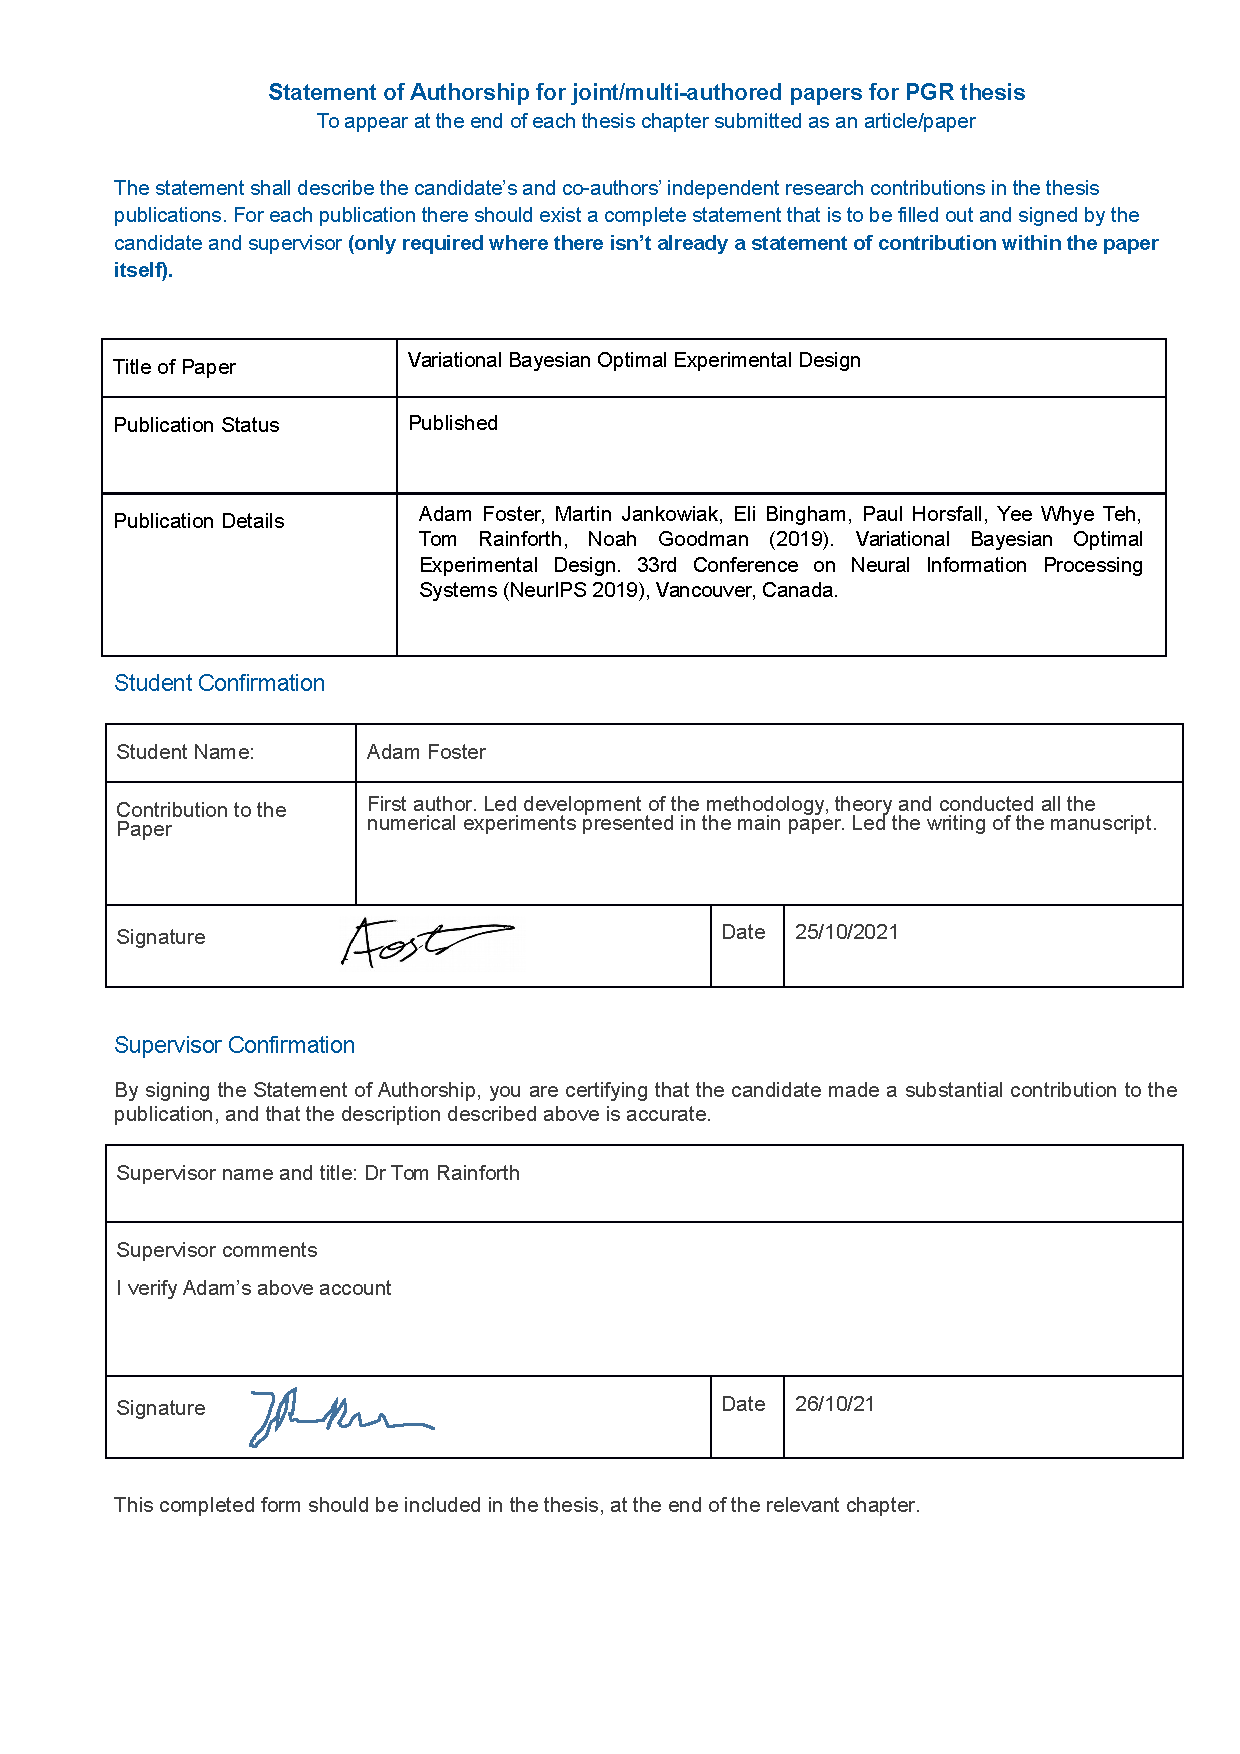
\includepdf[pagecommand={}, pages=-, trim=0mm 0mm 0mm 0mm, clip]{statementofauthorshipvboed.pdf}
	
	\chapter{A Unified Stochastic Gradient Approach to Designing Bayesian-Optimal Experiments}
	\label{chap:sgboed}
	This paper was published as the following
	\begin{quote}
		Adam Foster, Martin Jankowiak, Matthew O'Meara, Yee Whye Teh, and Thomas Rainforth. A Unified Stochastic Gradient Approach to Designing Bayesian-Optimal Experiments.  In \emph{Proceedings of the Twenty Third International Conference on Artificial Intelligence and Statistics}, pages 2959--2969. PMLR, 2020.
	\end{quote}
	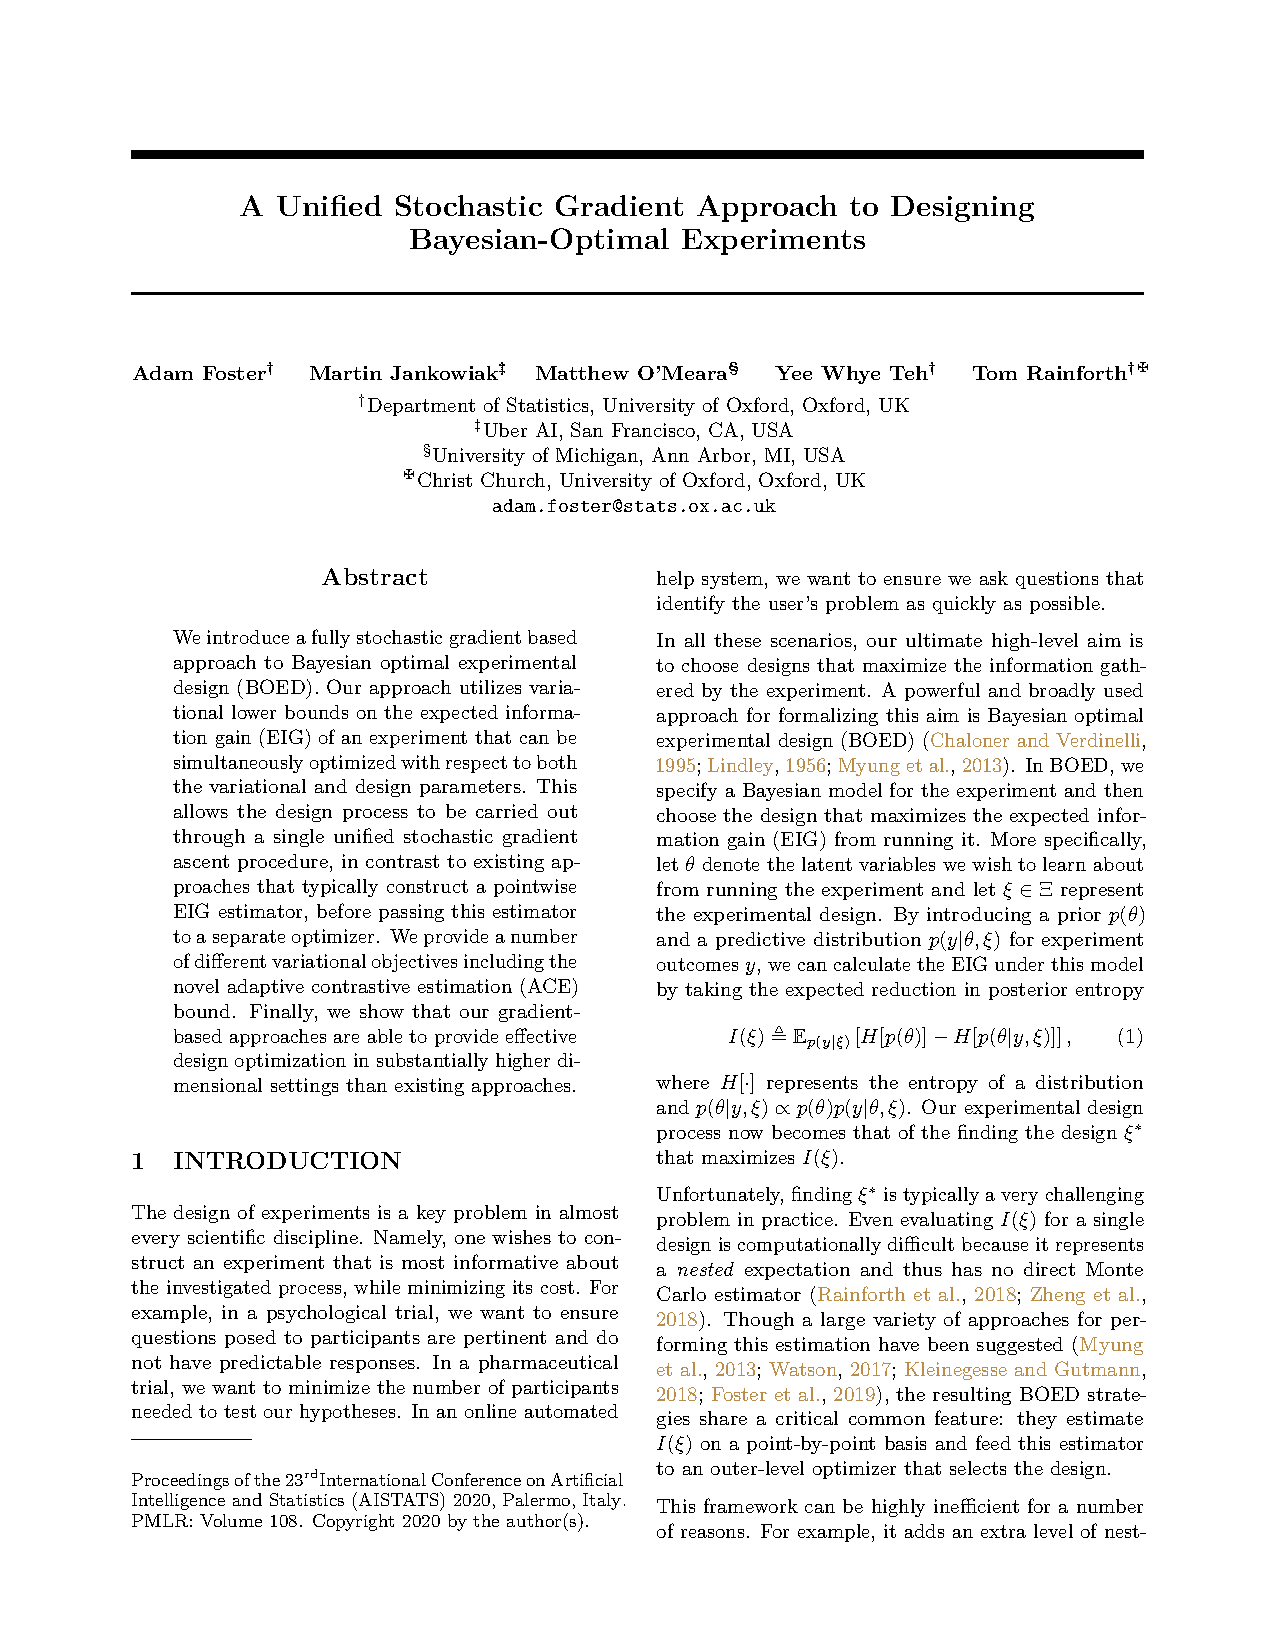
\includepdf[pagecommand={}, pages=-, trim=0mm 16.5mm 0mm 16.5mm, clip]{sgboed.pdf}
	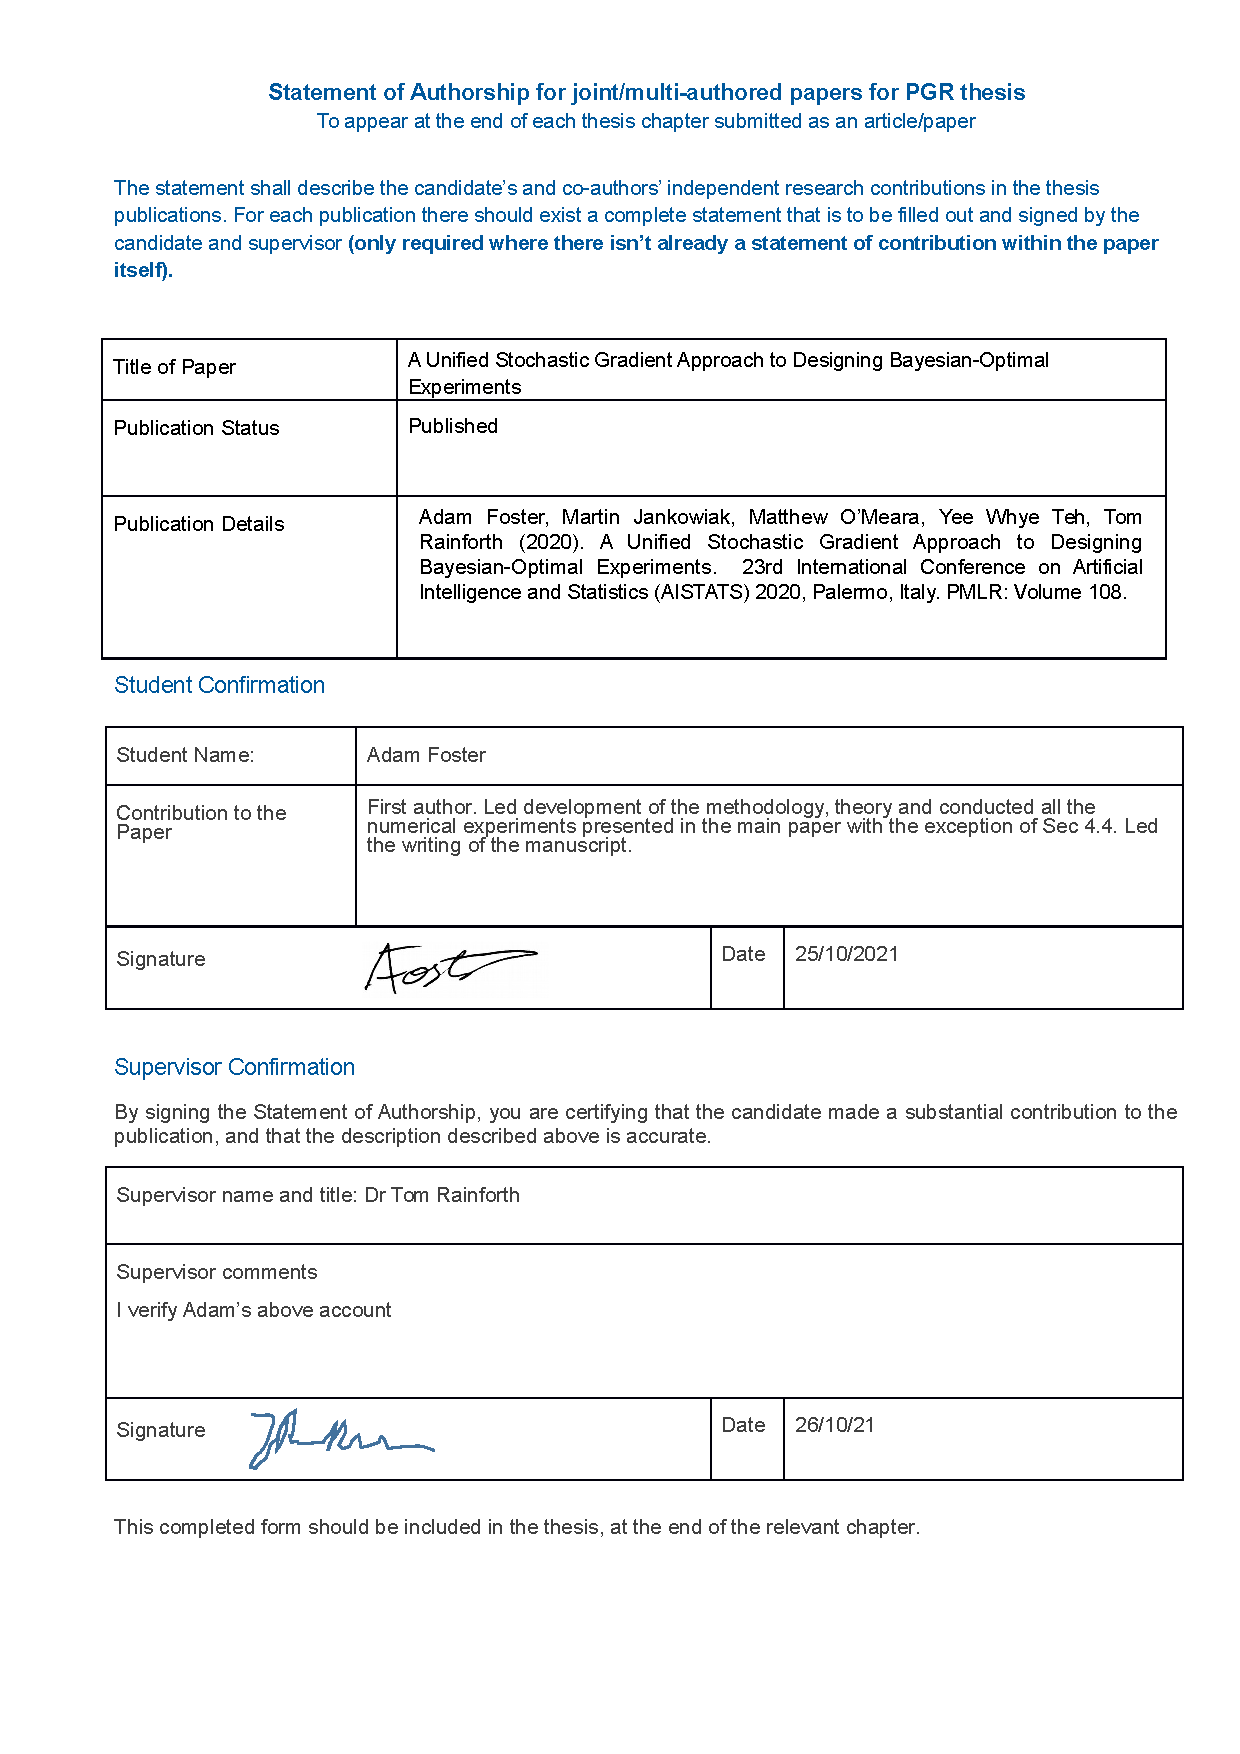
\includepdf[pagecommand={}, pages=-, trim=0mm 0mm 0mm 0mm, clip]{statementofauthorshipsgboed.pdf}
	
	\chapter{Unbiased MLMC stochastic gradient-based optimization of Bayesian experimental designs}
	\label{chap:mlmc}
	This paper was published as the following
	\begin{quote}
		Takashi Goda, Tomohiko Hironaka, Wataru Kitade and Adam Foster. Unbiased MLMC Stochastic Gradient-Based Optimization of Bayesian Experimental Designs. In \emph{SIAM Journal on Scientific Computing} vol. 44, pages A286--A311. SIAM, 2022.
	\end{quote}
	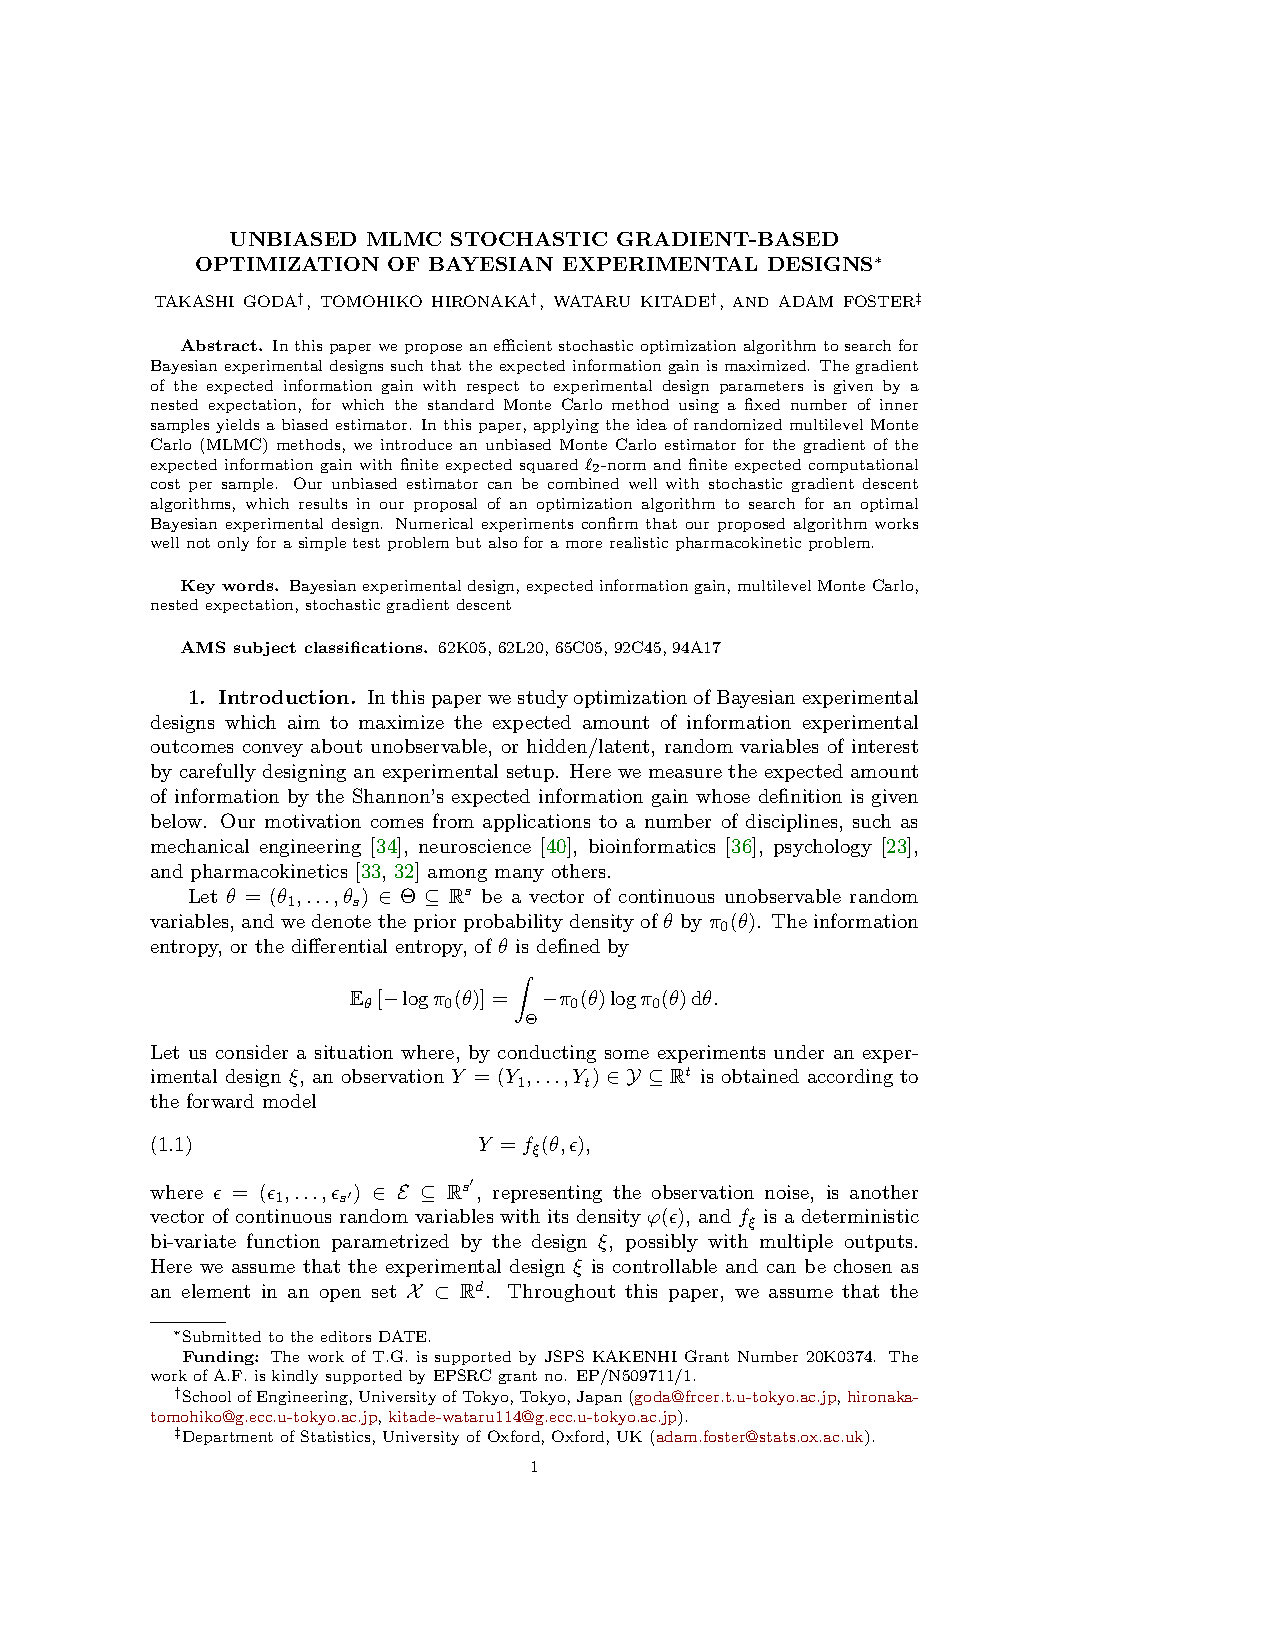
\includepdf[pagecommand={}, pages=-, trim=0mm 33mm 32mm 30mm, clip]{mlmc.pdf}
	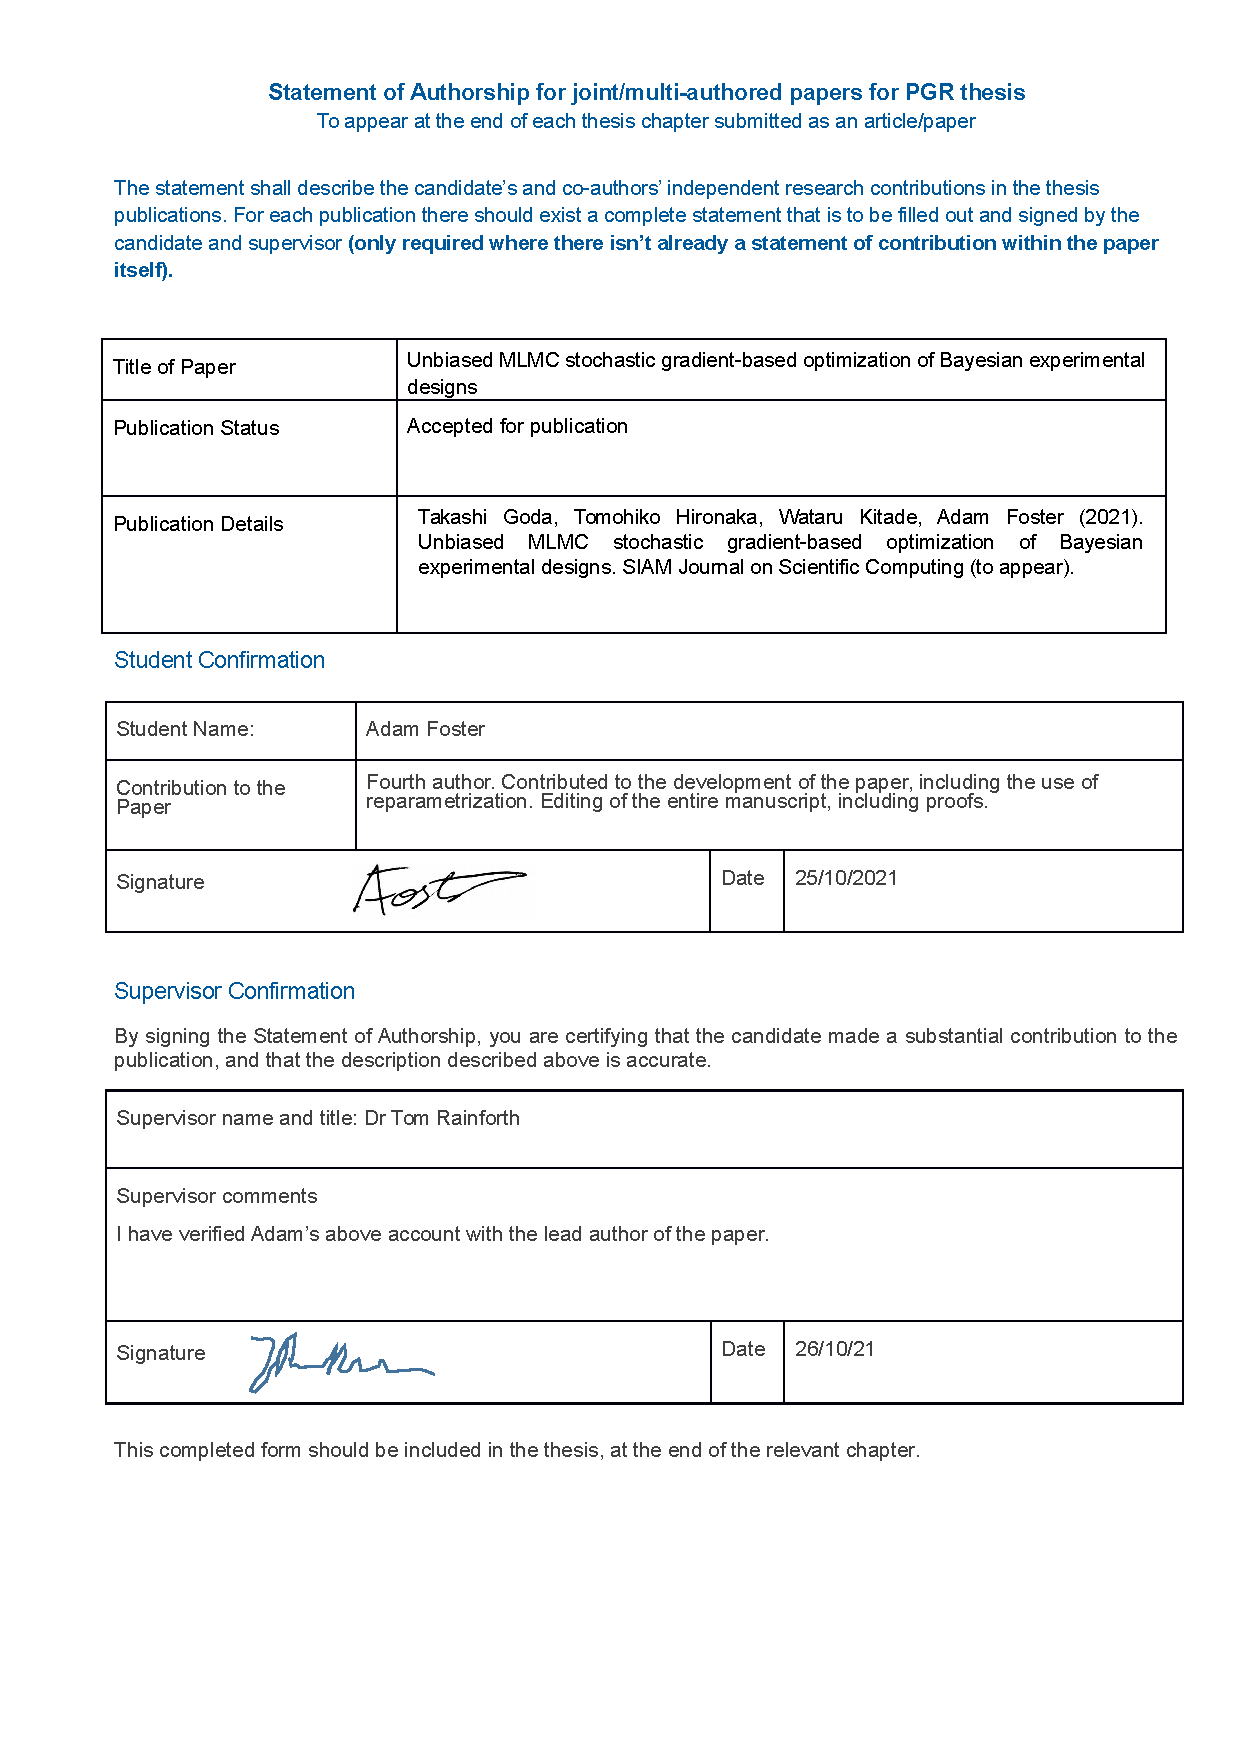
\includepdf[pagecommand={}, pages=-, trim=0mm 0mm 0mm 0mm, clip]{statementofauthorshipmlmc.pdf}
	
	\chapter{Deep Adaptive Design: Amortizing Bayesian Experimental Design}
	\label{chap:dad}
	This paper was published as the following
	\begin{quote}
		Adam Foster, Desi R Ivanova, Ilyas Malik, and Thomas Rainforth. Deep Adaptive Design: Amortizing Sequential Bayesian Experimental Design. In \emph{Proceedings of the 38th International Conference on Machine Learning}, pages 3384--3395. PMLR, 2021.
	\end{quote}
	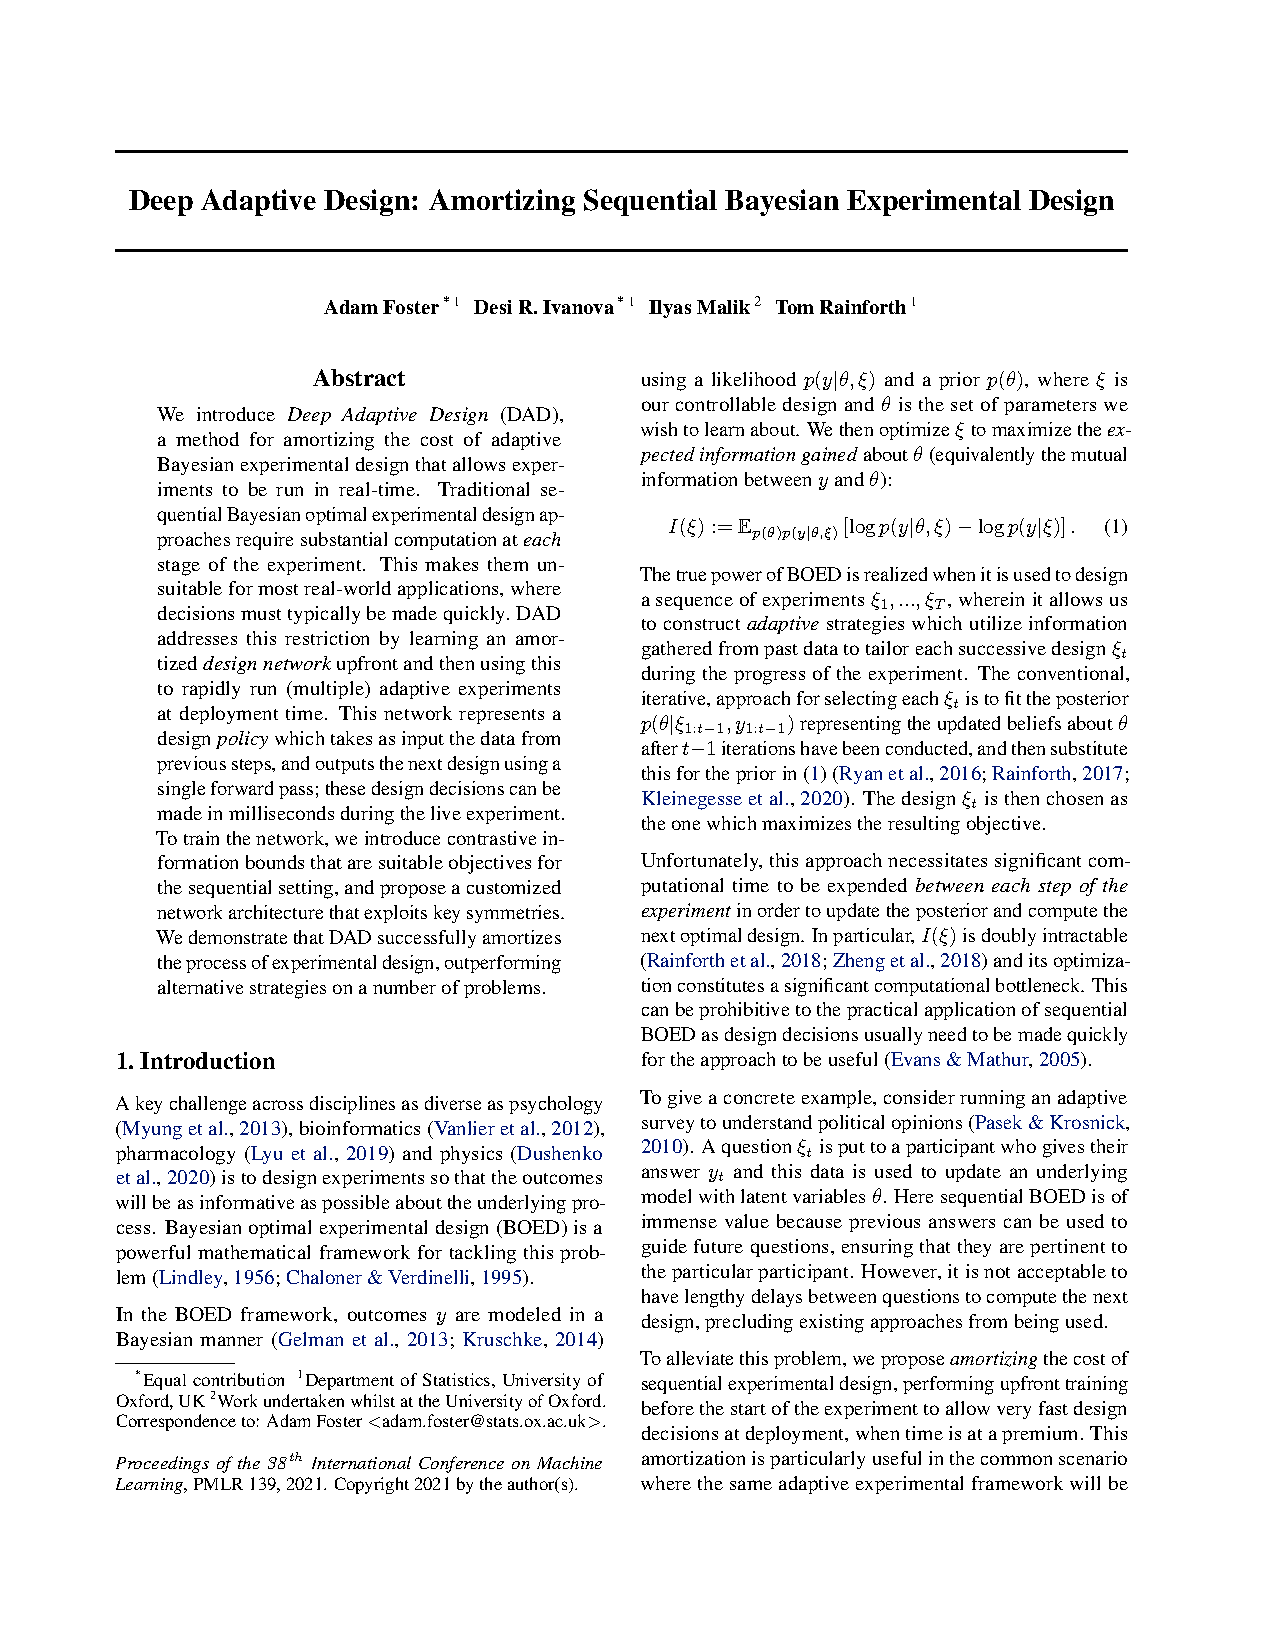
\includepdf[pagecommand={}, pages=-, trim=0mm 17mm 0mm 17mm, clip]{dad.pdf}
	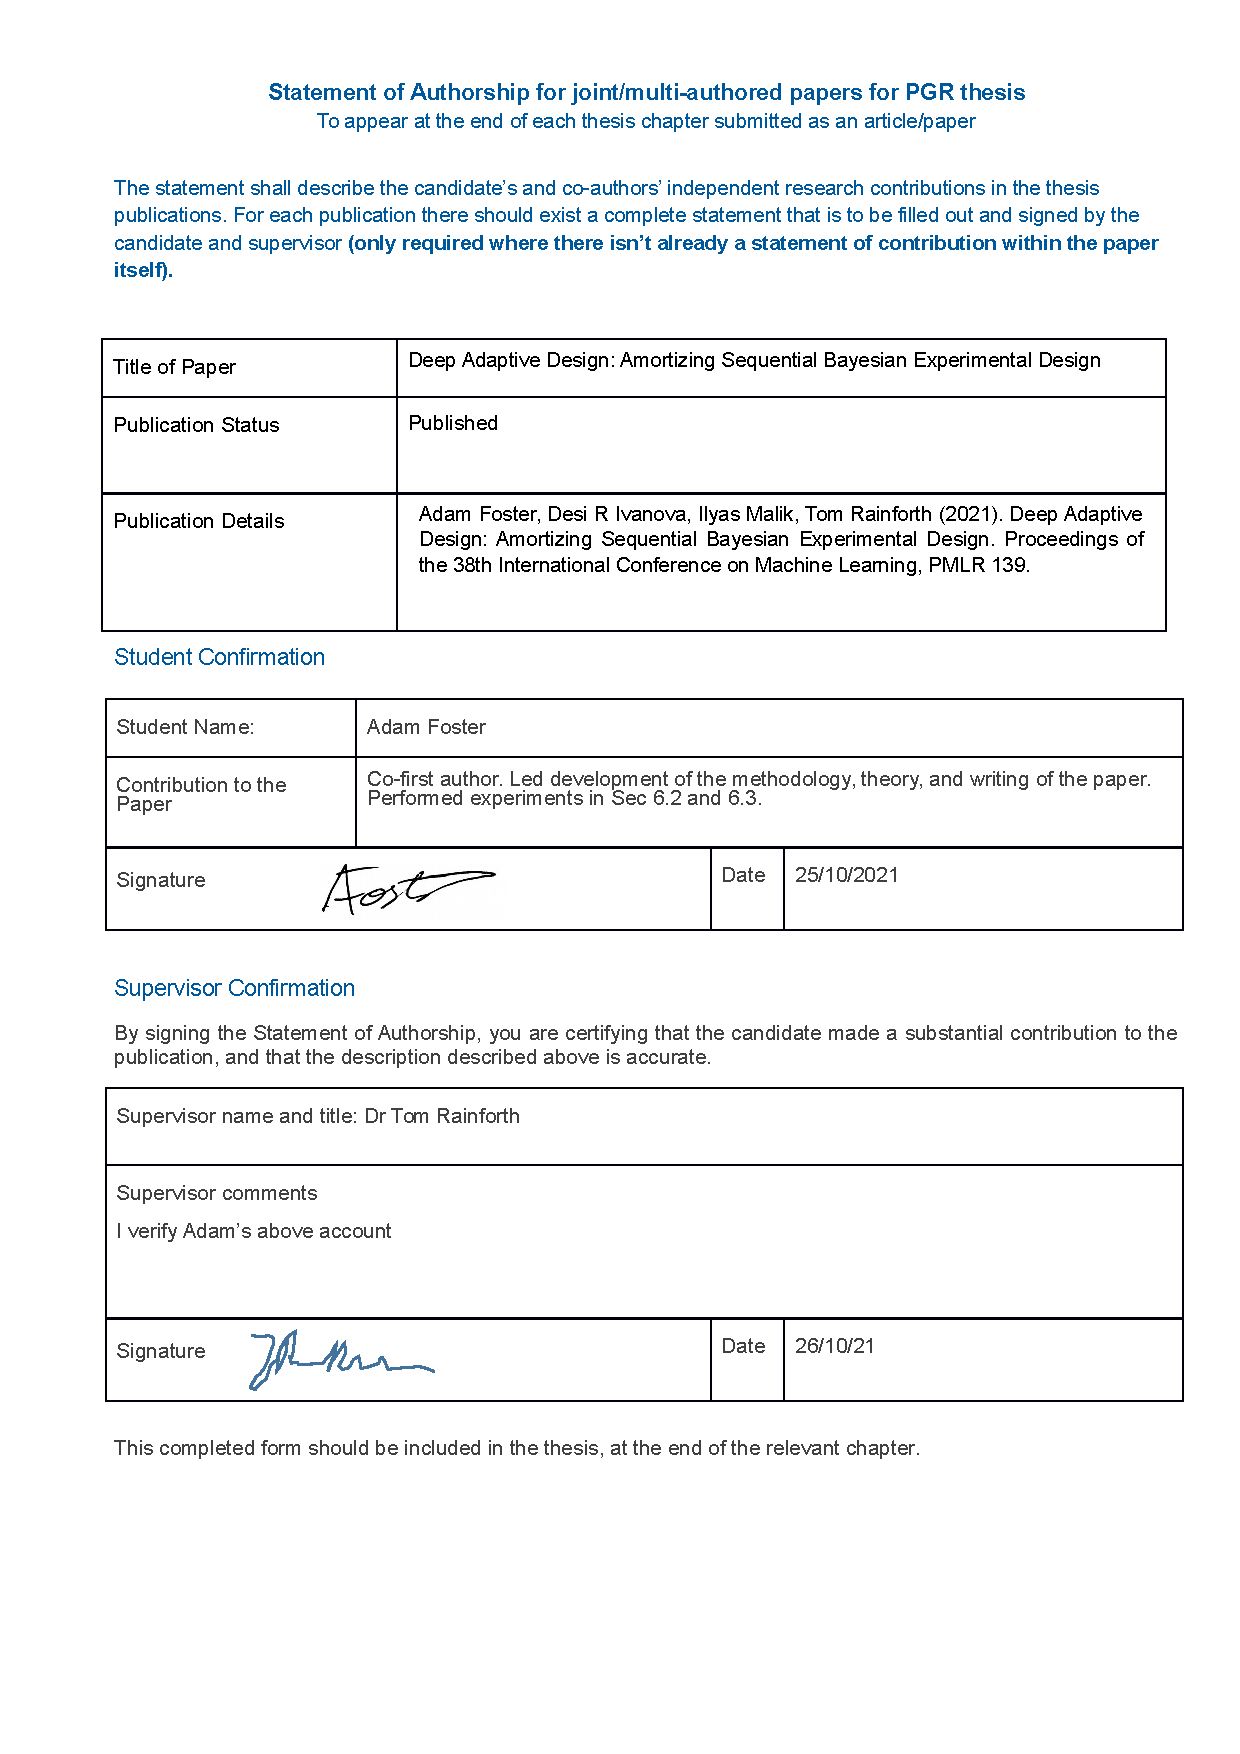
\includepdf[pagecommand={}, pages=-, trim=0mm 0mm 0mm 0mm, clip]{statementofauthorshipdad.pdf}
	
	\chapter{Implicit Deep Adaptive Design: Policy-Based Experimental Design without Likelihoods}
	\label{chap:idad}
	This paper was published as the following
	\begin{quote}
		Desi R Ivanova, Adam Foster, Steven Kleinegesse, Michael U Gutmann, Thomas Rainforth. Implicit Deep Adaptive Design: Policy-Based Experimental Design without Likelihoods. In \emph{Proceedings of the Thirty-fifth Conference on Neural Information Processing Systems}. Curran Associates, Inc., 2021.
	\end{quote}
	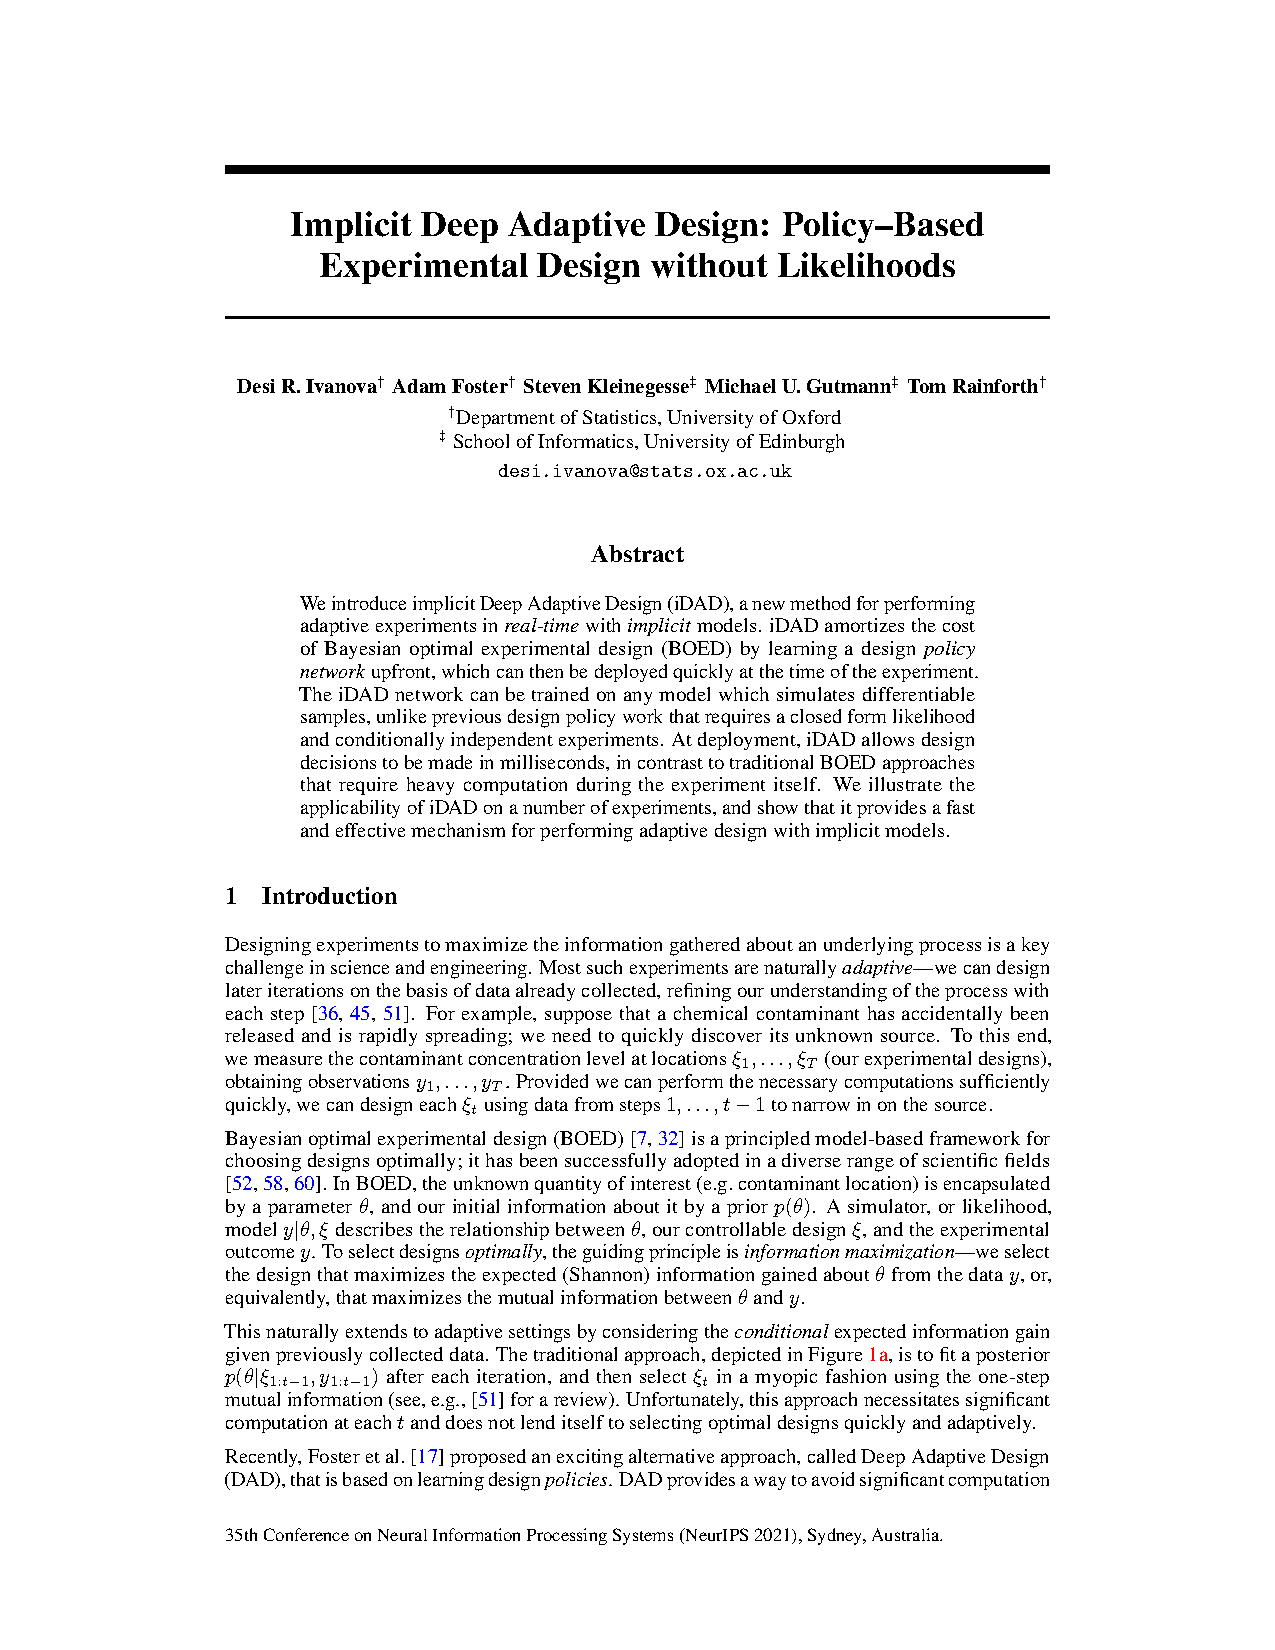
\includepdf[pagecommand={}, pages=-, trim=5mm 17.5mm 5mm 17.5mm, clip]{idad.pdf}
	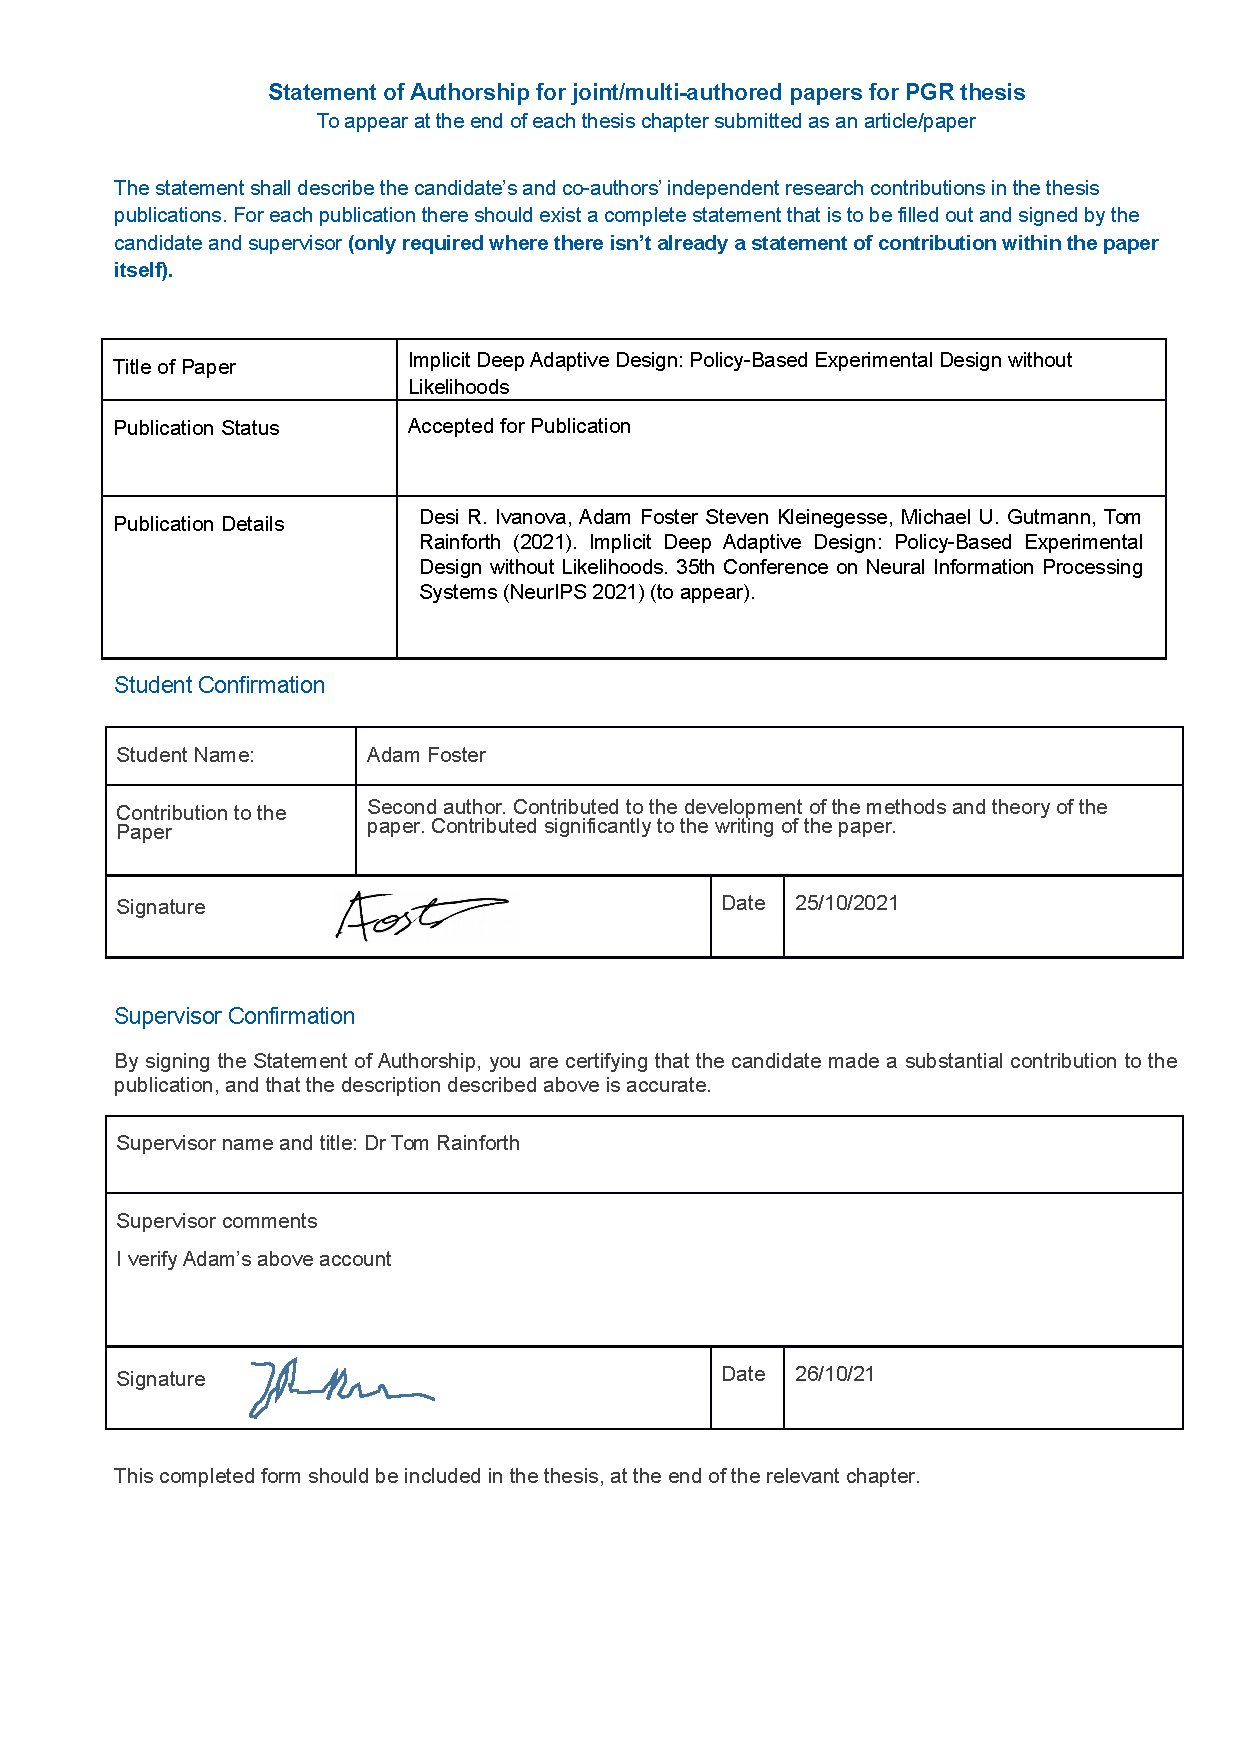
\includepdf[pagecommand={}, pages=-, trim=0mm 0mm 0mm 0mm, clip]{statementofauthorshipidad.pdf}
	
	\chapter{Discussion}
	\label{chap:discussion}
	This discussion is broken into a number of self-contained essays that delve into specific aspects of the concepts laid out in the earlier chapters.
	In Section~\ref{sec:modelselection}, we focus on elucidating the ideas of Chapters~\ref{chap:vboed} and~\ref{chap:sgboed} by focusing on the specific example use case of Bayesian \emph{model selection}. We examine how the variational estimators of Chapter~\ref{chap:vboed} look in this example, highlighting connections to other work, we also note how the approach of Chapter~\ref{chap:sgboed} translates to this specific case.
	In Section~\ref{sec:balessay}, we focus on comparing our work, particularly the estimators of Chapter~\ref{chap:sgboed} to work in the field of Bayesian active learning, drawing out the deep connections between experimental design and active learning.
	In Section~\ref{sec:brlessay}, we draw another connection, this time between the sequential experiment methods in Chapters~\ref{chap:dad} and~\ref{chap:idad} and the field of Bayesian reinforcement learning. We show that reinforcement learning provides a natural language to express the sequential experimental design problem.
	In Section~\ref{sec:estimators}, we investigate some of the statistical properties of various estimators discussed in this thesis. We focus on the NMC estimator, the PCE estimator introduced in Chapter~\ref{chap:sgboed}. We connect these more basic estimators with MLMC estimators, creating a stronger connection between earlier chapters and Chapter~\ref{chap:mlmc}.
	In Section~\ref{sec:bounds}, we present new results on mutual information bounds. This can be seen a generalising theory for some of the bounds derived in Chapters~\ref{chap:vboed}, \ref{chap:sgboed}, \ref{chap:dad} and \ref{chap:idad}.
	We conclude with a discussion of limitations of our work in Section~\ref{sec:limitations}.

	
	%%%%%%%%%%%%%%%%%%%%%%%%%%%%%%%%%%%%%%%%%%%%%%%%%%%%%%%%%%%%%%%%%%%%%%%%%%%%%%%%%%%%%%%%%%%%%%%%%%%%%
	% ESSAY ONE MODEL SELECTION
	%%%%%%%%%%%%%%%%%%%%%%%%%%%%%%%%%%%%%%%%%%%%%%%%%%%%%%%%%%%%%%%%%%%%%%%%%%%%%%%%%%%%%%%%%%%%%%%%%%%%%%
	\clearpage
	\section{Bayesian experimental design for model selection: variational and classification approaches}
	\label{sec:modelselection}
	
	\subsection{Introduction}
	Bayesian experimental design for model selection is a important and well-studied problem \citep{cavagnaro2010adaptive,vanlier2014optimal,hainy2018optimal}.
	In this essay, we tackle two questions that are relevant to this problem. First, how do recently proposed variational methods for experimental design \citep{foster2019variational,foster2020unified} translate into the model selection context? 
	% This is therefore something of a case study for these methods. 
	Second, how do these methods intersect with recently proposed classification-driven approaches to experimental design for model selection \citep{hainy2018optimal}?
	
	We begin by elucidating the key features of the model selection problem---it turns out that we can characterise the set-up as a semi-implicit model with a discrete latent variable of interest.
	The posterior or Barber--Agakov approach of \citet{foster2019variational} involves training an amortised inference network from data simulated from the model. We find that, for model selection, this network is exactly a (neural) classifier that predicts the true model that synthesised an observation from that synthetic experimental observation.
	The marginal + likelihood method of \citet{foster2019variational} also translates into the model selection case. 
	This method involves variational density estimation of experimental outcomes for each possible model.
	In other words, it involves approximating the model evidence of the data for each possible model.
	Finally, we examine how the stochastic gradient design approach of \citet{foster2020unified} applies here.
	This approach can build off the back of the Barber--Agakov bound, so it also utilises a classifier.
	The key difference here is that we differentiate the classifier output with respect to its input to learn the design at the same time as the classifier network parameters. This bears some similarities with adversarial approaches to neural network robustness \citep{carlini2019evaluating}.
	Finally, we compare and contrast the variational approach with other classification driven approaches in the literature.
	
	\subsection{Characterising the problem}
	We denote experimental designs by $\xi$ and experimental observations as $y$.
	Suppose there are $K$ competing models $\{m_1,\dots,m_k\}$ and we have a prior distribution $p(m)$ on which model we think is likely to  be correct.
	Given the choice of model, there are other model parameters $\psi \sim p(\psi|m)$.
	Conditional on the model, and on its parameters, we have a likelihood for the experiment $p(y|m,\psi,\xi)$ which we assume is known in closed form.
	
	One important feature of the model selection problem is that we do \emph{not} have a likelihood that directly relates the design $\xi$, observation $y$ and the latent variable of interest $m$. Instead, we have to account for the auxiliary latent variable $\psi$. 
	Indeed, we actually have $p(y|m,\xi) = \int_\Psi p(y|m,\psi,\xi) p(\psi|m) d\psi$.
	This case, where we have a closed form likelihood but for a larger set of variable, is referred to as a \emph{semi-implicit} model.
	
	In this essay, we focus on experimental design with the expected information gain (EIG) criterion, also called mutual information utility, that aims to reduce Shannon entropy in our beliefs about $m$. The EIG-optimal design is specifically,
	\begin{equation}
	\xi^* = \argmax_{\xi} \E_{p(m)p(\psi|m)p(y|m,\psi,\xi)}\left[ \log \frac{p(m|y,\xi)}{p(m)} \right].
	\end{equation}
	Finding $\xi^*$ amounts to estimating the EIG objective function and optimising over the space of possible designs.
	
	If we have already observed some data $\mathcal{D}=\{(\xi_1,y_1),\dots,(\xi_T,y_T)\}$, then we fit model-specific posteriors for the auxiliary variable $\psi$ for each model $p(\psi|m,\mathcal{D})$, and we compute the posterior over models $p(m|\mathcal{D}) \propto p(m)p(\mathcal{D}|m)$.
	Thus, we update our priors $p(m)$ and $p(\psi|m)$ on the basis of past data.
	
	\subsection{The variational approach}
	\subsubsection{Posterior lower bound}
	\citet{foster2019variational} considered variational estimation of the EIG. Their general strategy was to optimise variational upper or lower bounds on the EIG.
	Their simplest bound was the posterior lower bound  (also called the Barber--Agakov bound after \citet{ba}).
	With the variables we have in this model, the bound would be expressed as
	\begin{equation}
	\E_{p(m)p(\psi|m)p(y|m,\psi,\xi)}\left[ \log \frac{p(m|y,\xi)}{p(m)} \right] \ge \E_{p(m)p(\psi|m)p(y|m,\psi,\xi)}\left[ \log \frac{q_\phi(m|y)}{p(m)} \right].
	\end{equation}
	The new term $q_\phi(m|y,\xi)$ was generically referred to as the \emph{amortised approximate posterior} with variational parameters $\phi$. It is an approximate posterior distribution on the latent variable $m$ of interest. The amortisation here refers to the fact that we learn a function from $y$ to a distribution over $m$ (for different $\xi$, we would train separate functions).
	For the model selection approach, then, $q_\phi$ is a function from $y$ to a distribution over the discrete model indicator $m$.
	First, since $m$ is discrete, the choice of variational family is moot, because every distribution over $m$ can be finitely represented.
	Second, $q_\phi$ has a very simple interpretation. It is a classifier that attempts to predict, on the basis of input $y$, which model of $m_1,\dots,m_k$ generated that data, specifically trying to estimate the posterior probability $p(m|y,\xi)$ over the $k$ different possibilities for $m$.
	Importantly though, rather than just attempting to predict the correct model that was responsible for generating the data $y$, it is essential that we have a \emph{probabilistic} classifier that assigns probabilities to each possible model. 
	For this probabilistic classifier, the issue of calibration becomes central, as we hope that our classifier probabilities will approach $p(m|y,\xi)$ during training.
	
	We have established that $q_\phi$ is simply a probabilistic classifier for the model selection case.
	How should this classifier be trained? 
	In general, \citet{foster2019variational} proposed training $q_\phi$ by stochastic gradient methods \citep{robbins1951stochastic,kingma2014adam} to maximise the lower bound with respect to $\phi$
	\begin{equation}
	\phi^* = \argmax_\phi \E_{p(m)p(\psi|m)p(y|m,\psi,\xi)}\left[ \log \frac{q_\phi(m|y)}{p(m)} \right]
	\end{equation}
	In model selection, training $\phi$ simply means training the parameters of the classifier. 
	Maximising the posterior lower bound is equivalent to simply maximising the expected log likelihood under $q$, i.e. 
	\begin{equation}
	\phi^* = \argmax_\phi \E_{p(m)p(\psi|m)p(y|m,\psi,\xi)}\left[ \log q_\phi(m|y) \right].
	\end{equation}
	This is true because $p(m)$ has no dependence on $\phi$.
	So, we see that training $q_\phi$ to maximise the variational posterior lower bound amounts to maximum likelihood training of a neural classifier when we are in the setting of model selection.
	(Care may be needed to ensure the classifier produces good \emph{probabilistic uncertainty}, as well as getting good predictions, as these probabilities are central to our method.)
	
	In fact, we have an enhanced setting in which we can draw an infinite amount of training data by simulating from $p(m)p(\psi|m)p(y|m,\psi,\xi)$.
	To do this, we sample a random model $m$ from its prior, then a random set of parameters $\psi \sim p(\psi|m)$ for the chosen model, and then simulate an experimental outcome under design $\xi$.
	Importantly, we do not need to draw a fixed training or test set, and we never need to show the classifier the same examples twice, we instead draw new batches on the fly.
	One particularly important consequence of this is that the spectre of \emph{over-fitting} is much reduced in our case, as there is no fixed training set to overfit to.
	
	We now see another important point---the negative log-likelihood loss of the classifier is essentially an estimate of the EIG, up to a constant.
	Suppose we have completed training and reached parameters $\hat{\phi}$.
	Then the EIG estimate is
	\begin{equation}
	\text{EIG}(\xi) \approx \E_{p(m)p(\psi|m)p(y|m,\psi,\xi)}\left[ \log \frac{q_{\hat{\phi}}(m|y)}{p(m)} \right] = \E_{p(m)p(\psi|m)p(y|m,\psi,\xi)}\left[ \log q_{\hat{\phi}}(m|y) \right] + H[p(m)]
	\end{equation}
	and we can estimate the expectation with new, independent batches simulated from the model.
	
	In summary, the posterior lower bound method for model selection amounts to training a classifier on (infinite) simulated data to predict $m$ from $y$. The optimal design $\xi^*$ will be approximated by the classifier which has the best (lowest) validation loss, which is a good approximation of having the highest EIG.
	
	
	\subsubsection{Marginal + likelihood estimator}
	The posterior lower bound is not the only way to estimate the EIG proposed by \citet{foster2019variational}.
	Both the marginal and the VNMC methods require an explicit likelihood, so they are not suitable for the semi-implicit model selection scenario.
	The marginal + likelihood estimator is
	\begin{equation}
	\text{EIG}(\xi) \approx \E_{p(m)p(\psi|m)p(y|m,\psi,\xi)}\left[ \log \frac{q_\ell(y|m,\xi)}{q_p(y|\xi)} \right].
	\end{equation}
	This estimator translates, with some simplification, into the model selection setting. 
	The `approximate likelihood' $q_\ell(y|m,\xi)$ in the model selection setting is an approximation of the model evidence $q_\ell(y|m,\xi) \approx p(y|m,\xi)$.
	For model selection when $m$ is discrete, we do not need to separately estimate $q_p$ and $q_\ell$, we can instead sum over $m$ to obtain
	\begin{equation}
	q_p(y|\xi) = \sum_m p(m) q_\ell(y|m,\xi).
	\end{equation}
	As shown in Appendix A.4 of \citet{foster2019variational}, the estimator actually becomes a lower bound 
	\begin{equation}
	\label{eq:model_selection_bound}
	\text{EIG}(\xi) \ge \E_{p(m)p(\psi|m)p(y|m,\psi,\xi)}\left[ \log \frac{q_\ell(y|m,\xi)}{\sum_{m'} p(m') q_\ell(y|m'	,\xi)} \right]
	\end{equation}
	on the EIG in this case, which is not generally the case for the marginal + likelihood method.
	(In fact, this lower bound is itself a special case of the likelihood-free ACE lower bound introduced in \citet{foster2020unified}. Indeed, if we take the prior as the variational posterior and let $L\to\infty$ in the LF-ACE bound, we recover this lower bound.)
	
	This lower bound also has a nice interpretation in the model selection scenario. The best design will be the one where the lower bound is largest, which happens, loosely speaking, when $q_\ell(y|m,\xi)$ is much larger than $\sum_m p(m) q_\ell(y|m,\xi)$. That means the approximate model evidence for the observation $y$ under the correct model $m$ is much larger than its evidence under other models. Thus, using the experiment with design $\xi$ and observing $y$ will allow us to easily discriminate between models.
	
	To explicitly use this method, we need to choose trainable density estimators for $q_\ell(y|m,\xi; \phi)$ with parameters $\phi$.
	The simplest method would be to have a distinct set of variational parameters for each value of $m$ and $\xi$.
	Whilst it is possible to use a Gaussian density model, we could use more sophisticated methods such as normalising flows \citep{rezende2015variational}. The training approach is similar to that for the posterior method.
	We use infinite simulated data, and maximise the variational lower bound using stochastic gradient optimisers.
	
	
	The last two sections highlight a general feature of the variational methods of \citet{foster2019variational}---we can either make variational approximations to densities over $m$ or over $y$. Both lead to valid bounds.
	
	\subsection{Stochastic gradient optimisation of the design}
	So far, we have focused on variational estimation of the EIG.
	As shown in \citet{foster2020unified}, it is only a short jump from variational estimation of the EIG to stochastic gradient optimisation of the design using a variational lower bound on EIG.
	The benefit here, of course, is that we do not have conduct a grid search, co-ordinate exchange or similar algorithm over the design space.
	What we require instead is a continuous design space and the ability to differentiate observations with respect to designs.
	
	Whilst \citet{foster2020unified} focused on explicit likelihood models, both the posterior (Barber--Agakov) lower bound and the LF-ACE bound are applicable to the semi-implicit model selection setting. There is just one thing to check, which is that we can compute a derivative $\partial y/\partial \xi$.
	In the semi-implicit case, this is often fine. For example, if $p(y|m,\psi,\xi)$ takes the form $y = g(m,\psi,\xi,\epsilon)$ for a differentiable $g$ and an independent noise random variable $\epsilon$.
	
	Assuming this is the case, we can train $\xi$ by stochastic gradient using either the posterior bound or the simplified LF-ACE bound that was derived in \eqref{eq:model_selection_bound}.
	We focus on the posterior lower bound for simplicity.
	Recall that, for the posterior bound, we are training a classifier to predict $m$ from $y$.
	We have
	\begin{equation}
	\text{EIG}(\xi) \ge \E_{p(m)p(\psi|m)p(y|m,\psi,\xi)}\left[ \log q_\phi(m|y) \right] + H[p(m)]
	\end{equation}
	where $q_\phi$ is the classifier.
	One thing that we skimmed over slightly in the previous section was that $\phi$ implicitly depends on $\xi$ via the training data, and different $\xi$ will have different classifiers with different optimal values of the classifier parameters $\phi$.
	
	In \citet{foster2020unified}, rather than training separate classifiers with different designs $\xi$, we update $\xi$ and $\phi$ togther in one stochastic gradient optimisation over the combined set of variables $(\xi,\phi)$.
	To explicitly write down the $\xi$ gradient here, let's assume that we do have $y = g(m,\psi,\xi,\epsilon)$, so we can write
	\begin{equation}
	\mathcal{L}(\xi,\phi) = \E_{p(m)p(\psi|m)p(\epsilon)}\left[ \log q_\phi(m|g(m,\psi,\xi,\epsilon)) \right] + H[p(m)].
	\end{equation}
	In this form, the $\xi$ gradient can be simply calculated as
	\begin{equation}
	\label{eq:grad}
	\frac{\partial \mathcal{L}}{\partial \xi} = \E_{p(m)p(\psi|m)p(\epsilon)}\left[ \left.\frac{\partial \log q_\phi}{\partial y}\right\vert_{m,g(m,\psi,\xi,\epsilon)}\left.\frac{\partial g}{\partial \xi}\right\vert_{m,\psi,\xi,\epsilon} \right].
	\end{equation}
	The beauty of modern auto-diff frameworks, of course, means that we do not even need to calculate this explicitly ourselves.
	
	For model selection, \eqref{eq:grad} has a natural interpretation. 
	We want to increase the lower bound $\mathcal{L}$ by moving to regions in which the classifier can confidently predict the correct model label $m$. This corresponds to moving $y$ into regions in which $\log q_\phi(m|y)$ is larger \emph{for the model that actually generated $y$}.
	In other words, we want the input to the classifier $y$ to be pushed to regions where the classifier already finds it easy to classify correctly.
	That is, regions where deciding which model is correct is easier.
	We then exploit the differentiable relationship between $\xi$ and $y$, and use this signal to `improve' the input to the classifier by adjusting the design $\xi$ to that such datasets $y$ are more likely to be synthesised.
	
	At the same time, we are constantly making gradient updates on the classifier parameters $\phi$. This means that, as the distribution of $(m,y)$ changes, the classifier can adjust accordingly.
	
	If this sounds dubious, it is worth taking a step back. We are quite simply optimising the lower bound $\mathcal{L}(\xi,\phi)$ jointly with respect to $\xi$ and $\phi$, in the hopes that this global maximum may closely correspond to the EIG maximiser $\xi^*$.
	We actually have a guarantee that the value of $\mathcal{L}$ at our final trained variables $\hat{\xi},\hat{\phi}$ is a lower bound on $\text{EIG}(\hat{\xi})$, i.e.~the true value of $\hat{\xi}$ cannot be worse than the value we estimate for it.
	
	Whilst the method is approximate, because we cannot quantify the discrepancy between $\mathcal{L}$ and the true EIG, it is highly scalable to very large design spaces. Other bounds presented in \citet{foster2020unified} have the added benefit that they become equal to the EIG in a limit, providing some assurances that the global maximum of $\mathcal{L}$ is a good design.
	\citet{foster2020unified} also introduced the evaluation method of establishing \emph{lower and upper} bounds on chosen designs. This numerically bounds the discrepancy between the training objective $\mathcal{L}$ and the true EIG objective. Sadly, the upper bounds are only valid for explicit likelihood models; they don't work in the semi-implicit model selection case.
	
	Finally, all of the above discussion carries over if we were to use the lower bound of \eqref{eq:model_selection_bound} instead of the posterior bound.
	
	\subsection{Comparing with other classification approaches}
	We have established that the variational posterior approach of \citet{foster2019variational} instructs us to learn a classifier to predict $m$ from $y$ and use the log probabilities $q_\phi(m|y)$ to estimate EIG.
	Other authors have considered supervised classification as a means to perform Bayesian experimental design for model selection.
	
	Here, we focus on \citet{hainy2018optimal}, which is ``the first approach using supervised learning methods for optimal Bayesian design.''
	This method trains a classifier that predicts $m$ using $y$, with separate classifiers for different $\xi$.
	They focus on training decision trees and random forest classifiers \citep{breiman2001random}.
	Since random forests are not generally trained by stochastic gradient methods, this means that they fall back on simulating fixed training and test datasets of samples $(m_j, y_j)_{j=1}^J$ from $p(m)p(\psi|m)p(y|m,\psi,\xi)$.
	The training dataset is used to train the classifier model, whilst the test dataset gives unbiased estimates of the posterior loss.
	There is a danger that the classifier may overfit to the training set in this case.
	Compare this with the training of stochastic gradient classifiers in our previous sections---here we can draw fresh training batches on the fly, and avoid overfitting to a training set.
	
	Decision trees and random forests do provide estimates of the class probabilities $q(m|y)$, but they are relatively noisy.
	For this reason, \citet{hainy2018optimal} focus on the 0--1 loss to evaluate designs.
	In the language of classification, therefore, they choose the design which gives the best \emph{test accuracy}.
	Again, this is different to the variational approach which fits a neural classifier that automatically provides smooth probability estimates $q_\phi(m|y)$.
	The latter case was applied to estimate the information gain, which we showed is equivalent to choosing the design which gives the best \emph{test loss}, assuming a negative log-likelihood loss function.
	
	The trade-offs between these methods are clear when we consider optimising over a large design space.
	For the variational method, we have to train a number of neural networks to convergence. For the classification approach of \citet{hainy2018optimal}, we train a number of random forest classifiers---this may be significantly more computationally efficient.
	\citet{hainy2018optimal} propose embedding their 0--1 loss estimation within a co-ordinate exchange algorithm \citep{meyer1995coordinate} to optimise over designs.
	The variational method, on the other hand, can naturally be embedded in a unified stochastic gradient optimisation to find the optimal design through stochastic gradient optimisation.
	The former may be more effective when the design space is not continuous, the latter can work well in a high-dimensional design space that is difficult to search using discrete methods.
	
	
	%%%%%%%%%%%%%%%%%%%%%%%%%%%%%%%%%%%%%%%%%%%%%%%%%%%%%%%%%%%%%%%%%%%%%%%%%%%%%%%%%%%%%%%%%%%%%%%%%%%%%
	% ESSAY TWO BAYESIAN ACTIVE LEARNING
	%%%%%%%%%%%%%%%%%%%%%%%%%%%%%%%%%%%%%%%%%%%%%%%%%%%%%%%%%%%%%%%%%%%%%%%%%%%%%%%%%%%%%%%%%%%%%%%%%%%%%%
	
	\clearpage
	\section{Bayesian active learning by disagreement and Bayesian experimental design}
	\label{sec:balessay}
	
	\subsection{Introduction}
	The purpose of this essay is to highlight the connection between the Bayesian Active Learning by Disagreement (BALD) score as estimated by \citet{gal2017deep} and the Prior Contrastive Estimation (PCE) bound of \citet{foster2020unified}.
	There is a deep connection between Bayesian experimental design and Bayesian active learning. 
	A significant touchpoint is the use of the mutual information score \citep{lindley1956}
	\begin{equation}
	\label{eq:info}
	I(\xi) = \E_{p(\theta)p(y|\theta,\xi)}\left[H[p(\theta)] - H[p(\theta|y,\xi)]\right].
	\end{equation}
	to acquire new information in a Bayesian model with parameters $\theta$ where, $y$ is the as yet unobserved outcome, and $\xi$ is the design to be chosen.
	
	%\section{Acquiring data using the mutual information score}
	%Choosing how and where to acquire new information is an age old problem in statistics and machine learning.
	%The seminal paper \citet{lindley1956} introduced the principle of information-based acquisition.
	%In a Bayesian model with parameters $\theta$, observation $y$ and designs $\xi$ through which to acquire new observations, the best design to choose is the one which most reduces the expected Shannon entropy of the posterior distribution over $\theta$. This is equivalent to choosing the design $\xi$ with the largest mutual information score
	%\begin{equation}
	%	\label{eq:info}
	%	I(\xi) = \E_{p(\theta)p(y|\theta,\xi)}\left[H[p(\theta)] - H[p(\theta|y,\xi)]\right].
	%\end{equation}
	%Whilst the mutual information score has a number of attractive theoretical properties, its use has been limited by the difficult of calculating the score $I(\xi)$.
	
	\subsection{Bayesian Active Learning by Disagreement}
	One of the computational challenges inherent in estimating \eqref{eq:info} directly is that it involves repeated estimation of posterior distributions $p(\theta|y,\xi)$ for different simulated observations $y$.
	To remove this particular bottleneck, \citet{houlsby2011bayesian} introduced a rewriting of the mutual information score using Bayes rule
	\begin{equation}
	\label{eq:bald}
	I(\xi) = H[p(y|\xi)] - \E_{p(\theta)}\left[ H[p(y|\theta,\xi)] \right].
	\end{equation}
	Whilst this is exactly equal to the original mutual information score, the new way of expressing $I$ removes the requirement to estimate posterior distributions over $\theta$.
	They termed \eqref{eq:bald} the Bayesian Active Learning by Disagreement (BALD) score.
	
	Unfortunately, the story does not end with the BALD score because it still typically involves some intractable computations that must be estimated.
	For example, \citet{houlsby2011bayesian} focused on approximations for Gaussian Process models \citep{williams2006gaussian}.
	
	The more recent work by \citet{gal2017deep} estimated the BALD score in the context of Bayesian deep learning classifiers.
	In such a model, $\theta$ represents the parameters of a classification model, and $p(y|\theta,\xi)$ is a probability distribution over classes $y\in\{c_1,\dots,c_k\}$. 
	Computing $p(y|\theta,\xi)$ involves a forward pass through the classifier with input $\xi$ and parameters $\theta$, the network generally ends in a softmax activation to produce a normalised distribution.
	To sample different values of $\theta$, \citet{gal2017deep} employed Monte Carlo Dropout \citep{gal2016dropout}.
	Given independent samples $\theta_1,\dots,\theta_M$ from $p(\theta)$, they proposed the following Deep BALD (DBALD) estimator of $I(\xi)$
	\begin{equation}
	I(\xi) \approx \hat{I}_\text{DBALD}(\xi) = H\left[ \frac{1}{M}\sum_{i=1}^M p(y|\theta_i,\xi) \right] - \frac{1}{M} \sum_{i=1}^M H[p(y|\theta_i,\xi)]
	\end{equation}
	where $H[P(y)] = -\sum_c P(y=c)\log P(y=c)$.
	
	\paragraph{Notation} For comparison with the original paper, we used $\theta$ in place of $\bm{\omega}$, $\xi$ in place of $\mathbf{x}$, $M$ in place of $T$ and $p(\theta)$ is used in place of $q^*_\theta(\bm{\omega})$.
	
	\subsection{Prior Contrastive Estimation}
	In the context of stochastic gradient optimisation of Bayesian experimental designs, \citet{foster2020unified} also considered the mutual information score $I(\xi)$ and the rearrangement \eqref{eq:bald}.
	They proved the following Prior Contrastive Estimation (PCE) lower bound on $I(\xi)$
	\begin{equation}
	I(\xi) \ge \E_{p(\theta_0)p(y|\theta_0,\xi)p(\theta_1)\dots p(\theta_L)}\left[ \log \frac{p(y|\theta_0,\xi)}{\frac{1}{L+1} \sum_{\ell=0}^L p(y|\theta_\ell,\xi)} \right]
	\end{equation}
	and used this bound to optimise $\xi$ by stochastic gradient.
	One approach to estimate this bound using finite samples is the estimator
	\begin{equation}
	\hat{I}_\text{PCE-naive}(\xi) = \frac{1}{M} \sum_{m=1}^M \log \frac{p(y_m|\theta_{m0},\xi)}{\frac{1}{L+1}\sum_{\ell=0}^L p(y_m|\theta_{m\ell},\xi)  }.
	\end{equation}
	where $y_m,\theta_{m0}\sim p(y,\theta|\xi)$ and $\theta_{m\ell}\sim p(\theta)$ for $\ell \ge 1$.
	However, we can also re-use samples more efficiently to give the estimator
	\begin{equation}
	\label{eq:pce}
	\hat{I}_\text{PCE}(\xi) = \frac{1}{M} \sum_{m=1}^M \log \frac{p(y_m|\theta_{m},\xi)}{\frac{1}{M}\sum_{\ell=1}^M p(y_m|\theta_{\ell},\xi)  }.
	\end{equation}
	where $y_m,\theta_m \sim p(y,\theta|\xi)$. (To check the expectation of this version matches the PCE bound with $L=M-1$, we simply move the $\E$ sign inside of the summation.)
	Finally, \citet{foster2020unified} discussed a speed-up that is possible when $y$ is a discrete random variable taking values in $\{ c_1,\dots,c_k \}$.
	In this case, we can integrate out $y$ by summing over it, rather than by drawing random samples of $y$.
	This method, called Rao-Blackwellisation, results in the estimator
	\begin{equation}
	\hat{I}_\text{PCE-RB}(\xi) = \frac{1}{M} \sum_{m=1}^M \sum_c p(y=c|\theta_m,\xi) \log \frac{p(y=c|\theta_{m},\xi)}{\frac{1}{M}\sum_{\ell=1}^M p(y=c|\theta_{\ell},\xi)  }.
	\end{equation}
	
	\subsection{PCE and DBALD equivalence}
	We have looked at two parallel ways of approximating $I(\xi)$.
	The interesting result is that \emph{the Rao-Blackwellised PCE estimator and the DBALD estimator are the same}.
	We can see this by direct calculation
	\begin{align}
	\hat{I}_\text{PCE-RB}(\xi) &= \frac{1}{M} \sum_{m=1}^M \sum_c p(y=c|\theta_m,\xi) \log \frac{p(y=c|\theta_{m},\xi)}{\frac{1}{M}\sum_{\ell=1}^M p(y=c|\theta_{\ell},\xi)  } \\
	\begin{split}&= \frac{1}{M} \sum_{m=1}^M \sum_c p(y=c|\theta_m,\xi) \log p(y=c|\theta_{m},\xi) \\
	& \qquad - \frac{1}{M} \sum_{m=1}^M \sum_c p(y=c|\theta_m,\xi) \log\left(\frac{1}{M}\sum_{\ell=1}^M p(y=c|\theta_{\ell},\xi)  \right) \end{split}\\
	&= -\frac{1}{M} \sum_{m=1}^M H[p(y|\theta_m,\xi)]  - \frac{1}{M} \sum_{m=1}^M \sum_c p(y=c|\theta_m,\xi) \log\left(\frac{1}{M}\sum_{\ell=1}^M p(y=c|\theta_{\ell},\xi)  \right)\\
	&= -\frac{1}{M} \sum_{m=1}^M H[p(y|\theta_m,\xi)]  - \sum_c \left(\frac{1}{M}  \sum_{m=1}^M  p(y=c|\theta_m,\xi) \right) \log\left(\frac{1}{M}\sum_{\ell=1}^M p(y=c|\theta_{\ell},\xi)  \right)\\
	&= -\frac{1}{M} \sum_{m=1}^M H[p(y|\theta_m,\xi)]  + H\left[\frac{1}{M}  \sum_{m=1}^M  p(y|\theta_m,\xi) \right]\\
	&= \hat{I}_\text{DBALD}(\xi).
	\end{align}
	A major consequence of this result is that \emph{the expectation of the DBALD score is a lower bound on the true mutual information score}.
	We also note that this estimator has been used by \citet{vincent2017} in the context of Bayesian experimental design, although they did not show that it was a stochastic lower bound.
	
	\subsection{New diagnostic for the DBALD score}
	One advantage of making this connection is that we can bring certain diagnostics that were applied by \citet{foster2020unified} over to the active learning setting.
	In particular, \citet{foster2020unified} paired their PCE lower bound with a complementary \emph{upper bound} on $I(\xi)$.
	This provides a very useful diagnostic tool to tune the number of samples $M$ used to compute the DBALD score.
	If the lower bound and upper bound are very close, we know that the difference between the DBALD score and the true mutual information must also be small. On the other hand, if the upper and lower bounds are far apart, then the DBALD score might not yet be close to the true mutual information.
	
	One upper bound upper by \citet{foster2020unified} was the Nested Monte Carlo (NMC) \citep{vincent2017} estimator.
	For the discrete $y$ case with Rao-Blackwellisation, the estimator is 
	\begin{align}
	\hat{I}_\text{NMC-RB}(\xi) &= -\frac{1}{M} \sum_{m=1}^M \sum_c p(y=c|\theta_m,\xi) \log\left(\frac{1}{M-1} \sum_{\ell \ne m} p(y=c|\theta_\ell,\xi)  \right)  -\frac{1}{M} \sum_{m=1}^M H[p(y|\theta_m,\xi)]\\
	&= \frac{1}{M} \sum_{m=1}^M H\left[p(y|\theta_m,\xi), \frac{1}{M-1} \sum_{\ell \ne m} p(y|\theta_\ell,\xi)  \right]  -\frac{1}{M} \sum_{m=1}^M H[p(y|\theta_m,\xi)]
	\end{align}
	where $H[p,q]$ is the cross-entropy.
	The expectation of this mutual information estimator is always an upper bound on $I(\xi)$.
	So both the DBALD score and the NMC-RB estimator converge to $I(\xi)$ as $M\to\infty$, but from opposite directions.
	We suggest NMC-RB as a diagnostic for the parameter $M$.
	
	
	\subsection{BALD estimators for regression}
	The connection to PCE may also be helpful when considering regression models.
	The standard parametrisation of a Bayesian neural network for regression is for the output of the network with parameters $\theta$ and input $\xi$ to be the predictive mean ${\mu}$ and standard deviations ${\sigma}$ of a Gaussian $y|\theta,\xi \sim N({\mu}(\theta,\xi), {\sigma}(\theta,\xi)^2)$. (It is normal for $y$, $\mu$ and $\sigma$ to be vector-valued and for the Gaussian to have a diagonal covariance matrix.)
	
	For the DBALD estimator for a regression model, the entropy of a Gaussian is known in closed form, so $H[p(y|\theta_i,\xi)] = \tfrac{1}{2}\log\left(2\pi e \sigma(\theta_i,\xi)^2 \right)$.
	However, the entropy of a mixture of Gaussians $H\left[ \frac{1}{M}\sum_{i=1}^M p(y|\theta_i,\xi) \right]$ cannot be computed analytically.
	Instead, we could estimate this mixture of Gaussians entropy using Monte Carlo by sampling $i\in \{1,\dots,M\}$ uniformly, sampling $y$ from $p(y|\theta_i,\xi)$ and calculating the log-density at $y$.
	
	Despite the fact that we are using an analytic entropy for one term, and a Monte Carlo estimate for the other, it's easy to see that this new estimator is a \emph{partially Rao-Blackwellised} PCE estimator. (This can be proved starting from \eqref{eq:pce}.)
	That means all the existing facts, such as the estimator being a stochastic lower bound on $I(\xi)$, carry over naturally to the regression case.
	
	
	
	%%%%%%%%%%%%%%%%%%%%%%%%%%%%%%%%%%%%%%%%%%%%%%%%%%%%%%%%%%%%%%%%%%%%%%%%%%%%%%%%%%%%%%%%%%%%%%%%%%%%%
	% ESSAY THREE BAYESIAN REINFORCEMENT LEARNING
	%%%%%%%%%%%%%%%%%%%%%%%%%%%%%%%%%%%%%%%%%%%%%%%%%%%%%%%%%%%%%%%%%%%%%%%%%%%%%%%%%%%%%%%%%%%%%%%%%%%%%%
	
	\clearpage
	\section{Deep Adaptive Design and Bayesian reinforcement learning}
	\label{sec:brlessay}
	
	\subsection{Introduction}
	The purpose of this essay is to discuss the connections between the recently proposed Deep Adaptive Design (DAD) \citep{foster2021dad} method and the field of Bayesian reinforcement learning \citep{ghavamzadeh2016bayesian}.
	That such a connection exists is hinted at by a high-level appraisal of the DAD method---it solves a sequential decision making problem to optimise a certain objective function, decision optimality is dependent on a \emph{state} which is the experimental data already gathered, and the automated decision maker is a design \emph{policy} network.
	We begin by showing how the sequential Bayesian experimental design problem solved by DAD can be viewed as a Bayes Adaptive Markov Decision Process (BAMDP) \citep{ross2007bayes,guez2012efficient}, making this connection formally precise.
	We also isolate some of the key differences between the problem DAD is solving and a conventional Bayesian RL problem, noting that the reward in DAD is intractable. Much of the effort of DAD is in establishing a differentiable surrogate for the true objective.
	The differentiability of the surrogate reward is also a key feature of the DAD problem, which facilitates the direct policy optimisation approach taken to train the policy that is rarely applicable in standard RL problems.
	We also highlight other features of the DAD method, such as its avoidance of explicitly estimating any posterior distributions, i.e.~the avoidance of explicit belief state estimation.
	
	Having studied DAD in some detail, we consider possible extensions of the method that make use of the RL connection.
	First, there are rather natural extensions of DAD to more general objective functions that incorporate design costs, terminal decisions and other functionals of the posterior distribution.
	Second, more standard approaches to (Bayesian) RL, such as Q-learning \citep{watkins1992q,dearden1998bayesian} can be applicable to the sequential Bayesian experimental design problem. They may be particularly useful for long- or infinite-horizon problems.
	
	
	\subsection{Background on Bayesian Reinforcement Learning}
	\subsubsection{Markov Decision Processes}
	The Markov Decision Process (MDP) \citep{bellman1957markovian,duff2002optimal} is a highly successful mathematical framework for sequential decision problems in a known environment.
	Formally, a MDP consists of a state space $S$, an action space $A$, a transition model $\mathcal{P}$, a reward distribution $R$, a discount factor $0 \le \gamma \le 1$ and a time horizon $T$ which may be infinite.
	An agent operates in the MDP by moving between different states in discrete time.
	For example, if the agent is in state $s_t$ at time $t$ and chooses to play action $a_t$, then the next state $s_{t+1}$ will be sampled randomly according to the transition model $s_{t+1} \sim \mathcal{P}(s|s_t,a_t)$. Since the distribution over the next state depends only on $s_t$ and $a_t$, the transitions are Markovian.
	Finally, by making the transition $s_t \overset{a_{t}}{\longrightarrow} s_{t+1}$, the agent receives a random reward $r_t \sim R(r|s_t,a_t,s_{t+1}) \in \R$.
	The agent's objective is to maximise the discounted sum of rewards $\sum_{t=0}^T \gamma^t r_t$.
	Given the Markovian nature of the problem, it is sufficient to choose actions according to some \emph{policy} $\pi$, where $a_t = \pi(s_t)$.
	The optimality condition for a policy is
	\begin{equation}
	\pi^* = \argmax_{\pi} \mathcal{J}(\pi),
	\end{equation}
	where
	\begin{equation}
	\mathcal{J}(\pi) = \E_{ s_0\sim p(s_0) \prod_{t=0}^T a_t=\pi(s_t), s_{t+1}\sim \mathcal{P}(s|s_t,a_t), r_t \sim R(r|s_t,a_t,s_{t+1}) }\left[ \sum_{t=0}^T \gamma^t r_t \right].
	\end{equation}
	In a classical MDP, we assume that $\mathcal{P}$ and $R$ are known during the planning phase, when the agent devises their policy $\pi$.
	Of particular utility in planning a policy is the value function, defined as
	\begin{equation}
	V^\pi(s) = \E_{s'\sim \mathcal{P}(\cdot|s,\pi(s)), r \sim R(r|s,\pi(s),s')}\left[ r + \gamma V^\pi(s') \right]
	\end{equation}
	and the $Q$-function
	\begin{equation}
	Q^\pi(s, a) = \E_{s'\sim \mathcal{P}(\cdot|s,a), r \sim R(r|s,a,s')}\left[ r + \gamma V^\pi(s') \right].
	\end{equation}
	These equations are valid when $T=\infty$, for finite time horizon we also have to take account of time $t$ in state evaluations.
	
	
	\subsubsection{Bayes Adaptive Markov Decision Processes}
	The BAMDP \citep{duff2002optimal,ross2007bayes,guez2012efficient,ghavamzadeh2016bayesian} is one approach to generalising the MDP to deal with unknown transition models. 
	In the BAMDP, the agent retains an explicit posterior distribution over the transition model called a belief state. 
	This allows a formally elegant approach to behaviour under uncertainty which can trade off exploration (learning the transition model) and exploitation (executing actions that receive a high reward). 
	
	To set this up formally using the notation of \citet{guez2012efficient}, we begin by considering an outer probabilistic model over the transition probabilities with prior $P(\mathcal{P})$.
	Given a history of states, actions and rewards $h_t = s_0a_0\dots r_{t-1}a_{t-1}s_t$, we can compute a posterior distribution on $\mathcal{P}$ by
	\begin{equation}
	P(\mathcal{P}|h_t) \propto P(\mathcal{P})P(h_t|\mathcal{P}) = P(\mathcal{P}) \prod_{\tau=0}^t \mathcal{P}(s_{\tau+1}|s_\tau,a_\tau).
	\end{equation}
	To bring this back into the MDP formulation, we consider an augmented state space $S^+$ which consists of entire histories, and which encapsulates both the current state and our beliefs about the transition model.
	Transitions in the augmented state space $S^+$ are given by integrating over the current beliefs on $\mathcal{P}$
	\begin{equation}
	\label{eq:augmentedtransition}
	\mathcal{P}^+(h_{t+1}|h_t,a_t) = \int P(\mathcal{P}|h_t)\mathcal{P}(s_{t+1}|s_t,a_t) \, d\mathcal{P}.
	\end{equation}
	It is also possible for BAMDPs to incorporate unknown reward distributions (see e.g.~\citet{zintgraf2019varibad}), where an outer model over reward distributions is updated on the basis of $h_t$ in the same manner as for the transition probabilities. Specifically, if we have a prior $P(R)$ over reward distributions, then the reward function for playing action $a_t$ in augmented state $h_t$ is
	\begin{equation}
	R^+(r|h_t,a_t,h_{t+1}) = \int P(R|h_{t+1})R(r|s_t,a_t,s_{t+1}) \, dR.
	\end{equation}
	Combining these gives a new MDP with state space $S^+$ of histories, unchanged action space $A$, augmented transition model $\mathcal{P}^+$, augmented reward distribution $R^+$, discount factor $\gamma$ and time horizon $T$.
	Optimal action in this new MDP gives the optimal trade-off between exploration and exploitation.
	
	\subsection{The Bayesian RL formulation of DAD}
	In DAD \citep{foster2021dad}, we choose a sequence of designs $\xi_1,\dots,\xi_T$ with a view to maximising the expected information gained about a latent parameter of interest $\theta$.
	To place DAD in a Bayesian RL setting, we begin by associating the design $\xi_t$ chosen before observing an outcome with the action $a_{t-1}$.
	The difference in time labels is necessary because $\xi_t$ is chosen before $y_t$ is observed.
	Since the observation distribution $p(y|\xi,\theta)$ depends on the unknown $\theta$, we are not in a MDP, but rather a BAMDP.
	As in the previous section, it seems sensible to consider the state space for DAD as the space of histories $h_t = \xi_1y_1\dots\xi_ty_t$.
	Uncertainty over the transition model in DAD is captured by uncertainty in $\theta$. Specifically, we have the following transition distribution for history states
	\begin{equation}
	p(h_{t+1}|h_t,\xi_{t+1}) = \int p(\theta|h_t)p(y_{t+1}|\xi_{t+1},\theta) \, d\theta
	\end{equation}
	which is the analogue of \eqref{eq:augmentedtransition}, but now expressed in the notation of experimental design.
	Unlike the standard reinforcement learning setting, there are no external rewards in DAD.
	Instead, rewards are defined in terms of information gathered about $\theta$.
	Specifically, we can take the reward distribution on augmented states $R^+(r|h_t,a_t,h_{t+1})$ to be a deterministic function of $h_{t+1}$ that represents the information gained about $\theta$ by moving from $h_t$ to $h_{t+1}$. This is given by the reduction in entropy
	\begin{equation}
	R^+(h_t,a_t,h_{t+1}) = H[p(\theta|h_{t})] - H[p(\theta|h_{t+1})].
	\end{equation}
	To complete the BAMDP specification, we take $\gamma=1$ and we use a time horizon of $T$.
	This gives the objective function for policies
	\begin{equation}
	\mathcal{J}(\pi) =  \E\left[\sum_{t=1}^T r_t \right] = \E_{p(\theta)p(h_T|\theta,\pi)}\left[\sum_{t=1}^T H[p(\theta|h_{t-1})] - H[p(\theta|h_t)] \right].
	\end{equation}
	To connect this with the objective that is used in DAD, we apply Theorem 1 of \citet{foster2021dad}, which tells us that 
	\begin{equation}
	\mathcal{J}(\pi) =\E_{p(\theta)p(h_T|\theta,\pi)}\left[\sum_{t=1}^T H[p(\theta|h_{t-1})] - H[p(\theta|h_t)] \right] \overset{\text{Theorem 1}}{=} \mathcal{I}_T(\pi)
	\end{equation}
	where 
	\begin{equation}
	\mathcal{I}_T(\pi) = \E_{p(\theta)p(h_T|\theta,\pi)}\left[ \log\frac{p(h_T|\theta,\pi)}{\E_{p(\theta')}[p(h_T|\theta',\pi)]} \right].
	\end{equation}
	In summary, we can cast the problem that DAD solves as a BAMDP. We identify designs with actions, experimental histories with augmented states, we use the probabilistic model to give a natural transition distribution on these states, we introduce non-random rewards that are one-step information gains, we set $\gamma=1$ and generally assume a finite number of experiment iterations $T$.
	
	%DAD is a method for sequential Bayesian experimental design.
	%This begins with a Bayesian model for an experimental outcome $y$ given a design $\xi$ and a latent parameter of interest $\theta$ that consists of the prior $p(\theta)$ on the unobserved latent, and the likelihood $p(y|\theta,\xi)$.
	%The sequential problem involves choosing a sequence of $T$ designs $\xi_1,\dots,\xi_T$. Each design $\xi_t$ is used to perform an experiment which results in the observation $y_t$. In \emph{adaptive} design, we choose $\xi_t$ on the basis of the existing history $h_{t-1} = \{(\xi_1,y_1),\dots,(\xi_{t-1},y_{t-1})\}$ of designs and observations that have already been gathered.
	%We use the design policy $\pi$ to denote this relationship, so we have $\xi_t = \pi(h_{t-1})$ for $t=1,\dots,T$.
	%The objective considered in DAD was the total expected information gained about $\theta$ from the entire sequence of experiments $h_T$
	%\begin{equation}
	%	\mathcal{I}_T(\pi) = \E_{p(\theta)p(h_T|\theta,\pi)}\left[ \log\frac{p(h_T|\theta,\pi)}{\E_{p(\theta')}[p(h_T|\theta',\pi)]} \right].
	%\end{equation}
	%
	%To place this in a Bayesian RL setting, we begin by identifying the histories $(h_t)_{t=1}^T$ as the \emph{states} of a BAMDP. This actually matches precisely with the history states used in \citet{guez2012efficient}. The action taken when we are in state $h_t$ is simply the \emph{next} design $\xi_{t+1}$. The `transition model' in experimental design is actually simpler than the general Markovian set-up. If experiments are independent conditional on $\theta$, the distribution over the next state is simply given by the posterior predictive for $y_{t+1}$, that is
	%\begin{equation}
	%	p(h_{t+1}|h_t,\xi_{t+1}) = p(h_{t} \cup \{(\xi_{t+1},y_{t+1})\}|h_t,\xi_{t+1}) = \E_{p(\theta|h_t)}[p(y_{t+1}|\xi_{t+1},\theta)].
	%\end{equation}
	%Finally, there are several ways to think about the reward. Perhaps the most natural reward structure is the one-step information gain
	%\begin{equation}
	%	r_t = H[p(\theta|h_{t-1})] - H[p(\theta|h_t)].
	%\end{equation}
	%Then Theorem 1 of \citet{foster2021dad} tells us that the standard RL objective for $\pi$ is
	%\begin{equation}
	%	\mathcal{J}(\pi) = \E\left[\sum_{t=1}^T r_t \right] = \E_{p(\theta)p(h_T|\theta,\pi)}\left[\sum_{t=1}^T H[p(\theta|h_{t-1})] - H[p(\theta|h_t)] \right] \overset{\text{Theorem 1}}{=} \mathcal{I}_T(\pi).
	%\end{equation}
	%So the problem that is solved by DAD is indeed a Bayesian RL problem.
	
	\subsection{What makes the experimental design problem distinctive?}
	Having established a theoretical connection between sequential Bayesian experimental design and Bayesian RL, one might naturally ask whether there is any reason to develop specialist algorithms for experimental design when general purpose Bayesian RL algorithms are applicable.
	First, we focus on the reward structure of the Bayesian experimental design problem.
	The rewards $r_t = H[p(\theta|h_{t-1})] - H[p(\theta|h_t)]$ are generally intractable, requiring Bayesian inference on $\theta$.
	Rather than attempting to estimate this reward, DAD proposes the sPCE lower bound on the total expected informationn gain under policy $\pi$, namely
	\begin{equation}
	\mathcal{I}_T(\pi) \ge \mathcal{L}_T(\pi,L) = \E_{p(\theta_0)p(h_T|\theta_0,\pi)p(\theta_{1:L})}\left[ \log \frac{p(h_T|\theta_0,\pi)}{\frac{1}{L+1}\sum_{\ell=0}^L p(h_T|\theta_\ell,\pi) } \right].
	\end{equation}
	Interestingly, there is a way to interpret the sPCE objective within the RL framework.
	First, we use \emph{root sampling} to sample $\theta_0$ and $h_T$ together.
	We also fix the contrasts $\theta_{1:L}$.
	Finally, we use the surrogate rewards
	\begin{equation}
	\tilde{r}_t = \log\frac{p(h_t|\theta_0,\pi)}{\frac{1}{L+1}\sum_{\ell=0}^L p(h_t|\theta_\ell,\pi)} - \log\frac{p(h_{t-1}|\theta_0,\pi)}{\frac{1}{L+1}\sum_{\ell=0}^L p(h_{t-1}|\theta_\ell,\pi)}.
	\end{equation}
	Since these rewards depend on $\theta_0$, we can treat them as randomised rewards if we are only conditioning on $h_t$.
	
	One important feature of these rewards is that, whilst intractable, the surrogate $\mathcal{L}_T(\pi,L)$ is differentiable with respect to the designs $(\xi_t)_{t=1}^T$ and observations $(y_t)_{t=1}^T$. In the simplest form of DAD, we further assume a differentiable relationship between $y_t$ and $\xi_t$ that is encapsulated by a reparametrisable way to sample $p(y|\theta,\xi)$. Concretetly, for example, we might have $y|\theta,\xi = \mu(\theta,\xi) + \sigma(\theta,\xi)\varepsilon$ where $\varepsilon \sim N(0,1)$ and $\mu$ and $\sigma$ are differentiable functions.
	The result of these assumptions is that we can directly differentiate the surrogate objective $\mathcal{L}_T(\pi,L)$ with respect to the parameters $\phi$ of the policy network $\pi_\phi$ that generates the designs $(\xi_t)_{t=1}^T$ according to the formula $\xi_t = \pi_\phi(h_{t-1})$.
	DAD optimises the policy $\pi_\phi$ directly by gradient descent on $\mathcal{L}_T(\pi,L)$.
	
	Thus, DAD can be characterised in RL language as a direct policy optimisation method. Whilst direct policy optimisation methods \citep{lorberbom2019direct,howell2021direct} are used in RL, they are far from the norm, with methodologies such as Q-learning \citep{watkins1992q} and actor--critic \citep{konda2000actor} being more dominant.
	This may be because RL does not typically assume that the reward function is differentiable---for example, rewards from a real environment rarely come with gradient information. It may also be because discrete action problems are more the focus.
	
	DAD also contrasts with many approaches to \emph{Bayesian} RL in that it avoids the estimation of the posteriors $p(\theta|h_t,\pi)$.
	In Bayesian RL, these posterior distributions are referred to as \emph{belief states}.
	Many methods for tackling Bayesian RL problems utilise the estimation of belief states \citep{ghavamzadeh2016bayesian,igl2018deep,zintgraf2019varibad}.
	DAD instead relies on an approach that is closer to the method of root sampling \citep{guez2012efficient}.
	This is also one difference between DAD and the previous approach to non-greedy sequential Bayesian experimental design of \citet{huan2016sequential}.
	
	\subsection{New objective functions for DAD}
	Seeing DAD in the framework of Bayesian RL naturally invites the question of whether the general DAD methodology can be applied to objective functions (rewards) that are not information gains.
	The preceding discussion suggests that, using root sampling so a dependence on $\theta$ is possible, we could consider rewards of the form
	\begin{equation}
	r^\text{general}_t = R(\theta,h_t,\epsilon_t)
	\end{equation}
	where $R$ is a known differentiable function and $\epsilon_t$ is an independent noise random variable.
	Clearly, the information gain reward $r_t$ fits this pattern, being a function of $h_t$ only.
	Combining the differentiable reward function with the reparametrisation assumption would mean that the general reward
	\begin{equation}
	\mathcal{J}^\text{general}(\pi) = \E_{p(\theta)p(h_T)p(\epsilon_{1:T})}\left[\sum_{t=1}^T r^\text{general}_t \right]
	\end{equation}
	can be optimised with respect to $\pi$ by direct policy gradients.
	In the experimental design context, this opens the door to two relatively simple extensions of DAD.
	First, we can assign a (differentiable) cost to each design. Suppose we augment the original expected information gain objective with the negative sum of the costs of the designs. Using $\lambda$ to trade off cost and information, we arrive at 
	\begin{equation}
	\mathcal{J}^\text{costed}(\pi) = \mathcal{I}_T(\pi) - \lambda \E\left[\sum_{t=1}^T C(\xi_t) \right]
	\end{equation}
	which we can tackle using an approach that is essentially the same as DAD.
	Second, we can consider different measures of the quality of the final posterior distribution.
	For instance, with a one-dimensional $\theta$, we might be more interested in reducing posterior \emph{variance} than posterior entropy.
	We could take the reward function
	\begin{equation}
	r^\text{variance}_t = \Var_{p(\theta|h_{t-1})}[\theta] - \Var_{p(\theta|h_{t})}[\theta].
	\end{equation}
	Whilst there are certain reasons why the entropy approach is considered more theoretically well-justified \citep{lindley1956}, using a different functional of the posterior distribution as a reward signal does fit relatively naturally into the DAD framework. 
	The remaining piece of the puzzle would be whether that functional could be estimated efficiently as DAD estimates the information gain using sPCE.
	For the variance, we have
	\begin{equation}
	\E_{p(\theta)p(h_T|\theta,\pi)}\left[ \sum_{t=1}^T r^\text{variance}_t \right] \ge \Var_{p(\theta)}[\theta] -  \E_{p(\theta)p(h_T|\theta,\pi)}\left[ (\theta - f_{\phi'}(h_T))^2 \right]
	\end{equation}
	where $f_{\phi'}$ is a learnable function. Note the similarity with the Barber--Agakov bound \citep{ba,foster2019variational,foster2020unified}.
	
	\subsection{RL algorithms for Bayesian experimental design}
	To conclude, making the formal connection between sequential Bayesian experimental design opens up the possibility of using the vast literature on Bayesian RL and control theory to improve our ability to plan sequential experiments.
	Whilst the direct policy optimisation approach of DAD works remarkably well, understanding the connection to RL should aid us when this training method begins to break down.
	The application of existing Bayesian RL algorithms to experimental design is an exciting area for new research that is well within reach.
	
	A case of potential difficulty for DAD, where such insights may be useful, is in long-horizon experiments. 
	In order to plan effectively for long experiments, DAD simulates thousands of possible experimental trajectories.
	However, the efficiency of this simulation is likely to drop as $T$ increases.
	DAD is extremely data hungry---it resimulates completely new trajectories at each gradient step.
	This avoids any problems of the training data becoming out-of-date, but it increases the training cost.
	
	
	It is also conceivable that, in some settings, it is impossible to plan for all future eventualities.
	The RL analogy would be a strongly stochastic environment in which a game is selected at random from a long list at the start of play.
	The agent, therefore, has to first discover which game it is playing, and then to play it successfully.
	If all planning is conducted up-front, then the RL agent has to learn how to play every single game well before starting on the real environment.
	The alternative is to introduce some real data and retrain the policy as we go.
	In the RL setting, that would mean discovering which game is being played before knowing how to play the games, which could be achieved with a much simpler policy.
	Once this discovery is made with good confidence, we can retrain to learn to play that specific game.
	In the experimental design setting, we are often in the `unknown game' setting. 
	This is because, until we have observed some data, it is almost impossible to know which later experiments will be optimal to run.
	The DAD approach is to simulate different possibilities and learn to `play' well across the board.
	The retraining alternative would be a hybrid approach between the standard greedy method and DAD in which some real data is used to retrain the policy as we progress.

	
	
	
	
	
	%%%%%%%%%%%%%%%%%%%%%%%%%%%%%%%%%%%%%%%%%%%%%%%%%%%%%%%%%%%%%%%%%%%%%%%%%%%%%%%%%%%%%%%%%%%%%%%%%%%%%
	% ESSAY FOUR STATISTICAL ESTIMATION OF MUTUAL INFORMATION
	%%%%%%%%%%%%%%%%%%%%%%%%%%%%%%%%%%%%%%%%%%%%%%%%%%%%%%%%%%%%%%%%%%%%%%%%%%%%%%%%%%%%%%%%%%%%%%%%%%%%%%
	
	\clearpage
	\section{Statistical estimation of mutual information}
	\label{sec:estimators}
	
	
	\subsection{Introduction}
	Mutual information is a central statistical quantity that measures the relationship between two random variables.
	In machine learning, it has found use in blind source separation \citep{hyvarinen1999survey}, representation learning \citep{oord2018representation}, the information bottleneck \citep{tishby2000information} and feature selection \citep{kwak2002input}. It is also a key quantity in Bayesian experimental design \citep{lindley1956}.
	The mutual information between jointly distributed random variables $\rvx,\rvy \sim p(\rvx,\rvy)$ is defined as
	\begin{equation}
	I(\rvx,\rvy) = \E_{p(\rvx,\rvy)}\left[ \log \frac{p(\rvx,\rvy)}{p(\rvx)p(\rvy)} \right].
	\end{equation}
	In this document, we focus on the estimation of mutual information in the \emph{explicit likelihood} setting in which one of the conditional densities, say $p(\rvy|\rvx)$ is known in closed form.
	In this case, asymptotically consistent estimators exist for the mutual information, and we are concerned in studying their convergence rates.
	In the \emph{implicit likelihood} setting, the standard approach is to introduce a positive, unnormalised function $\kappa(\rvx,\rvy)$ that is an estimate of the joint $p(\rvx,\rvy)$. However, estimators that use $\kappa$ as a surrogate for the true unknown density can only be guaranteed to produce lower bounds on the mutual information in the limit of infinite samples of $\rvx,\rvy$.
	The convergence rates, though, behave similarly.
	
	\subsection{Nested Monte Carlo and leave-one-out estimators}
	\label{sec:nmc}
	The Nested Monte Carlo (NMC) estimator \citep{ryan2003estimating}, also called the double loop estimator, for mutual information estimation with an explicit likelihood is defined as 
	\begin{equation}
	A_{n,m} = \frac{1}{n}\sum_{i=1}^n \log \frac{p(\rvy_i|\rvx_i)}{\frac{1}{m}\sum_{j=1}^m p(\rvy_i|\rvx_{ij})}
	\end{equation}
	where $\rvx_i,\rvy_i \iid p(\rvx,\rvy)$ and $\rvx_{ij} \iid p(\rvx)$ are independent.
	% Note the assumption that $p(\rvy|\rvx)$ is known in closed form.
	It is also possible to include some correlation in the $\rvx$ samples, for example we can repeatedly use $\left(\rvx_{1j}\right)_{j=1}^m$
	\begin{equation}
	A'_{n,m} = \frac{1}{n}\sum_{i=1}^n \log \frac{p(\rvy_i|\rvx_i)}{\frac{1}{m}\sum_{j=1}^m p(\rvy_i|\rvx_{1j})},
	\end{equation}
	and we can use the original $n$ samples, giving the leave-one-out (LOO) estimator \citep{poole2018variational}
	\begin{equation}
	\tilde{A}_{n} = \frac{1}{n}\sum_{i=1}^n \log \frac{p(\rvy_i|\rvx_i)}{\frac{1}{n-1}\sum_{j\ne i} p(\rvy_i|\rvx_{j})}.
	\end{equation}
	Note that $\E[A_{n,m}] = \E[A'_{n,m}]$ and $\E[\tilde{A}_n] = \E[A_{n,n-1}]$, so the correlations only change the variance. 
	Furthermore, estimators $A_{n,m}$ and $A'_{n,m}$ both cost $\mathcal{O}(mn)$ evaluations of the likelihood and $\tilde{A}_n$ costs $\mathcal{O}(n^2)$ evaluations of the likelihood. So, whilst $A'_{n,m}$ and $\tilde{A}_n$ appear more efficient in their use of samples, their theoretical computational complexity is not different to $A_{n,m}$.
	
	Here, we focus on analysing the estimator $A_{n,m}$.
	Our results reaffirm previous analysis by \citet{rainforth2018nesting,zheng2018robust,beck2018fast}.
	We focus on a rigorous approach to using Taylor's Theorem for the logarithm. Our techniques can then be used to analyse other estimators.
	\begin{theorem}[Expectation of $A_{n,m}$]
		\label{thm:exp:nmc}
		Suppose there exist H\"{o}lder conjugate indices $p,q>0$ with $1/p + 1/q=1$ such that
		\begin{equation}
		\E_{p(\rvx)p(\rvy)}\left[\left(\frac{p(\rvy|\rvx)}{p(\rvy)}\right)^{3p} \right]<\infty \text{  and  } \E_{p(\rvx)p(\rvy)}\left[\left|  \log \frac{p(\rvy|\rvx)}{p(\rvy)} \right|^q\right]<\infty.
		\end{equation}
		Then we have
		\begin{equation}
		\E[A_{n,m}] = I(\rvx,\rvy) + \frac{1}{m}\E_{p(\rvy)}\left[\frac{\Var_{p(\rvx)}[p(\rvy|\rvx)]}{2p(\rvy)^2} \right] + \mathcal{O}\left( m^{-3/2} \right).
		\end{equation}
		\begin{proof}
			By linearity, $\E[A_{n,m}] = \E[A_{1,m}]$.
			To compute this expectation, we define
			\begin{equation}
			U_j = \frac{p(\rvy_1|\rvx_{1j})}{p(\rvy_1)}.
			\end{equation}
			with $E[U_j] = \E[\E[U_j|\rvy_1]]= 1$.
			Then,
			\begin{equation}
			A_{1,m} = \log \frac{p(\rvy_1|\rvx_1)}{p(\rvy_1)} - \log\left( \frac{1}{m} \sum_{j=1}^m U_j \right),
			\end{equation}
			giving
			\begin{equation}
			\E[A_{n,m}] = I(\rvx,\rvy) - \E\left[ \log\left( \frac{1}{m} \sum_{j=1}^m U_j \right) \right].
			\end{equation}
			The standard approach to analysing the second term is to apply Taylor's Theorem to the logarithm function.
			However, a naive application does not work for several reasons: a) the Taylor series for the logarithm about $1$ is convergent only on $(0,2)$ rather than $(0,\infty)$, b) the derivatives of the logarithm are not bounded at $0$, so the classical Delta Method (Lemma~\ref{lemma:delta}) does not apply.
			To get around these problems, we define the partial Taylor series
			\begin{equation}
			L_k(x) = \sum_{j=1}^k \frac{(-1)^{j+1}}{j}(x-1)^j,
			\end{equation}
			in Lemma~\ref{lemma:log}, we prove that $|\log x - L_k(x)| \le |x-1|^{k+1}\max(1, -\log x)$ on $(0,\infty)$.
			Taking $k=2$, we have
			\begin{align}
			\E\left[ \log\left( \frac{1}{m} \sum_{j=1}^m U_j \right) \right] &= -\frac{1}{2} \E\left[\left(\frac{1}{m}\sum_{j=1}^m (U_j -1) \right)^2 \right] + \E[\varepsilon]\\
			\intertext{and}
			\left|\E[\varepsilon]\right| \le \E[|\varepsilon|] &\le \E\left[ \left| \frac{1}{m}\sum_{j=1}^m (U_j -1) \right|^3 \max\left(1, -\log\left( \frac{1}{m} \sum_{j=1}^m U_j \right) \right)  \right]\\
			\intertext{applying H\"{o}lder's Inequality} 
			&\le \E\left[ \left| \frac{1}{m}\sum_{j=1}^m (U_j -1) \right|^{3p} \right]^{1/p}\E\left[ \max\left(1, -\log\left( \frac{1}{m} \sum_{j=1}^m U_j \right) \right)^q  \right]^{1/q}.
			\end{align}
			We tackle each term separately. 
			Since the $U_j$ are i.i.d conditional on $\rvy_1$, we can apply Corollary~\ref{cor:moment} that uses the Marcinkiewicz--Zygmund Inequality, and the Tower Law to conclude that there is a finite constant $D_{3p}$ such that
			\begin{equation}
			\E\left[ \left| \frac{1}{m}\sum_{j=1}^m (U_j -1) \right|^{3p} \right]^{1/p} \le D_{3p}^{1/p}m^{-3/2}\E\left[ |U_1 - 1|^{3p} \right]^{1/p}
			\end{equation}
			and
			\begin{equation}
			\E\left[ |U_1 - 1|^{3p} \right] \le 1 + \E_{p(\rvx)p(\rvy)}\left[\left(\frac{p(\rvy|\rvx)}{p(\rvy)}\right)^{3p} \right] < \infty \text{ by assumption.}
			\end{equation}
			So this term is $\mathcal{O}(m^{-3/2})$.
			For the latter term, we use the fact that $x \mapsto \max(1, -\log x)$ is a convex function. Thus
			\begin{align}
			\E\left[ \max\left(1, -\log\left( \frac{1}{m} \sum_{j=1}^m U_j \right) \right)^q  \right]^{1/q} &\le \E\left[\frac{1}{m} \sum_{j=1}^m \max\left(1, -\log\left(  U_j \right) \right)^q  \right]^{1/q} \\
			&= \E\left[ \max\left(1, -\log\left(  U_1 \right) \right)^q  \right]^{1/q} \\
			&\le \left(1 + \E[|\log U_1|^q] \right)^{1/q} \\
			&= \left(1 + \E_{p(\rvx)p(\rvy)}\left[\left|\log \frac{p(\rvy|\rvx)}{p(\rvy)}\right|^q\right] \right)^{1/q}\\
			&<\infty \text{ by assumption.}
			\end{align}
			Overall, we have $\E[\varepsilon] = \mathcal{O}(m^{-3/2})$.
			Finally, 
			\begin{equation}
			\frac{1}{2}\E\left[\left(\frac{1}{m}\sum_{j=1}^m (U_j -1) \right)^2 \right] = \frac{1}{2m}\E_{p(\rvy)}\left[ \E_{p(\rvx)}\left[ \left( \frac{p(\rvy|\rvx)}{p(\rvy)} - 1 \right)^2 \right] \right] = \frac{1}{m}\E_{p(\rvy)}\left[\frac{\Var_{p(\rvx)}[p(\rvy|\rvx)]}{2p(\rvy)^2} \right].
			\end{equation}
			This completes the proof.
		\end{proof}
	\end{theorem}
	A simple application of Jensen's Inequality further shows that $\E[A_{n,m}] \ge I(\rvx,\rvy)$ for every value of $n$ and $m$.
	Put another way, the NMC estimator is always a stochastic upper bound on the mutual information with bias of order $1/m$.
	\citet{zheng2018robust} showed that the coefficient of the $1/m$ term is
	\begin{equation}
	\E_{p(\rvy)}\left[\frac{\Var_{p(\rvx)}[p(\rvy|\rvx)]}{{2p(\rvy)^2}} \right] = \frac{1}{2}\E_{p(\rvx)p(\rvy)}\left[ \left( \frac{p(\rvx,\rvy)}{p(\rvx)p(\rvy)} - 1 \right)^2\right]
	\end{equation}
	which is the $\chi^2$-divergence from $p(\rvx,\rvy)$ to $p(\rvx)p(\rvy)$.
	
	\begin{theorem}[Variance of $A_{n,m}$]
		\label{thm:var:nmc}
		Assume that there exist H\"{o}lder conjugate indices  $p,q > 0$ such that
		\begin{equation}
		\E_{p(\rvx)p(\rvy)}\left[\left(\frac{p(\rvy|\rvx)}{p(\rvy)}\right)^{3p} \right]<\infty \text{  and  } \E_{p(\rvx)p(\rvy)}\left[\left|  \log \frac{p(\rvy|\rvx)}{p(\rvy)} \right|^{2q}\right]<\infty.
		\end{equation}
		Then,
		\begin{equation}
		\begin{split}
		\Var[A_{n,m}] &= \frac{1}{n}\Var_{p(\rvx,\rvy)}\left[ \log \frac{p(\rvy|\rvx)}{p(\rvy)} \right]
		\\ & + \frac{1}{nm} \left(\E_{p(\rvy)}\left[\frac{\Var_{p(\rvx)}[p(\rvy|\rvx)]}{p(\rvy)^2} \right] + \Cov_{p(\rvx,\rvy)}\left[\log \frac{p(\rvy|\rvx)}{p(\rvy)}, \frac{\Var_{p(\rvx')}[p(\rvy|\rvx')]}{p(\rvy)^2}  \right] \right) \\
		& + \mathcal{O}\left(n^{-1}m^{-3/2}\right).
		\end{split}
		\end{equation}
		\begin{proof}
			We have
			\begin{equation}
			\Var[A_{n,m}] = \frac{1}{n}\Var[A_{1,m}].
			\end{equation}
			For the variance of $A_{1,m}$, we use the Tower Law for the Variance
			\begin{equation}
			\Var[A_{1,m}] = \E[\Var[A_{1,m}|\rvx_1,\rvy_1]] + \Var[\E[A_{1,m}|\rvx_1,\rvy_1]].
			\end{equation}
			For the conditional variance, we follow the proof of Theorem~\ref{thm:exp:nmc} to see that
			\begin{equation}
			\label{eq:temp:cond_var}
			\E\left[\Var[A_{1,m}|\rvx_1,\rvy_1]\right] = \E\left[\Var\left[ \log\left( \frac{1}{m} \sum_{j=1}^m U_j \right) \Bigg{|}\, \rvy_1 \right]\right] \text{  where  } U_j = \frac{p(\rvy_1|\rvx_{1j})}{p(\rvy_1)}
			\end{equation}
			We will the form of the variance $\Var[A] = \E[A^2] - \E[A]^2$.
			We now study the function $x \mapsto \log(x)^2$. Taylor's Theorem suggests that $\log x  = (x-1)^2 + ...$, but as before, we aim for a more rigorous approach. We have
			\begin{equation}
			|\log(x)^2 - (x-1)^2|=|(\log x - x + 1)(\log x + x -1)|\le |\log x - x + 1||\log x + x -1|.
			\end{equation}
			Using Lemma~\ref{lemma:log}, we can show $|\log x - x + 1|\le |x-1|^2\max(1,-\log x)$. 
			It is also elementary to check that $|\log x + x -1|\le 3|x-1|\max(1,-\log x)$. Hence
			\begin{equation}
			|\log(x)^2 - (x-1)^2|\le 3|x-1|^3 \max(1,-\log x)^2.
			\end{equation}
			We can now return to computing the conditional expectation of \eqref{eq:temp:cond_var}. We have
			\begin{align}
			\E\left[\E\left[ \log\left( \frac{1}{m} \sum_{j=1}^m U_j \right)^2 \Bigg{|}\, \rvy_1 \right]\right] = \E\left[ \left( \frac{1}{m} \sum_{j=1}^m (U_j-1) \right)^2   \right] + \E[\eta]
			\end{align}
			where our recent result guarantees that
			\begin{equation}
			\left|\E[\eta]\right| \le \E[|\eta|] \le 3\E\left[ \left| \frac{1}{m}\sum_{j=1}^m (U_j -1) \right|^3 \max\left(1, -\log\left( \frac{1}{m} \sum_{j=1}^m U_j \right) \right)^2  \right].
			\end{equation}
			Without reproducing all the details, the approach of Theorem~\ref{thm:exp:nmc} shows us that this error term is $\mathcal{O}(m^{-3/2})$ provided that
			\begin{equation}
			\E_{p(\rvx)p(\rvy)}\left[\left(\frac{p(\rvy|\rvx)}{p(\rvy)}\right)^{3p} \right]<\infty \text{  and  } \E_{p(\rvx)p(\rvy)}\left[\left|  \log \frac{p(\rvy|\rvx)}{p(\rvy)} \right|^{2q}\right]<\infty
			\end{equation}
			where $p,q$ are H\"{o}lder conjugate indices.
			Theorem~\ref{thm:exp:nmc} also shows that 
			\begin{equation}
			\E\left[\E\left[ \log\left( \frac{1}{m} \sum_{j=1}^m U_j \right) \Bigg{|}\, \rvy_1 \right]^2\right] = \mathcal{O}(m^{-2}).
			\end{equation}
			Putting these pieces together, we have
			\begin{equation}
			\E\left[\Var[A_{1,m}|\rvx_1,\rvy_1]\right] = \frac{1}{m}\E_{p(\rvy)}\left[\frac{\Var_{p(\rvx)}[p(\rvy|\rvx)]}{p(\rvy)^2} \right] + \mathcal{O}(m^{-3/2}).
			\end{equation}
			
			
			Turning to the variance of the conditional expectation, recall from Theorem~\ref{thm:exp:nmc} that
			\begin{equation}
			\E\left[ A_{1,m} | \rvx_1,\rvy_1 \right] = \log \frac{p(\rvy_1|\rvx_1)}{p(\rvy_1)} + \frac{1}{m}\frac{\Var_{p(\rvx)}[p(\rvy_1|\rvx)]}{2p(\rvy_1)^2} + \mathcal{O}\left( m^{-3/2} \right).
			\end{equation}
			Taking the variance gives
			\begin{equation}
			\Var\left[ \E\left[ A_{1,m} | \rvx_1,\rvy_1 \right]  \right] = \Var_{p(\rvx,\rvy)}\left[ \log \frac{p(\rvy|\rvx)}{p(\rvy)} \right] + \frac{1}{m} \Cov\left(\log \frac{p(\rvy|\rvx)}{p(\rvy)}, \frac{\Var_{p(\rvx')}[p(\rvy|\rvx')]}{p(\rvy)^2}  \right) + \mathcal{O}(m^{-3/2}).
			\end{equation}
			Thus,
			\begin{equation}
			\begin{split}
			\Var[A_{1,m}] &= \Var_{p(\rvx,\rvy)}\left[ \log \frac{p(\rvy|\rvx)}{p(\rvy)} \right]
			\\ & + \frac{1}{m} \left(\E_{p(\rvy)}\left[\frac{\Var_{p(\rvx)}[p(\rvy|\rvx)]}{p(\rvy)^2} \right] + \Cov_{p(\rvx,\rvy)}\left(\log \frac{p(\rvy|\rvx)}{p(\rvy)}, \frac{\Var_{p(\rvx')}[p(\rvy|\rvx')]}{p(\rvy)^2}  \right) \right) + \mathcal{O}(m^{-3/2})
			\end{split}
			\end{equation}
			and the full result follows.
		\end{proof}
	\end{theorem}
	Combining the last two theorems establishes that
	\begin{equation}
	\E\left[| A_{n,m} - I(\rvx,\rvy) |^2\right] = \mathcal{O}\left(\frac{1}{n} + \frac{1}{m^2} \right).
	\end{equation}
	The computational cost of $A_{n,m}$ is $\mathcal{O}(mn)$.  Thus it is optimal to set $m \propto \sqrt{n}$. Then the estimator converges to $I(\rvx,\rvy)$ at a rate $T^{-1/3}$ in root mean square, where $T$ is the total computational budget.
	
	Finally, in the case that $p(\rvy|\rvx)$ is not known, we can repeat this analysis using a positive function $\kappa(\rvx,\rvy)$ in its place.
	In this case,
	\begin{equation}
	A^{(\kappa)}_{n,m} \to \E_{p(\rvx,\rvy)} \left[ \log\frac{\kappa(\rvx,\rvy)}{\kappa(\rvy)} \right] \text{ as } m,n\to\infty
	\end{equation}
	where $\kappa(\rvy) = \E_{p(\rvx)}[\kappa(\rvx,\rvy)]$. The same convergence rates apply.
	
	\subsection{Prior Contrastive Estimation and InfoNCE}
	\label{sec:pce}
	
	We now consider the Prior Contrastive Estimation (PCE) estimator \citep{foster2020unified}
	\begin{equation}
	B_{n,m} = \frac{1}{n}\sum_{i=1}^n \log \frac{p(\rvy_i|\rvx_i)}{\frac{1}{m+1}\left(p(\rvy_i|\rvx_i) + \sum_{j=1}^m p(\rvy_i|\rvx_{ij})  \right)}.
	\end{equation}
	where $\rvx_i,\rvy_i \iid p(\rvx,\rvy)$ and $\rvx_{ij} \iid p(\rvx)$ are independent.
	We can also re-use samples to make the variant
	\begin{equation}
	\tilde{B}_n = \frac{1}{n}\sum_{i=1}^n \log \frac{p(\rvy_i|\rvx_i)}{\frac{1}{n}\sum_{j=1}^n p(\rvy_i|\rvx_j)}.
	\end{equation}
	It is more common to utilise this estimator in the case that $p(\rvy|\rvx)$ is not known, leading to the InfoNCE estimator \citep{oord2018representation}
	\begin{equation}
	\tilde{B}_n^{(\kappa)} = \frac{1}{n}\sum_{i=1}^n \log \frac{\kappa(\rvx_i,\rvy_i)}{\frac{1}{n}\sum_{j=1}^n\kappa(\rvx_j,\rvy_i) }
	\end{equation}
	for some positive function $\kappa$.
	Here, we focus on analysing the estimator $B_{n,m}$.
	
	Before computing the asymptotic expansion of $B_{n,m}$, we present a basic result on its expectation.
	\begin{proposition}[Bounding the expectation of $B_{n,m}$]
		Assume
		\begin{equation}
		\E_{p(\rvx,\rvy)}\left[ \frac{p(\rvy|\rvx)}{p(\rvy)} \right] < \infty.
		\end{equation}
		Then,
		\begin{equation}
		0 \le I(\rvx,\rvy) - \E[B_{n,m}] \le \frac{1}{m+1}\E_{p(\rvx,\rvy)}\left[ \frac{p(\rvy|\rvx)}{p(\rvy)} - 1 \right].
		\end{equation}
		This shows $B_{m,n}$ is negatively biased with bias of order $1/m$.
		\begin{proof}
			See Theorems 1 and 3 of \citet{foster2020unified}.
		\end{proof}
	\end{proposition}
	
	\begin{theorem}[Expectation of $B_{n,m}$]\label{thm:exp:pce}
		Suppose there exist H\"{o}lder conjugate indices $p,q>0$ with $1/p + 1/q=1$ such that
		\begin{equation}
		\E_{p(\rvx)p(\rvy)}\left[\left(\frac{p(\rvy|\rvx)}{p(\rvy)}\right)^{3p} \right]<\infty \text{  and  } \E_{p(\rvx)p(\rvy)}\left[\left|  \log \frac{p(\rvy|\rvx)}{p(\rvy)} \right|^q\right]<\infty.
		\end{equation}
		Then we have
		\begin{equation}
		\begin{split}
		\E[B_{n,m}] =& I(\rvx,\rvy) \\
		& - \frac{1}{m}\E_{p(\rvx,\rvy)}\left[ \frac{p(\rvy|\rvx)}{p(\rvy)} - 1 \right] +  \frac{1}{m}\E_{p(\rvx,\rvy)}\left[ \frac{\Var_{p(\rvx')}[p(\rvy|\rvx')]}{2p(\rvy)^2} \right] \\
		& + \mathcal{O}\left( m^{-3/2} \right).
		\end{split}
		\end{equation}
		\begin{proof}
			By linearity, $\E[B_{n,m}] = \E[B_{1,m}]$. To compute this we define $U_j$ as in Theorem~\ref{thm:exp:nmc}, and we define $U_0 = p(\rvx_1|\rvy_1)/p(\rvy_1)$.
			We have
			\begin{equation}
			\E[B_{1,m}] = I(\rvx,\rvy) - \E\left[ \log \left(\frac{1}{m+1}\sum_{j=0}^m U_j \right) \right].
			\end{equation}
			To reduce this to a more manageable form, we have
			\begin{align}
			\E\left[ \log \left(\frac{1}{m+1}\sum_{j=0}^m U_j \right) \right] &= \log\left(\frac{m}{m+1}\right)+ \E\left[ \log \left(1 + \frac{U_0}{m}+\frac{1}{m}\sum_{j=1}^m (U_j-1) \right) \right] \\
			&=  \log\left(\frac{m}{m+1}\right) + \E\left[\log\left(1 + \frac{U_0}{m} \right) \right] + \E\left[ \log \left(1 + \frac{1}{m}\sum_{j=1}^m \frac{U_j-1}{1 + U_0/m} \right) \right].
			\end{align}
			Here, the third term involves a sum of conditionally i.i.d.~random variables with mean zero.
			We now expand this third term with Taylor's Theorem
			\begin{equation}
			\E\left[ \log \left(1 + \frac{1}{m}\sum_{j=1}^m \frac{U_j-1}{1 + U_0/m} \right) \right] = -\frac{1}{2}\E\left[ \left(\frac{1}{m}\sum_{j=1}^m \frac{U_j - 1}{1 + U_0 / m}\right)^2 \right] + \E[\zeta]
			\end{equation}
			We focus on controlling the $\zeta$ term.
			By Lemma~\ref{lemma:log} with $k=2$ we have
			\begin{equation}
			|\zeta| \le \left| \frac{1}{m}\sum_{j=1}^m \frac{U_j - 1}{1 + U_0/m} \right|^3 \max\left(1, -\log\left(1 + \frac{1}{m} \sum_{j=1}^m \frac{U_j - 1}{1 + U_0/m} \right) \right).
			\end{equation}
			Since $U_0 >0$, we must have
			\begin{equation}
			\left| \frac{U_j - 1}{1 + U_0/m} \right| \le |U_j - 1|,
			\end{equation}
			thus we can bound $\E[|\zeta|]$ by the exact error term that was considered in Theorem~\ref{thm:exp:nmc}.
			This shows that $\E[|\zeta|]=\mathcal{O}(m^{-3/2})$.
			To calculate the expectation, we have 
			\begin{align}
			\E\left[ \left(\frac{1}{m}\sum_{j=1}^m \frac{U_j - 1}{1 + U_0 / m}\right)^2 \right] &= \E\left[\E\left[ \left(\frac{1}{m}\sum_{j=1}^m \frac{U_j - 1}{1 + U_0 / m}\right)^2 \Bigg{|} \rvx_1,\rvy_1 \right]\right] \\
			&= \frac{1}{m}\E_{p(\rvx,\rvy)}\left[ \frac{1}{1 + U_0/m} \frac{\Var_{p(\rvx')}[p(\rvy|\rvx')]}{p(\rvy)^2} \right] \\
			&= \frac{1}{m}\E_{p(\rvx,\rvy)}\left[ \frac{1}{1 + \frac{p(\rvy|\rvx)}{mp(\rvy)}} \frac{\Var_{p(\rvx')}[p(\rvy|\rvx')]}{p(\rvy)^2} \right],
			\end{align}
			this form offers easy comparison with Theorem~\ref{thm:exp:nmc}.
			However, we have 
			\begin{equation}
			\frac{1}{1 + \frac{p(\rvy|\rvx)}{mp(\rvy)}} = 1 + \mathcal{O}(m^{-1})
			\end{equation}
			and so we can drop the extract factor, giving 
			\begin{equation}
			\E\left[ \left(\frac{1}{m}\sum_{j=1}^m \frac{U_j - 1}{1 + U_0 / m}\right)^2 \right] = \frac{1}{m}\E_{p(\rvx,\rvy)}\left[  \frac{\Var_{p(\rvx')}[p(\rvy|\rvx')]}{p(\rvy)^2} \right] + \mathcal{O}(m^{-2})
			\end{equation}
			We also need to expand
			\begin{align}
			\log \left( \frac{m}{m+1} \right) + \E\left[ \log\left(1 + \frac{U_0}{m} \right) \right] &= \E\left[ \log\left(1 + \frac{U_0-1}{m+1} \right) \right] \\
			&= \E\left[ \frac{U_0 - 1}{m+1} \right] + \mathcal{O}(m^{-3/2}) \\
			&= \frac{1}{m+1}\E_{p(\rvx,\rvy)}\left[ \frac{p(\rvy|\rvx)}{p(\rvy)} - 1 \right] + \mathcal{O}(m^{-3/2}) \\
			&= \frac{1}{m}\E_{p(\rvx,\rvy)}\left[ \frac{p(\rvy|\rvx)}{p(\rvy)} - 1 \right] + \mathcal{O}(m^{-3/2}) \text{ as the difference is order $m^{-2}$.}
			\end{align}
			Combining these gives the result.
		\end{proof}
	\end{theorem}
	
	\begin{theorem}[Variance of $B_{m,n}$]\label{thm:var:pce}
		Assume that there exist H\"{o}lder conjugate indices  $p,q > 0$ such that
		\begin{equation}
		\E_{p(\rvx)p(\rvy)}\left[\left(\frac{p(\rvy|\rvx)}{p(\rvy)}\right)^{3p} \right]<\infty \text{  and  } \E_{p(\rvx)p(\rvy)}\left[\left|  \log \frac{p(\rvy|\rvx)}{p(\rvy)} \right|^{2q}\right]<\infty.
		\end{equation}
		Then,
		\begin{equation}
		\begin{split}
		\Var[B_{n,m}] &= \frac{1}{n}\Var_{p(\rvx,\rvy)}\left[ \log \frac{p(\rvy|\rvx)}{p(\rvy)} \right] \\
		& + \frac{1}{nm}\E_{p(\rvx,\rvy)}\left[ \frac{\Var_{p(\rvx')}[p(\rvy|\rvx')]}{2p(\rvy)^2} \right] \\
		& + \frac{1}{nm} \Cov_{p(\rvx,\rvy)}\left[ \log\frac{p(\rvy|\rvx)}{p(\rvy)} ,  - \frac{2p(\rvy|\rvx)}{p(\rvy)} +  \frac{\Var_{p(\rvx')}[p(\rvy|\rvx')]}{p(\rvy)^2}  \right] \\
		& + \mathcal{O}\left(n^{-1}m^{-3/2}\right).
		\end{split}
		\end{equation}
		\begin{proof}
			We proceed using the same general strategy as Theorem~\ref{thm:var:nmc}.
			We have
			\begin{equation}
			\Var[B_{n,m}]=\frac{1}{n}\Var[B_{1,m}].
			\end{equation}
			By Tower Law,
			\begin{equation}
			\Var[B_{1,m}] = \E[\Var[B_{1,m}|\rvx_1,\rvy_1]] + \Var[\E[B_{1,m}|\rvx_1,\rvy_1]].
			\end{equation}
			For the conditional variance, using the notation of Theorem~\ref{thm:exp:pce} we have
			\begin{equation}
			\begin{split}
			\E[\Var[B_{1,m}|\rvx_1,\rvy_1]] =& \E\left[ \E\left[ \log\left(1 + \frac{1}{m}\sum_{j=1}^m \frac{U_j - 1}{1 + U_0/m} \right)^2 \Bigg{|} \rvx_1,\rvy_1 \right] \right]\\
			&-\E\left[ \E\left[ \log\left(1 + \frac{1}{m}\sum_{j=1}^m \frac{U_j - 1}{1 + U_0/m} \right) \Bigg{|} \rvx_1,\rvy_1 \right]^2 \right].
			\end{split}
			\end{equation}
			For the first term of this variance, we use the analysis of $x\mapsto \log(x)^2$ that was done in Theorem~\ref{thm:var:nmc} showing
			\begin{equation}
			|\log(x)^2 - (x-1)^2| \le |x-1|^3 \max(1,-\log x)^2.
			\end{equation}
			Thus,
			\begin{equation}
			\E\left[ \E\left[ \log\left(1 + \frac{1}{m}\sum_{j=1}^m \frac{U_j - 1}{1 + U_0/m} \right)^2 \Bigg{|} \rvx_1,\rvy_1 \right] \right] = \E\left[ \left(1 + \frac{1}{m}\sum_{j=1}^m \frac{U_j - 1}{1 + U_0/m} \right)^2 \right] + \E[\nu]
			\end{equation}
			where 
			\begin{align}
			\left|\E[\nu]\right| \le \E[|\nu|] &\le \E\left[ \left|\frac{1}{m} \sum_{j=1}^m \frac{U_j -1}{1 + U_0/m} \right|^3 \max\left(1, -\log \left( \frac{1}{m} \sum_{j=1}^m \frac{U_j -1}{1 + U_0/m} \right)\right)^2  \right] \\
			&\overset{\text{H\"{o}lder}}{\le} \E\left[ \left|\frac{1}{m} \sum_{j=1}^m \frac{U_j -1}{1 + U_0/m} \right|^{3p} \right]^{1/p} \E\left[ \max\left(1, -\log \left( \frac{1}{m} \sum_{j=1}^m \frac{U_j -1}{1 + U_0/m} \right)\right)^{2q}  \right]^{1/q}\\
			&\le \E\left[ \left|\frac{1}{m} \sum_{j=1}^m {U_j -1} \right|^{3p} \right]^{1/p} \E\left[ \max\left(1, -\log \left( \frac{1}{m} \sum_{j=1}^m {U_j -1} \right)\right)^{2q}  \right]^{1/q} \\
			&\overset{\text{Corollary~\ref{cor:moment}}}{\le} D_{3p}^{1/p}m^{-3/2}\E\left[ \left|U_1 - 1\right|^{3p} \right]^{1/p} \E\left[ \max\left(1, -\log \left( \frac{1}{m} \sum_{j=1}^m {U_j -1} \right)\right)^{2q}  \right]^{1/q} \\
			&\overset{\text{convexity}}{\le}D_{3p}^{1/p}m^{-3/2}\E\left[ \left|U_1 - 1\right|^{3p} \right]^{1/p}  \left( 1 + \E\left[|\log U_1|^{2q} \right]\right)^{1/q} \\
			&\le D_{3p}^{1/p}m^{-3/2}\E_{p(\rvx)p(\rvy)}\left[ \left(\frac{p(\rvy|\rvx)}{p(\rvy)}\right)^{3p} \right]^{1/p}  \left( 1 + \E_{p(\rvx)p(\rvy)}\left[\left|\log \frac{p(\rvy|\rvx)}{p(\rvy)}\right|^{2q} \right]\right)^{1/q} .
			\end{align}
			We also have, as previously
			\begin{equation}
			\E\left[ \left(1 + \frac{1}{m}\sum_{j=1}^m \frac{U_j - 1}{1 + U_0/m} \right)^2 \right] = \frac{1}{m}\E_{p(\rvx,\rvy)}\left[  \frac{\Var_{p(\rvx')}[p(\rvy|\rvx')]}{2p(\rvy)^2} \right] + \mathcal{O}(m^{-2}).
			\end{equation}
			On the other hand, Theorem~\ref{thm:exp:pce} shows that
			\begin{equation}
			\E\left[ \E\left[ \log\left(1 + \frac{1}{m}\sum_{j=1}^m \frac{U_j - 1}{1 + U_0/m} \right) \Bigg{|} \rvx_1,\rvy_1 \right]^2 \right] = \mathcal{O}(m^{-2}).
			\end{equation}
			
			We can now turn to the variance of the conditional expectation.
			From Theorem~\ref{thm:exp:pce}, we know
			\begin{equation}
			\E[B_{1,m}|\rvx_1,\rvy_1] = \log \frac{p(\rvy_1|\rvx_1)}{p(\rvy_1)} + \frac{1}{m} \left( 1 - \frac{p(\rvy|\rvx)}{p(\rvy)} +  \frac{\Var_{p(\rvx')}[p(\rvy|\rvx')]}{2p(\rvy)^2} \right)  + \mathcal{O}\left( m^{-3/2} \right).
			\end{equation}
			Thus,
			\begin{equation}
			\begin{split}
			\Var[\E[B_{1,m}|\rvx_1,\rvy_1]] &= \Var_{p(\rvx,\rvy)}\left[ \log\frac{p(\rvy|\rvx)}{p(\rvy)} \right] \\
			&+\frac{1}{m}\Cov_{p(\rvx,\rvy)}\left[ \log\frac{p(\rvy|\rvx)}{p(\rvy)} ,  - \frac{2p(\rvy|\rvx)}{p(\rvy)} + \frac{\Var_{p(\rvx')}[p(\rvy|\rvx')]}{p(\rvy)^2}  \right] \\
			&+ \mathcal{O}\left(m^{-3/2}\right).
			\end{split}
			\end{equation}
			Putting the pieces together gives the final result.
		\end{proof}
	\end{theorem}
	Finally, we note the key difference between the variance of the NMC and PCE estimators is the term
	\begin{equation}
	-\frac{1}{nm}\Cov_{p(\rvx,\rvy)}\left[ \log\frac{p(\rvy|\rvx)}{p(\rvy)} ,  \frac{2p(\rvy|\rvx)}{p(\rvy)}   \right].
	\end{equation}
	We would expect the covariance between a random variable and its logarithm to be positive, indicating that this term as a whole is negative.
	This, in turn, suggests that the PCE estimator has a lower variance than its NMC counterpart.
	However, focusing on the dominant terms, we still have the same overall NMC convergence rate of $T^{-1/3}$ in the total computational budget $T$.
	
	
	\subsection{Multi-level Monte Carlo}
	\label{sec:mlmc}
	The following section covers material in \citet{goda2020multilevel}, with \citet{goda2020unbiased} covering the extension to gradient estimators.
	
	To begin, we define the random variables using the NMC estimator $A_{n,m}$ as our base
	\begin{equation}
	P_\ell = A_{1,M_\ell}
	\end{equation}
	where $M_\ell$ is an increasing sequence of positive integers. From previous remarks, we know that $\E [P_\ell] \to I(\rvx,\rvy)$ as $\ell\to\infty$. We now take $M_\ell=M_02^\ell$.
	We define the random variables $Z_\ell$ as follows
	\begin{equation}
	\begin{split}
	Z_\ell =& -\log \left(\frac{1}{M_{\ell}} \sum_{j=1}^{M_{\ell}} p(\rvy_1|\rvx_{1j})\right) \\&+ \frac{1}{2}\left[\log \left(\frac{1}{M_{\ell-1}} \sum_{j=1}^{M_{\ell-1}} p(\rvy_1|\rvx_{1j})\right) + \log \left(\frac{1}{M_{\ell-1}} \sum_{j=1+M_{\ell-1}}^{M_{\ell}} p(\rvy_1|\rvx_{1j})\right) \right].
	\end{split}
	\end{equation}
	The key property of $Z_\ell$ is
	\begin{equation}
	\E[Z_\ell] = \E[P_\ell - P_{\ell-1}]
	\end{equation}
	and the cost of computing $Z_\ell$ is bounded by $c2^\ell$. The main technical challenge is to bound the expectation and variance of $Z_\ell$.
	We have the following theorem.
	\begin{theorem}[\citet{goda2020multilevel}]\label{thm:mlmc}
		Suppose there exist constants $p,q>2$ such that $(p-2)(q-2) \ge 4$ such that
		\begin{equation}
		\E_{p(\rvx)p(\rvy)}\left[\left|\frac{p(\rvy|\rvx)}{p(\rvy)} \right|^p\right]<\infty \quad\text{and}\quad \E_{p(\rvx)p(\rvy)}\left[\left|\log \frac{p(\rvy|\rvx)}{p(\rvy)} \right|^q\right]<\infty.
		\end{equation}
		Then,
		\begin{equation}
		\E\left[\left|Z_\ell \right|\right] = O(2^{-a\ell}), \qquad \Var(Z_\ell) = O(2^{-r\ell})
		\end{equation}
		where $a = \min\left(\frac{p(q-1)}{2q}, 1 \right), r=\min\left(\frac{p(q-2)}{2q}, 2\right)$.
		\begin{proof}
			First, define
			\begin{align}
			\beta_\ell^{(a)} &= \frac{1}{M_{\ell}} \sum_{j=1}^{M_{\ell}} \frac{p(\rvy_1|\rvx_{1j})}{p(\rvy_1)} \\
			\beta_\ell^{(b)} &= \frac{1}{M_{\ell}} \sum_{j=1+M_{\ell}}^{M_{\ell+1}} \frac{p(\rvy_1|\rvx_{1j})}{p(\rvy_1)}\\
			\text{so}\quad Z_\ell &= -\log \beta_\ell^{(a)} + \frac{1}{2}\left(\log \beta_{\ell-1}^{(a)} + \log \beta_{\ell-1}^{(b)}\right) \\
			\text{and}\quad \beta_\ell^{(a)}&= \frac{1}{2}\left(\beta_{\ell-1}^{(a)} + \beta_{\ell-1}^{(b)}\right).
			\end{align}
			We then have
			\begin{align}
			Z_\ell &= -\log \beta_\ell^{(a)} + \frac{1}{2}\left(\log \beta_{\ell-1}^{(a)} + \log \beta_{\ell-1}^{(b)}\right) \\
			&= -\left(\log \beta_\ell^{(a)}-\beta_\ell^{(a)} + 1\right) + \frac{1}{2}\left(\log \beta_{\ell-1}^{(a)}-\beta_{\ell-1}^{(a)} + 1\right) +\frac{1}{2}\left( \log \beta_{\ell-1}^{(b)} - \beta_{\ell-1}^{(b)} + 1\right) \\
			&= 2\left[ -\frac{1}{2}\left(\log \beta_\ell^{(a)}-\beta_\ell^{(a)} + 1\right) + \frac{1}{4}\left(\log \beta_{\ell-1}^{(a)}-\beta_{\ell-1}^{(a)} + 1\right) +\frac{1}{4}\left( \log \beta_{\ell-1}^{(b)} - \beta_{\ell-1}^{(b)} + 1\right)\right]
			\end{align}
			By convexity of $x\mapsto |x|^2$, we have
			\begin{align}
			\label{eq:threebeta}
			|Z_\ell|^2 \le 2\left|\log \beta_\ell^{(a)}-\beta_\ell^{(a)} + 1\right|^2 + \left|\log \beta_{\ell-1}^{(a)}-\beta_{\ell-1}^{(a)} + 1\right|^2 +\left| \log \beta_{\ell-1}^{(b)} - \beta_{\ell-1}^{(b)} + 1\right|^2.
			\end{align}
			We use the following elementary inequality that holds for $1\le r \le 2$
			\begin{equation}
			|\log x - x + 1|\le |x-1|^r\max(-\log x, 1)
			\end{equation}
			which gives
			\begin{equation}
			\left|\log \beta_\ell^{(a)}-\beta_\ell^{(a)} + 1\right|^2 \le \left|\beta_\ell^{(a)}-1\right|^{2r}\left(\max\left(-\log \beta_\ell^{(a)}, 1\right)\right)^2.
			\end{equation}
			We now take the expectation and apply H\"{o}lder's Inequality with $1/s + 1/t =1$, giving
			\begin{equation}
			\E\left[\left|\log \beta_\ell^{(a)}-\beta_\ell^{(a)} + 1\right|^2\right] \le \left\|\left|\beta_\ell^{(a)}-1\right|^{2r}\right\|_{L^s} \left\|\left(\max\left(-\log \beta_\ell^{(a)}, 1\right)\right)^2\right\|_{L^t}.
			\end{equation}
			For the first term, we apply Corollary~\ref{cor:moment} to conclude that
			\begin{equation}
			\left\|\left|\beta_\ell^{(a)}-1\right|^{2r}\right\|_{L^s} \le D_{2rs}^{1/s}\E_{p(\rvx)p(\rvy)}\left[\left|\frac{p(\rvy|\rvx)}{p(\rvy)} \right|^{2sr}\right]^{1/s} (M_02^\ell)^{-r},
			\end{equation}
			for the second term, we use the fact that the functions $x\mapsto \max(-\log x, 1)$ and $x\mapsto x^{2t}$ are convex to give
			\begin{align}
			\left\|\left(\max\left(-\log \beta_\ell^{(a)}, 1\right)\right)^2\right\|_{L^t} &\le \left\|\left(\frac{1}{M_{\ell}} \sum_{j=1}^{M_{\ell}} \max\left(-\log\frac{p(\rvy_1|\rvx_{1j})}{p(\rvy_1)},1\right)\right)^2\right\|_{L^t} \\
			&= \left( \E\left[\left(\frac{1}{M_{\ell}} \sum_{j=1}^{M_{\ell}} \max\left(-\log\frac{p(\rvy_1|\rvx_{1j})}{p(\rvy_1)},1\right)\right)^{2t}\right] \right)^{1/t} \\
			&\le \left(\frac{1}{M_{\ell}} \E\left[ \sum_{j=1}^{M_{\ell}} \max\left(-\log\frac{p(\rvy_1|\rvx_{1j})}{p(\rvy_1)},1\right)^{2t}\right] \right)^{1/t} \\
			&\le \left(\frac{1}{M_{\ell}} \E\left[ \sum_{j=1}^{M_{\ell}} \left|\log\frac{p(\rvy_1|\rvx_{1j})}{p(\rvy_1)}\right|^{2t} + 1\right] \right)^{1/t} \\
			&=  \E_{p(\rvx)p(\rvy)}\left[ \left|\log\frac{p(\rvy|\rvx)}{p(\rvy)}\right|^{2t} + 1\right]^{1/t}.
			\end{align}
			We now choose $s = q/(q-2), t=q/2$ and $r = \min(p(q-2)/2q, 2)$. This gives
			\begin{equation}
			\E\left[\left|\log \beta_\ell^{(a)}-\beta_\ell^{(a)} + 1\right|^2\right] \le A_0 2^{-r\ell}
			\end{equation}
			where
			\begin{equation}
			A_0 =  D_{2rs}^{1/s}\E_{p(\rvx)p(\rvy)}\left[\left|\frac{p(\rvy|\rvx)}{p(\rvy)} \right|^{p}\right]^{1/s} \E_{p(\rvx)p(\rvy)}\left[ \left|\log\frac{p(\rvy|\rvx)}{p(\rvy)}\right|^{q} + 1\right]^{1/t}M_0^{-r}.
			\end{equation}
			Since we can bound the other two terms of (\ref{eq:threebeta}) in a similar way, we obtain a bound on $\Var(Z_\ell)$ that is of order $2^{-r\ell}$. A similar proof gives the bound for $\E[|Z_\ell|]$.
		\end{proof}
	\end{theorem}
	An important result of this theorem is that we can obtain a MLMC estimator of $I(\rvx,\rvy)$ with total cost $T$ that converges at a rate $\mathcal{O}(T^{-1/2})$ in root mean square. This is achieved using standard MLMC technology \citep{giles2008multilevel}.
	We define, analogously to the NMC case
	\begin{equation}
	\begin{split}
	Z_{n,\ell} = & \frac{1}{n}\sum_{i=1}^n \left[  -\log \left(\frac{1}{M_{\ell}} \sum_{j=1}^{M_{\ell}} p(\rvy_i|\rvx_{ij})\right) \right .\\&\qquad+ \left. \frac{1}{2}\left[\log \left(\frac{1}{M_{\ell-1}} \sum_{j=1}^{M_{\ell-1}} p(\rvy_i|\rvx_{ij})\right) + \log \left(\frac{1}{M_{\ell-1}} \sum_{j=1+M_{\ell-1}}^{M_{\ell}} p(\rvy_i|\rvx_{ij})\right) \right]\right].
	\end{split}
	\end{equation}
	Then
	\begin{equation}
	Z^\text{MLMC}_L = \sum_{\ell=0}^L Z_{N_\ell,\ell}
	\end{equation}
	with
	\begin{equation}
	\E\left[\left|Z_L^{\text{MLMC}} - I(\rvx,\rvy)\right|^2\right] = \sum_{\ell=0}^L \frac{\Var[Z_\ell]}{N_\ell} + \left[ \E[P_L] - I(\rvx,\rvy)  \right]^2.
	\end{equation}
	The cost of the estimator $Z_L^\text{MLMC}$ is $\mathcal{O}(N_LM_L)$.
	What Theorem~\ref{thm:mlmc} shows is that the bias and variance of the $Z_\ell$ decay fast enough to offset the growth in cost.
	For full details, see \citet{goda2020multilevel}.
	
	
	\subsection{A rigorous delta method for the natural logarithm}
	\label{sec:rigorous}
	This self-contained section includes some of the mathematical machinery that is relied upon by the rest of this work.
	As previously mentioned, most analyses of mutual information estimators \citep{zheng2018robust,beck2018fast,rainforth2018nesting} utilise the delta method for moments.
	Unfortunately, the standard delta method that we derive here in Lemma~\ref{lemma:delta} is not valid for the natural logarithm function, because none of its derivatives are bounded on $(0,\infty)$.
	In this section, we derive a rigorous delta method for the logarithm.
	Whilst this is \emph{not} sufficient for all the Theorems in the preceding sections, it highlights and essentialises the key technical pieces required.
	
	
	We begin with the Marcinkiewicz--Zygmund Inequality, which is used to derive the standard delta method.
	\begin{lemma}[\citet{marcinkiewicz1937quelques}]
		Let $X_1,\dots,X_m$ be independent random variables with $\E[X_i]=\mu$ and $\E\left[|X_i|^p\right]<\infty$. 
		Then there exists a constant $D_p$ such that
		\begin{equation}
		\E\left( \left|\sum_{i=1}^m (X_i - \mu) \right|^p \right) \le D_p \E\left( \left( \sum_{i=1}^m |X_i|^2 \right)^{p/2} \right)
		\end{equation}
	\end{lemma}
	\begin{corollary}
		\label{cor:moment}
		Let $X_1,\dots,X_m$ be i.i.d.~random variables with $\E[X_1]=\mu$ and $\E\left[|X_1|^p\right]<\infty$. 
		Then there exists a constant $D_p$ such that
		\begin{equation}
		\E\left( \left| \frac{1}{m} \sum_{i=1}^m (X_i - \mu) \right|^p \right) \le D_p m^{-p/2} \E\left[|X_1|^p  \right]
		\end{equation}
		\begin{proof}
			Applying the Marcinkiewicz--Zygmund Inequality, we have
			\begin{align}
			\E\left( \left| \frac{1}{m} \sum_{i=1}^m (X_i - \mu) \right|^p \right) & \le D_p m^{-p/2} \E\left( \left( \frac{1}{m} \sum_{i=1}^m |X_i|^2 \right)^{p/2} \right), \\
			\intertext{by the convexity of $x \mapsto x^{p/2}$ on $(0,\infty)$, we have}
			& \le D_p m^{-p/2} \E\left(  \frac{1}{m} \sum_{i=1}^m |X_i|^p  \right)\\
			&= D_p m^{-p/2} \E\left[|X_1|^p  \right].
			\end{align}
		\end{proof}
	\end{corollary}
	Notice that Corollary~\ref{cor:moment} essentially gives the asymptotic moments that would be expected from the Central Limit Theorem, although they cannot be derived from the standard Central Limit Theorem which gives convergence \emph{in distribution} only.
	\begin{lemma}[Delta method of order $k$]
		\label{lemma:delta}
		Let $X_i$ be a sequence of i.i.d.~random variables  with mean $\mu$ and $\E\left[|X_1|^{k+1}\right]<\infty$, and let $f$ be a smooth function with $\|f^{(k+1)}\|_\infty = M <\infty$.
		Then
		\begin{equation}
		\E\left[ f\left( \frac{1}{m} \sum_{i=1}^m X_i \right) \right] = \sum_{j=0}^k  \frac{f^{(j)}(\mu)}{j!}\E\left[ \left( \frac{1}{m}\sum_{i=1}^m (X_i-\mu) \right)^j \right] + \mathcal{O}\left( m^{-(k+1)/2} \right).
		\end{equation}
		\begin{proof}
			By Taylor's Theorem with Lagrange's form of the remainder, we have for any $x$ and for some $\xi$ between $x$ and $\mu$
			\begin{equation}
			f(x) = \sum_{j=0}^k  \frac{f^{(j)}(\mu)}{j!}(x-\mu)^k + \frac{f^{(k+1)}(\xi)}{(k+1)!}(x-\mu)^{k+1}.
			\end{equation}
			Applying this to $\frac{1}{m}\sum_{i=1}^m X_i$ and taking the expectation gives
			\begin{equation}
			\label{eq:mainxi}
			\E\left[ f\left( \frac{1}{m} \sum_{i=1}^m X_i \right) \right] = \sum_{j=0}^k  \frac{f^{(j)}(\mu)}{j!}\E\left[\left(\frac{1}{m}\sum_{i=1}^m (X_i-\mu)\right)^j \right] + \E\left[\frac{f^{(k+1)}(\Xi)}{(k+1)!}\left(\frac{1}{m}\sum_{i=1}^m (X_i-\mu)\right)^{k+1} \right]
			\end{equation}
			where $\Xi$ is a random variable between $\mu$ and $\frac{1}{m}\sum_i X_i$. By assumption, we have $f^{(k+1)}(\Xi)\le M$. By Corollary~\ref{cor:moment}, we have
			\begin{align}
			\E\left(\left|\sum_{i=1} X_i - \mu \right|^{k+1} \right)\le D_{k+1}m^{(k+1)/2}\E\left[|X_1|^{k+1}\right].
			\end{align}
			Hence we conclude that 
			\begin{equation}
			\left|\E\left[\frac{f^{(k+1)}(\Xi)}{(k+1)!}\left(\frac{1}{m}\sum_{i=1}^m (X_i-\mu)\right)^{k+1} \right]\right| \le \frac{MD_{k+1}\E\left[|X_1|^{k+1}\right]m^{-(k+1)/2}}{(k+1)!} = \mathcal{O}(m^{-(k+1)/2}).
			\end{equation}
		\end{proof}
	\end{lemma}
	We now turn to the logarithm function in particular, bounding the difference between the function and its series approximation.
	\begin{lemma}
		\label{lemma:log}
		Define 
		\begin{equation}
		L_k(x) = \sum_{j=1}^k \frac{(-1)^{j+1}}{j}(x-1)^j.
		\end{equation}
		Then $|\log x - L_k(x)| \le |x-1|^{k+1}\max(1, -\log x)$ for $0<x<\infty$.
		\begin{proof}
			By Taylor's Theorem with Cauchy's form of the remainder, for any $0 < x < \infty$ there exists $\xi$ that is between $1$ and $x$ such that
			\begin{equation}
			\log x = L_k(x) + \frac{(-1)^{k+2}}{\xi^{k+1}}(x-\xi)^k(x-1)
			\end{equation}
			For $x>1$, we must have $\xi^{k+1} > 1$, so $|\log x - L_k(x)| < |x-\xi|^k |x-1| < |x-1|^{k+1}$.
			
			For $x \le 1$, we have
			\begin{equation}
			\frac{\xi - x}{\xi} = 1 - x / \xi \text{ and } 0 \le 1 - x/\xi \le 1 - x \text{ since } x \le \xi \le 1.
			\end{equation}
			Thus, the magnitude of the remainder term becomes
			\begin{equation}
			\left|\frac{(-1)^{k+2}}{\xi^{k+1}}(x-\xi)^k(x-1)\right| = \left|\left(\frac{\xi-x}{\xi}\right)^k \frac{x-1}{\xi} \right| \le (1-x)^k \left| \frac{x-1}{\xi} \right| \le \frac{(1-x)^{k+1}}{x}
			\end{equation}
			which shows that the Taylor series for the logarithm is convergent on $(0, 1]$.
			Therefore, we have
			\begin{align}
			\log x - L_k(x) &= \sum_{j=k+1}^\infty \frac{(-1)^{j+1}}{j}(x-1)^j \\
			&= (x-1)^{k+1}(-1)^{k} \left( \frac{1}{k+1} - \sum_{j=1}^\infty \frac{(-1)^{j+1}}{k+1+j}(x-1)^j \right)\\
			\intertext{noting that $x-1\le0$ we see that each term of the sum has the same sign, giving}
			&= -|x-1|^{k+1} \left( \frac{1}{k+1} + \sum_{j=1}^\infty \frac{1}{k+1+j}|x-1|^j \right).
			\end{align}
			If $x \ge e^{-1}$, we have
			\begin{align}
			\frac{1}{k+1} + \sum_{j=1}^\infty \frac{1}{k+1+j}|x-1|^j  &\le  \frac{1}{k+1} + \sum_{j=1}^\infty \frac{1}{k+1+j}|e-1|^j 
			\end{align}
			by monotonicity. If $x \le e^{-1}$, we have 
			\begin{align}
			\frac{1}{k+1} + \sum_{j=1}^\infty \frac{1}{k+1+j}|x-1|^j &\le \frac{1}{k+1} + \frac{|x-1|}{k+2} +  \sum_{j=2}^\infty \frac{|x-1|^j}{k+1+j} \\
			&\le |x-1| + \sum_{j=2}^\infty \frac{|x-1|^j}{j} = -\log x,
			\end{align}
			for any $k \ge 1$.
			Combining these, we have
			\begin{equation}
			\frac{1}{k+1} + \sum_{j=1}^\infty \frac{1}{k+1+j}|x-1|^j  \le \max(-\log x, \log e) = \max(-\log x, 1).
			\end{equation}
		\end{proof}
	\end{lemma}
	For the following Proposition, the logic is inspired by \citet{goda2020multilevel}.
	\begin{proposition}[Rigorous delta method for the logarithm]
		\label{prop:rigorous}
		Let $U_1,\dots,U_m$ be a sequence of i.i.d.~positive random variables with $\E[U_1]=1$.
		Fix a natural number $k\ge 1$.
		Suppose that for H\"{o}lder conjugate indices $p,q>0$ with $1/p + 1/q = 1$, we have $\E\left[U_1^{(k+1)p}\right]<\infty$ and $\E[|\log U_1|^q]<\infty$.
		Then, 
		\begin{equation}
		\E\left[ \log \left(\frac{1}{m} \sum_{i=1}^m U_i \right) \right] = \sum_{j=2}^k \frac{(-1)^{j+1}}{j}\E\left[\left(\frac{1}{m} \sum_{i=1}^m (U_i-1) \right)^j\right] + E_k
		\end{equation}
		where $E_k = \mathcal{O}\left(m^{-(k+1)/2}\right)$.
		\begin{proof}
			Define $L_k$ as in Lemma~\ref{lemma:log}. By that Lemma, we have
			\begin{equation}
			\left| \log\left( \frac{1}{m}\sum_{i=1}^m U_i \right) - L_k\left(\frac{1}{m}\sum_{i=1}^m U_i  \right) \right| \le \left| \frac{1}{m}\sum_{i=1}^m U_i \right|^{k+1} \max\left(-\log\left( \frac{1}{m}\sum_{i=1}^m U_i \right), 1\right).
			\end{equation}
			We see that 
			\begin{equation}
			\E\left[L_k\left(\frac{1}{m}\sum_{i=1}^m U_i\right) \right] = \sum_{j=1}^k \frac{(-1)^{j+1}}{j}\E\left[\left(\frac{1}{m} \sum_{i=1}^m (U_i-1) \right)^j\right]
			\end{equation}
			and $\E[U_i - 1] = 0$.
			
			The error term $E_k$ is bounded in $L_1$ by
			\begin{align}
			\E[|E_k|] &\le \E\left[ \left| \frac{1}{m}\sum_{i=1}^m U_i \right|^{k+1} \max\left(-\log\left( \frac{1}{m}\sum_{i=1}^m U_i \right), 1\right) \right] \\
			\intertext{apply H\"{o}lder's Inequality to give}
			&\le \E\left[ \left| \frac{1}{m}\sum_{i=1}^m U_i \right|^{p(k+1)} \right]^{1/p}\E\left[ \max\left(-\log\left( \frac{1}{m}\sum_{i=1}^m U_i \right), 1\right)^q \right]^{1/q}.
			\end{align}
			For the first term, Corollary~\ref{cor:moment} shows that
			\begin{equation}
			\E\left[ \left| \frac{1}{m}\sum_{i=1}^m U_i \right|^{p(k+1)} \right]^{1/p} \le D_{(k+1)p}^{1/p}m^{-(k+1)/2}\E\left[ U_1^{(k+1)p} \right]^{1/p}
			\end{equation}
			for the second term we use the fact that $x \mapsto \max(-\log x, 1)$ is a convex function, so
			\begin{align}
			\max\left(-\log\left( \frac{1}{m}\sum_{i=1}^m U_i \right), 1\right)^q &\le \frac{1}{m} \sum_{i=1}^m \max\left(-\log\left( U_i \right), 1\right)^q \\
			&\le \frac{1}{m} \sum_{i=1}^m \left(|\log U_i | + 1 \right)^q,
			\end{align}
			hence
			\begin{equation}
			\E\left[ \max\left(-\log\left( \frac{1}{m}\sum_{i=1}^m U_i \right), 1\right)^q \right]^{1/q} \le \left(\E\left[ |\log U_1|^q \right] + 1 \right)^{1/q}.
			\end{equation}
			By assumption, we have $\E\left[U_1^{(k+1)p}\right]<\infty$ and $\E\left[|\log U_1|^q\right]<\infty$. Putting the pieces together, we have
			\begin{equation}
			\E[|E_k|] \le  m^{-(k+1)/2}\, D_{(k+1)p}^{1/p}\E\left[ U_1^{(k+1)p} \right]^{1/p} \left(\E\left[ |\log U_1|^q \right] + 1 \right)^{1/q},
			\end{equation}
			so $E_k$ is $\mathcal{O}\left(m^{-(k+1)/2}\right)$ as required.
		\end{proof}
	\end{proposition}
	Notice that we recover the regular delta method with $\log U_i$ bounded if $p=1,q=\infty$.
	
	
	
	
	
	
	%%%%%%%%%%%%%%%%%%%%%%%%%%%%%%%%%%%%%%%%%%%%%%%%%%%%%%%%%%%%%%%%%%%%%%%%%%%%%%%%%%%%%%%%%%%%%%%%%%%%%
	% ESSAY FIVE BOUNDS
	%%%%%%%%%%%%%%%%%%%%%%%%%%%%%%%%%%%%%%%%%%%%%%%%%%%%%%%%%%%%%%%%%%%%%%%%%%%%%%%%%%%%%%%%%%%%%%%%%%%%%%
	
	\clearpage
	\section{The generalized Donsker-Varadhan representation}
	\label{sec:bounds}
	
	\subsection{Introduction}
	In this essay, we present a generalization of the classical Donsker-Varadhan representation of the KL-divergence \citep{donsker1975asymptotic}.
	Our purpose is twofold. 
	Firstly, the new representation of the KL-divergence sheds further light on mutual information and may motivate the development of new statistical estimators of information.
	Secondly, our new representation is a powerful tool that connects a number of \emph{existing} mutual information estimators under one umbrella.
	An important feature of the generalized Donsker-Varadhan representation is that it includes self-normalized bounds such as InfoNCE \citep{oord2018representation} as a special case, something which is not true of the classical Donsker-Varadhan representation.
	
	\subsection{Information-theoretic quantities}
	Throughout machine learning, we have cause to consider the entropy of probability measure $p$
	\begin{equation}
	\entrop{p} = \E_{p(\rvx)}[-\log p(\rvx)],
	\end{equation}
	the KL divergence between two probability measures $p \ll q$
	\begin{equation}
	\kld{p}{q} = \E_{p(\rvx)}\left[\log \frac{p(\rvx)}{q(\rvx)} \right]
	\end{equation}
	and the mutual information between jointly distributed random variables $\rvx,\rvy \sim p(\rvx,\rvy)$
	\begin{equation}
	I(\rvx,\rvy) = \kld{p(\rvx,\rvy)}{p(\rvx)p(\rvy)}.
	\end{equation}
	These are foundational quantities in information theory \citep{shannon1948mathematical}, Bayesian experimental design \citep{lindley1956} and deep learning \citep{linsker1988self}.
	A key result in information theory is the following.
	\begin{theorem}[Gibbs' Inequality]
		For any probability measures $p\ll q$, $\kld{p}{q}\ge 0$.
	\end{theorem}
	
	\subsection{The Donsker-Varadhan representation}
	An important lower bound on the KL divergence is the Donsker-Varadhan (DV) representation.
	\begin{theorem}[\citet{donsker1975asymptotic}]
		\label{thm:dv}
		Let $p \ll q$ be probability measures on $\gX$, then
		\begin{equation}
		\kld{p}{q} = \sup_{T:\gX\to\R \textup{ measurable}} \E_{p(\rvx)}[T(\rvx)] - \log\left(\E_{q(\rvx)} \left[\exp(T(\rvx))\right] \right)
		\end{equation}
	\end{theorem}
	One important bound that can be obtained as a consequence of the Donsker-Varadhan representation is the following.
	\begin{corollary}[\citet{ba}]
		Let $q(\rvy|\rvx)$ be a conditional distribution. Then
		\begin{equation}
		I(\rvx,\rvy) \ge \E_{p(\rvx,\rvy)}\left[\log \frac{q(\rvy|\rvx)}{p(\rvy)}\right]
		\end{equation}
		\begin{proof}
			Since mutual information is defined as a KL divergence, the DV representation is applicable.
			Let $T(\rvx,\rvy) = \log q(\rvx,\rvy)/p(\rvy)$ in Theorem~\ref{thm:dv}. We have
			\begin{equation}
			\E_{p(\rvx)p(\rvy)}[{q(\rvy|\rvx)}/{p(\rvy)}] = 1
			\end{equation}
			so the bound is \emph{self-normalized}. The result follows.
		\end{proof}
	\end{corollary}
	The Barber-Agakov bound can be written as
	\begin{equation}
	I(\rvx,\rvy) \ge \E_{p(\rvx,\rvy)}\left[\log {q(\rvy|\rvx)}\right] + \entrop{p(\rvy)}
	\end{equation}
	which can be helpful in cases in which the $\entrop{p(\rvy)}$ term is unknown but also unneeded for e.g. gradient estimation.
	Another bound, that appears in \citet{nguyen2010estimating,nowozin2016f,mine} has a connection to the theory of $f$-divergences. Applying the inequality $\log x  \le e^{-1}x$ to Theorem~\ref{thm:dv} gives the \textbf{NWJ bound}
	\begin{equation}
	I(\rvx,\rvy) \ge \E_{p(\rvx)}[T(\rvx)] -e^{-1}\E_{q(\rvx)} \left[\exp(T(\rvx))\right].
	\end{equation}
	An advantage of this looser bound is that it can be directly estimated by samples.
	
	
	\subsection{A generalization of the Donsker-Varadhan representation}
	To generalize Theorem~\ref{thm:dv}, suppose we extend the sample space to $\gX\times\gS$, where $\gS$ represents `side-information'. Suppose we have a conditional distribution $p(\rvs|\rvx)$. Then we can extend the Donsker-Varadhan representation as follows.
	\begin{theorem}[Generalized Donsker-Varadhan representation]
		\label{thm:gdv}
		Under the assumptions of Theorem~\ref{thm:dv}, let $p(\rvs|\rvx)$ be a valid conditional distribution for each $\rvx\in\gX$. Then,
		\begin{equation}
		\kld{p}{q} = \sup_{U:\gX\times\gS\to\R \textup{ measurable}} \E_{p(\rvx)p(\rvs|\rvx)}[U(\rvx,\rvs)] - \log\left(\E_{q(\rvx)p(\rvs|\rvx)} \left[\exp(U(\rvx,\rvs))\right] \right)
		\end{equation}
		\begin{proof}
			Since any function $T:\gX\to\R$ can be extended to a new function on $\gX\times\gS$ by ignoring the side information, Theorem~\ref{thm:dv} immediately tells us that 
			\begin{equation}
			\kld{p}{q} \le \sup_{U:\gX\times\gS\to\R \textup{ measurable}} \E_{p(\rvx)p(\rvs|\rvx)}[U(\rvx,\rvs)] - \log\left(\E_{q(\rvx)p(\rvs,\rvx)} \left[\exp(U(\rvx,\rvs))\right] \right).
			\end{equation}
			To prove the $\ge$ inequality, we consider some measurable $U:\gX\times\gS\to\R$.
			We have
			\begin{align}
			\kld{p}{q} &= \E_{p(\rvx)}\left[\log \frac{p(\rvx)}{q(\rvx)} \right] \\
			&= \E_{p(\rvx)p(\rvs|\rvx)}\left[\log \frac{p(\rvx)p(\rvs|\rvx)}{q(\rvx)p(\rvs|\rvx)} \right]
			\intertext{define $V(\rvx,\rvs) = \exp(U(\rvx,\rvs)) / \E_{q(\rvx)p(\rvs|\rvx)}[\exp(U(\rvx,\rvs))]$}
			&= \E_{p(\rvx)p(\rvs|\rvx)}\left[\log \frac{p(\rvx)p(\rvs|\rvx)}{q(\rvx)p(\rvs|\rvx)V(\rvx,\rvs)} \right] + \E_{p(\rvx)p(\rvs|\rvx)}[\log V(\rvx,\rvs)]
			\intertext{now note that by definition of $V$, $\int_{\gX\times\gS} q(\rvx)p(\rvx|\rvs)V(\rvx,\rvs) = 1$, so $q(\rvx)p(\rvx|\rvs)V(\rvx,\rvs)$ is a probability measure}
			&= \kld{p(\rvx)p(\rvs|\rvx)}{q(\rvx)p(\rvs|\rvx)V(\rvx|\rvs)} + \E_{p(\rvx)p(\rvs|\rvx)}[\log V(\rvx,\rvs)]
			\intertext{now by Gibbs' Inequality}
			&\ge \E_{p(\rvx)p(\rvs|\rvx)}[\log V(\rvx,\rvs)] \\
			&= \E_{p(\rvx)p(\rvs|\rvx)}[U(\rvx,\rvs)] - \log\left(\E_{q(\rvx)p(\rvs|\rvx)} \left[\exp(U(\rvx,\rvs))\right] \right).
			\end{align}
			This completes the proof.
		\end{proof}
	\end{theorem}
	
	\subsection{Self-normalized bounds}
	One particular use of Theorem~\ref{thm:gdv} is for cases in which $\E_{p(\rvx)p(\rvs|\rvx)} \left[\exp(U(\rvx,\rvs))\right] = 1$. For such a self-normalized bound, the task of estimating the potentially high-dimensional term $\E_{q(\rvx)p(\rvs|\rvx)} \left[\exp(U(\rvx,\rvs))\right]$ is removed, and the bound reduces to $\E_{p(\rvx)p(\rvs|\rvx)}[U(\rvx,\rvs)]$ for which unbiased estimators can be constructed directly from samples.
	\begin{theorem}[Self-normalized KL bound]
		\label{thm:sn}
		Let $k:\gX\to\R$ be any measurable function. Then we have the following bound on the KL divergence
		\begin{equation}
		\kld{p}{q} \le \E_{p(\rvx_1)q(\rvx_{2})...q(\rvx_m)}\left[ \log \frac{\exp (k(\rvx_1))}{\frac{1}{m}\sum_{i=1}^m \exp (k(\rvx_i)) }\right].
		\end{equation}
		\begin{proof}
			We apply Theorem~\ref{thm:gdv} with $\rvx=\rvx_1$, $\gS=\gX^{m-1}$, $\rvs=(\rvx_2,...,\rvx_m)$ and $p(\rvs|\rvx)=q(\rvx_2)\cdot...\cdot q(\rvx_m)$ is independent of $\rvx_1$. We have
			\begin{equation}
			U(\rvx,\rvs) = \log \frac{\exp (k(\rvx))}{\frac{1}{m} \sum_{i=1}^m \exp (k(\rvx_i))}
			\end{equation}
			To apply the theorem, we consider 
			\begin{align}
			\E_{q(\rvx)p(\rvs|\rvx)} \left[\exp(U(\rvx,\rvs))\right] &= \E_{q(\rvx_1)...q(\rvx_m)}\left[ \frac{\exp (k(\rvx))}{\frac{1}{m} \sum_{i=1}^m \exp (k(\rvx_i)) } \right]. \\
			\intertext{Since the $\rvx_1,...,\rvx_{m}$ are all equal in distribution, we can replace the index of the sample used in the numerator by any $j\in\{1,...,m\}$}
			&= \E_{q(\rvx_1)...q(\rvx_{m})}\left[ \frac{\exp (k(\rvx_{j}))}{\frac{1}{m}\sum_{i=1}^{m} \exp (k(\rvx_i))} \right] \\
			\intertext{we can take the mean over all possible values of $j$}
			&= \frac{1}{m} \sum_{j=1}^{m} \E_{q(\rvx_1)...q(\rvx_{m})}\left[ \frac{\exp (k(\rvx_{j}))}{\frac{1}{m}\sum_{i=1}^{m} \exp (k(\rvx_i))} \right]
			\intertext{now by linearity of the expectation we have}
			&=  \E_{q(\rvx_1)...q(\rvx_{m})}\left[ \frac{\frac{1}{m} \sum_{j=1}^{m}\exp (k(\rvx_{j}))}{\frac{1}{m}\sum_{i=1}^{m} \exp (k(\rvx_i))} \right] \\
			&=1.
			\end{align}
			Thus the bound is self-normalized and the result follows.
		\end{proof}
	\end{theorem}
	We note that this bound cannot typically recover the KL divergence, because
	\begin{align}
	\log \frac{\exp (k(\rvx_1))}{\frac{1}{m}\sum_{i=1}^m \exp (k(\rvx_i))} \le \log \frac{\exp (k(\rvx))}{\frac{1}{m}\exp (k(\rvx)) } = \log m.
	\end{align}
	We can apply a related idea to mutual information. The following theorem provides a self-normalized bound on $I(\rvx,\rvy)$ that is closely related to the popular InfoNCE \citep{oord2018representation} bound.
	\begin{theorem}[Self-normalized information bound]
		\label{thm:isn}
		Let $k:\gX\times\gY\to\R$ be any measurable function. Then we have the following bound on the mutual information
		\begin{equation}
		I(\rvx,\rvy) \le \E_{p(\rvx_1,\rvy_1)p(\rvx_{2})\dots p(\rvx_m)}\left[ \log \frac{\exp (k(\rvx_1,\rvy_1))}{\frac{1}{m} \sum_{i=1}^m  \exp (k(\rvx_i,\rvy_1)) }\right].
		\end{equation}
		\begin{proof}
			Since $I(\rvx,\rvy) = \kld{p(\rvx,\rvy)}{p(\rvx)p(\rvy)}$, we can apply Theorem~\ref{thm:gdv}. 
			% For ease of notation, we have labeled $\rvx$ and $\rvy$ as $\rvx_1$ and $\rvy_1$. 
			We set $\gS=\gX^{m-1}$ and $\rvs=(\rvx_2,...,\rvx_m)$.
			We have
			\begin{equation}
			U((\rvx_1,\rvy_1),\rvs) = \log \frac{\exp (k(\rvx_1,\rvy_1))}{\frac{1}{m} \sum_{i=1}^m  \exp (k(\rvx_i,\rvy_1)) }.
			\end{equation}
			To show that this bound is self-normalized, we consider
			\begin{align}
			\E_{p(\rvx_1)p(\rvy_1)p(\rvs)}[\exp(U((\rvx_1,\rvy_1),\rvs))] &= \E_{p(\rvx_{1})\dots p(\rvx_m)p(\rvy_{1})}\left[ \frac{\exp (k(\rvx_1,\rvy_1))}{\frac{1}{m} \sum_{i=1}^m  \exp (k(\rvx_i,\rvy_1))}  \right], \\
			\intertext{for any $\ell\in\{1,...,m\}$, we have}
			&= \E_{p(\rvx_{1})\dots p(\rvx_m)p(\rvy_{1})}\left[ \frac{\exp (k(\rvx_\ell,\rvy_1))}{\frac{1}{m} \sum_{i=1}^m  \exp (k(\rvx_i,\rvy_1))}  \right] \\
			\intertext{since the $\rvx_i$ are all equal in distribution. Then,}
			&= \frac{1}{m}\sum_{\ell=1}^m  \E_{p(\rvx_{1})\dots p(\rvx_m)p(\rvy_{1})}\left[ \frac{\exp (k(\rvx_\ell,\rvy_1))}{\frac{1}{m} \sum_{i=1}^m  \exp (k(\rvx_i,\rvy_1))}  \right] \\
			&=  \E_{p(\rvx_{1})\dots p(\rvx_m)p(\rvy_{1})}\left[ \frac{\frac{1}{m}\sum_{\ell=1}^m  \exp (k(\rvx_\ell,\rvy_1))}{\frac{1}{m} \sum_{i=1}^m  \exp (k(\rvx_i,\rvy_1))}  \right] \\
			&=1.
			\end{align}
			This completes the proof.
		\end{proof}
	\end{theorem}
	Finally, it is possible to change the distribution that is used to generate $\rvs$ as long as we compensate with importance weighting. The following theorem gives a bound that is closely connected to the likelihood-free Adaptive Contrastive Estimation bound of \citet{foster2020unified} eq.~(14). 
	\begin{theorem}[Importance weighted self-normalized information bound]
		Let $k:\gX\times \gY\to\R$ be any measurable function. Consider a conditional distribution $q(\rvx'|\rvy)$ on $\gX$. Then we have the following bound on the mutual information
		\begin{equation}
		I(\rvx,\rvy) \le \E_{p(\rvx_1,\rvy_1)q(\rvx_{2}|\rvy_1)...q(\rvx_m|\rvy_1)}\left[ \log \frac{\exp (k(\rvx_1,\rvy_1))}{\frac{1}{m} \sum_{i=1}^m \frac{\exp (k(\rvx_i,\rvy_1))p(\rvx_i)}{q(\rvx_i|\rvy_1)} }\right].
		\end{equation}
		\begin{proof}
			Following the same strategy as the previous two proofs, we consider 
			\begin{align}
			\E_{p(\rvx_1)p(\rvy_1)p(\rvs)}[\exp(U((\rvx_1,\rvy_1),\rvs))] &= \E_{p(\rvx_{1})p(\rvy_{1})q(\rvx_{2:m}|\rvy_1)}\left[ \frac{\exp (k(\rvx_1,\rvy_1))}{\frac{1}{m} \sum_{i=1}^m \frac{\exp (k(\rvx_i,\rvy_1))p(\rvx_i)}{q(\rvx_i|\rvy_1)} }  \right] \\
			&= \E_{p(\rvy_{1})q(\rvx_{1:m}|\rvy_1)}\left[ \frac{\frac{\exp (k(\rvx_1,\rvy_1))p(\rvx_1)}{q(\rvx_1|\rvy_1)}}{\frac{1}{m} \sum_{i=1}^m \frac{\exp (k(\rvx_i,\rvy_1))p(\rvx_i)}{q(\rvx_i|\rvy_1)} }  \right] \\
			\intertext{for any $\ell\in\{1,...,m\}$, we have}
			&= \E_{p(\rvy_{1})q(\rvx_{1:m}|\rvy_1)}\left[ \frac{\frac{\exp (k(\rvx_\ell,\rvy_1))p(\rvx_\ell)}{q(\rvx_\ell|\rvy_1)}}{\frac{1}{m} \sum_{i=1}^m \frac{\exp (k(\rvx_i,\rvy_1))p(\rvx_i)}{q(\rvx_i|\rvy_1)} }  \right] \\
			\intertext{since the $\rvx_i$ are all now equal in distribution. Then,}
			&= \frac{1}{m}\sum_{\ell=1}^m\E_{p(\rvy_{1})q(\rvx_{1:m}|\rvy_1)}\left[ \frac{\frac{\exp (k(\rvx_\ell,\rvy_1))p(\rvx_\ell)}{q(\rvx_\ell|\rvy_1)}}{\frac{1}{m} \sum_{i=1}^m \frac{\exp (k(\rvx_i,\rvy_1))p(\rvx_i)}{q(\rvx_i|\rvy_1)} }  \right] \\
			&= \E_{p(\rvy_{1})q(\rvx_{1:m}|\rvy_1)}\left[ \frac{\frac{1}{m}\sum_{\ell=1}^m\frac{\exp (k(\rvx_\ell,\rvy_1))p(\rvx_\ell)}{q(\rvx_\ell|\rvy_1)}}{\frac{1}{m} \sum_{i=1}^ \frac{\exp (k(\rvx_i,\rvy_1))p(\rvx_i)}{q(\rvx_i|\rvy_1)} }  \right] \\
			&=1.
			\end{align}
			This completes the proof.
		\end{proof}
	\end{theorem}
	A limitation of this bound is that we need to know the density $p(\rvx)$.
	
	%%%%%%%%%%%%%%%%%%%%%%%%%%%%%%%%%%%%%%%%%%%%%%%%%%%%%%%%%%%%%%%%%%%%%%%%%%%%%%%%%%%%%%%%%%%%%%%%%%%%%
	% LIMITATIONS
	%%%%%%%%%%%%%%%%%%%%%%%%%%%%%%%%%%%%%%%%%%%%%%%%%%%%%%%%%%%%%%%%%%%%%%%%%%%%%%%%%%%%%%%%%%%%%%%%%%%%%%
	
	\clearpage
	\section{Limitations}
	\label{sec:limitations}
	
	We conclude with a discussion on the limitations of the methods presented in this thesis.
	
	\subsection{Model misspecification}
	
	Given the heavily model-based nature of the Bayesian experimental design framework, model misspecification is an important source of error across the field \citep{chaloner1995,feng2015optimal}. 
	Bayesian experimental design may be \emph{more sensitive} to model misspecification than, for example, Bayesian data analysis. To understand why this may be, consider the EIG criterion
	\begin{equation}
		\mathcal{I}(\xi) = \E_{p(y|\xi)}\left[\E_{p(\theta|y,\xi)}\left[ \log \frac{p(\theta|y,\xi)}{p(\theta)} \right]\right].
	\end{equation}
	Written in this way, we see that the EIG uses the model `twice': once to simulate putative outcomes $y$ from the prior predictive distribution $p(y|\xi) = \E_{p(\theta)}[p(y|\theta,\xi)]$, and once to evaluate the information gain in the model from observing outcome $y$ under design $\xi$. Some authors have sought to reduce the reliance on the prior predictive by defining an alternative EIG in which $y$ is sampled from a distribution other than $p(y|\xi)$, see e.g.~\citet{ouyang2016,overstall2021bayesian}. 
	However, sampling $y$ from an alternative distribution sacrifices an important computational trick that arises when we rewrite the objective as
	\begin{equation}
	\mathcal{I}(\xi) = \E_{p(\theta)}\left[\E_{p(y|\theta,\xi)}\left[ \log \frac{p(\theta|y,\xi)}{p(\theta)} \right]\right].
	\end{equation}
	This equivalent form of EIG first samples $\theta$ from the prior, and subsequently samples $y$ conditional on $\theta$. Thus, without performing Bayesian inference, we have one sample of $\theta$ from the true posterior distribution; this is akin to root sampling in Bayesian reinforcement learning \citep{guez2012efficient}.
	This trick is particularly helpful when we then replace the integrand with an estimate, such as in the `posterior' estimator of EIG \citep{foster2019variational}
	\begin{equation}
	\mathcal{I}(\xi) \ge \E_{p(\theta)}\left[\E_{p(y|\theta,\xi)}\left[ \log \frac{q_\phi(\theta|y,\xi)}{p(\theta)} \right]\right].
	\end{equation}
	An unbiased estimator of this lower bound can be computed without the need to perform explicit Bayesian inference.
	Variational and policy-based methods make extensive use of this trick of sampling from $p(\theta)p(y|\theta,\xi)$ and evaluating a function that approximates the log density ratio $\log p(\theta|y,\xi)/p(\theta)$ \citep{foster2020unified,foster2021dad}.
	However, using this trick implicitly ties these methods into using the prior predictive distribution as a simulator for $y$.
	
	One avenue to deal with the problem of model misspecification is to place more emphasis on designing a truly realistic simulator model with a prior predictive distribution that matches with expert prior knowledge. Such a simulator, though, may not be an explicit likelihood model. 
	This suggests that \emph{implicit likelihood} methods \citep{kleinegesse2018efficient,kleinegesse2020sequential,ivanova2021implicit} may be of particular importance within Bayesian experimental design, where defining an accurate simulator model is important when attempting to avoid pitfalls associated with model misspecification.
	
	\subsection{Long experiments with DAD}
	In DAD \citep{foster2021dad}, we introduced the sPCE objective
	\begin{equation}
		\mathcal{L}_T(\pi,L) = \E_{p(\theta_0,h_T|\pi)p(\theta_{1:L})}\left[\log \frac{p(h_T|\theta_0,\pi)}{\frac{1}{L+1}\sum_{\ell=0}^L p(h_T|\theta_\ell,\pi)}\right].
	\end{equation}
	We can interpret the sPCE objective as rewarding the \emph{total} information gained from the entire sequence of experiments $h_T$ about $\theta$.
	We investigated DAD with a number of steps up to about $T=30$ and found that it performed well. However, one can imagine several potential problems with this approach as $T$ grows to be very large.
	
	First, DAD in its current formulation only `rewards' the design network at the final step of the experiment, when the sPCE objective is computed. This has practical benefits for the computational cost of the algorithm and avoids intermediate posterior calculation.
	However, the terminal reward formulation may fall afoul of the temporal credit assignment problem \citep{sutton1984temporal} as $T$ grows to be large.
	
	Second, statistically speaking the sPCE objective relies on contrastive samples $\theta_{1:L}$ from the prior.
	The estimate of marginal likelihood used in the sPCE objective, namely $\frac{1}{L+1}\sum_{\ell=0}^L p(h_T|\theta_\ell,\pi)$, is not much different from an importance sampling estimate using the prior, although with the distinction of using the true posterior sample $\theta_0$ in the estimate.
	As such, it is likely that the quality of sPCE will degrade as the prior becomes a worse proposal distribution for estimating marginal likelihood. Since we have $p(h_T|\theta,\pi) = \prod_{t=1}^T p(y_t|\theta,\xi_t)$, we see that additional likelihood terms are incorporated for each step of the experiment, likely meaning that the true posterior moves further and further from the prior as $T$ increases. This intuition is borne out by the asymptotic theory.
	A possible solution for designing large $T$ experiments with DAD is to switch to using the sACE objective
	\begin{equation}
	\text{sACE}_T(\pi,L,q) = \E_{p(\theta_0,h_T|\pi)q(\theta_{1:L}|h_T)}\left[\log \frac{\frac{p(h_T|\theta_0,\pi)p(\theta_0)}{q(\theta_0|h_T)}}{\frac{1}{L+1}\sum_{\ell=0}^L \frac{p(h_T|\theta_\ell,\pi)p(\theta_\ell)}{q(\theta_\ell|h_T)}}\right].
	\end{equation}
	This form of the objective incorporates an explicit proposal distribution $q$.
	Using sACE, the question becomes how to define a suitable proposal distribution.
	In DAD, we focused on \emph{variational} proposal distributions that are learned simultaneously with the design policy network. However, the sACE objective is not formally limited to variational proposal distributions. We could, for example, consider proposals that are obtained using sequential Monte Carlo samplers \citep{del2006sequential}.
	
	

	
	\subsection{Expertise and practical considerations}
	By introducing deep learning into Bayesian experimental design, the need to perform hyperparameter optimization \citep{bergstra2011algorithms} and neural network architecture design now play a role in BED.
	The choice of neural network architecture, in particular, will influence the quality of EIG estimates that can be obtained with variational methods and the quality of design policy networks learned with DAD.
	Whilst automated methods for designing neural networks are a topic of current research \citep{baker2016designing}, much of the field currently relies on designs chosen by hand, requiring significant expertise.
	
	
	Other practical considerations include the ease of use of software for Bayesian experimental design, where users might wish to quickly specify new models and priors for use with the current state-of-the-art methods. In this context, the use of probabilistic programming languages for experimental design \citep{ouyang2016} provides a framework for writing experimental design algorithms in a model agnostic way, allowing the user to specify their model as a stochastic program. In our work, we have focused on the Pyro language \citep{pyro} as a framework for combining probabilistic programming, deep learning, and Bayesian experimental design. Links to the code can be found in the relevant chapters.
	
	
	
	
	
	
	
	\clearpage
	%\bibliographystyle{plainnat}
	\addcontentsline{toc}{section}{Bibliography}
	\bibliography{refs}
	
	
	
\end{document}